\documentclass[12pt,a4paper]{article}

%====================================================
% BASIC PACKAGES
%====================================================
\usepackage[table]{xcolor}
\usepackage{float}
\usepackage{tabularx}
\usepackage{enumitem}


\setcounter{secnumdepth}{5}
\setcounter{tocdepth}{5}

\usepackage{tabularx}
\usepackage{array}
\usepackage{makecell}
\usepackage{longtable}

\newcolumntype{L}[1]{>{\raggedright\arraybackslash}p{#1}}
\newcolumntype{C}[1]{>{\centering\arraybackslash}p{#1}}
\newcolumntype{M}[1]{>{\centering\arraybackslash}m{#1}}

\newcolumntype{Y}{>{\raggedright\arraybackslash}X}

%====================================================
% ENCODING & LANGUAGE
%====================================================
\usepackage[T1]{fontenc}
\usepackage[utf8]{inputenc}
\usepackage[vietnamese,english]{babel}

%====================================================
% FONT
%====================================================
\usepackage{mathptmx}

%====================================================
% MATH
%====================================================
\usepackage{amsmath}
\usepackage{amsfonts}
\usepackage{amssymb}

%====================================================
% GRAPHICS
%====================================================
\usepackage{graphicx}

%====================================================
% TABLES
%====================================================
\usepackage{booktabs}
\usepackage{longtable}
\usepackage{tabularx}
\usepackage{array}
\usepackage{multirow}
\usepackage{caption}

%====================================================
% PAGE LAYOUT
%====================================================
\usepackage{geometry}

\geometry{
    top=2.5cm,
    bottom=2.5cm,
    left=3.0cm,
    right=2.0cm
}

%====================================================
% SPACING
%====================================================
\usepackage{setspace}
\onehalfspacing

\usepackage{indentfirst}
\setlength{\parindent}{1.27cm}
\setlength{\parskip}{6pt}

%====================================================
% SECTION FORMAT
%====================================================
\usepackage{titlesec}

%====================================================
% PARAGRAPH NUMBERING
%====================================================

\makeatletter

\renewcommand{\theparagraph}
{\thesubsubsection.\arabic{paragraph}}

\@addtoreset{paragraph}{subsubsection}

\def\toclevel@paragraph{4}

\makeatother

\titleformat{\paragraph}
{\normalfont\normalsize\bfseries}
{\theparagraph}
{1em}
{}

\titlespacing*{\paragraph}
{0pt}
{3.25ex plus 1ex minus .2ex}
{1em}

%====================================================
% TABLE OF CONTENTS
%====================================================
\usepackage{tocloft}

\renewcommand{\cftsecleader}{\cftdotfill{\cftdotsep}}
\renewcommand{\cftsubsecleader}{\cftdotfill{\cftdotsep}}
\renewcommand{\cftsubsubsecleader}{\cftdotfill{\cftdotsep}}

\renewcommand{\cftsecfont}{\bfseries}
\renewcommand{\cftsecpagefont}{\bfseries}

\setlength{\cftbeforesecskip}{6pt}
\setlength{\cftbeforesubsecskip}{2pt}

%====================================================
% HYPERLINKS
%====================================================
\usepackage{hyperref}

\hypersetup{
    colorlinks=true,
    linkcolor=black,
    citecolor=black,
    filecolor=black,
    urlcolor=blue
}

%====================================================
% COLORS
%====================================================
\definecolor{fptred}{RGB}{192,0,0}
\definecolor{fptBlue}{RGB}{0,0,139}
\definecolor{fptOrange}{RGB}{255,140,0}
\definecolor{headerbg}{RGB}{242,226,204}

%====================================================
% CUSTOM COLUMN TYPES
%====================================================
\newcolumntype{L}[1]{>{\raggedright\arraybackslash}p{#1}}
\newcolumntype{C}[1]{>{\centering\arraybackslash}p{#1}}
\newcolumntype{R}[1]{>{\raggedleft\arraybackslash}p{#1}}

%====================================================
% DOCUMENT
%====================================================
\begin{document}

%====================================================
% COVER PAGE
%====================================================
\begin{titlepage}
    \centering
    \thispagestyle{empty}

    % Logo
    
\includegraphics[width=0.4\textwidth]{image/school_logo.png}
    \vspace{1cm}

{\Huge \textbf{\textcolor{fptred}{FPT UNIVERSITY}}} \\[0.5cm]
{\Huge \textbf{\textcolor{fptred}{SoftwareDesignDocument}}} \\[0.5cm]


\includegraphics[width=0.7\textwidth]{image/line.png}
\vspace{0.5cm}

{\huge \textbf{\textcolor{fptred}{Frevia}}} \\[1.5cm]

    % Bảng
    \begin{tabular}{|m{3.5cm}|m{8cm}|}
        \hline
        \multicolumn{2}{|c|}{\Large\textbf{\textcolor{blue}{GroupBar}}} \\
        \hline
        \multirow{5}{*}{\centering\textbf{Group Members}}
            & Pham Kha Vy - CE182254 \\
            & Nguyen Tien Thuan - CE181024 \\
            & Tran Phat Tai - CE181632 \\
            & Vo Nhut Tin - CE180619 \\
            & Nguyen Lu Nhat Huy - CE181196
          \\
        \hline
        \textbf{Supervisor} & Mr. Vo Hoang Tu \\
        \hline
        \textbf{Ext Supervisor} & \\
        \hline
        \textbf{Capstone 
        Project code} & FRE \\
        \hline
    \end{tabular}
    \vspace{1cm}

    % Ngày tháng
    \textbf{ - Can Tho, March 2025 - }
\end{titlepage}

%====================================================
% TABLE OF CONTENTS
%====================================================
% ========================================================
% FILE: table_of_contents.tex
% ========================================================

\newpage

\renewcommand{\contentsname}{\fontsize{20}{24}\selectfont\bfseries Table of Contents}

\setcounter{tocdepth}{5} % Hiển thị đến subparagraph

\tableofcontents

\newpage

%====================================================
% MAIN CONTENT
%====================================================

\section{Product Overview}

The Frevia project is a comprehensive freelancing platform that enables clients, freelancers, and administrators to build trusted professional relationships and efficiently manage the entire project lifecycle. Designed to connect businesses with skilled talent worldwide, Frevia provides intelligent job matching, structured contract workflows, and secure payment solutions to facilitate successful collaborations.

Through AI-powered recommendations, real-time communication, and advanced moderation mechanisms, the platform helps users discover suitable opportunities, deliver high-quality work, and maintain transparent interactions.

Frevia serves three primary stakeholder groups: clients seeking specialized expertise, freelancers showcasing their skills and services, and administrators responsible for maintaining platform integrity and operational efficiency. The platform offers an intuitive user experience, dynamic communication channels, and comprehensive management capabilities to support collaboration, professional growth, and secure transactions.

Key features of Frevia include:

\begin{itemize}
  \item \textbf{Smart Job Matching and AI Recommendations:} The platform analyzes freelancer skills, experience, and preferences to recommend relevant job opportunities. AI-powered profile scoring provides quality assessments, while job alerts and saved searches help users stay informed about new opportunities.

  \item \textbf{End-to-End Contract and Milestone Management:} Clients and freelancers can negotiate project terms, define milestones and tasks, monitor progress, and securely manage payments. Integrated contract signing, activity logs, and file-sharing capabilities ensure transparency throughout the project lifecycle.

  \item \textbf{Community and Forum Engagement:} Frevia includes a community forum where users can discuss industry topics, exchange knowledge, and seek professional advice. Features such as categories, posts, comments, reactions, and reporting mechanisms encourage active participation and self-moderation.

  \item \textbf{Identity Verification and Content Moderation:} Freelancers can verify their identities through document submission, while administrators utilize moderation tools, banned keyword management, and AI-assisted violation detection to maintain a secure and trustworthy environment.

  \item \textbf{Wallet, Payments, and Gas Fee Subsidies:} Users can manage account balances, withdraw earnings, and review transaction histories. The platform also supports gas fee subsidy mechanisms for blockchain-based transactions, improving payment accessibility and reducing operational costs.

  \item \textbf{Administrative Management Tools:} Administrators have access to comprehensive management functionalities, including user administration, role and permission control, system configuration, advertisement management, activity monitoring, and dispute resolution, ensuring fair and reliable platform operations.
\end{itemize}

\begin{figure}[htbp]
    \centering
    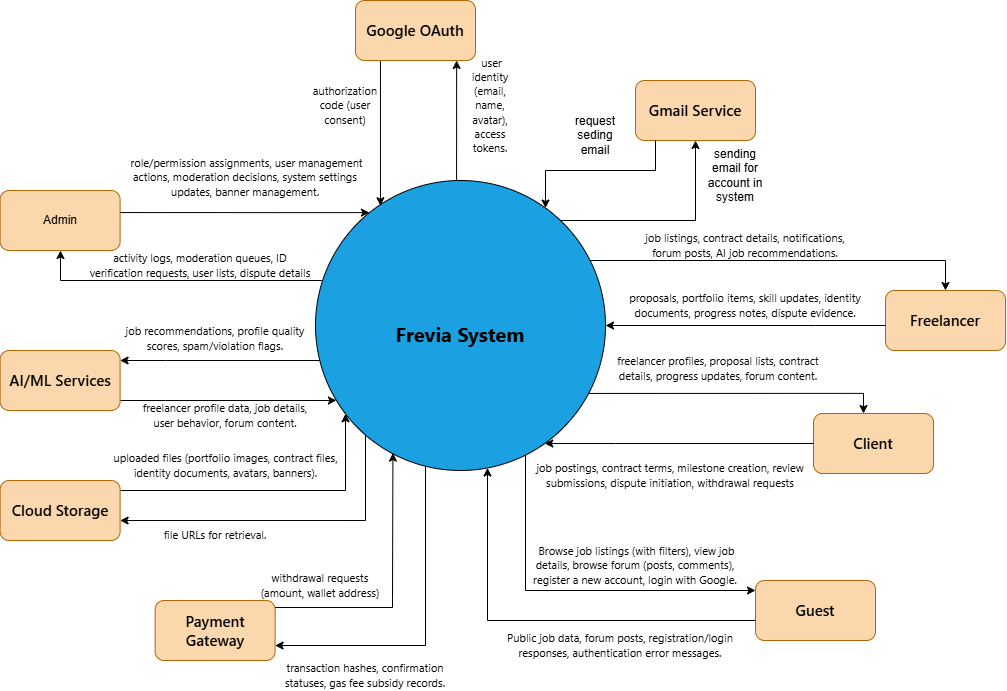
\includegraphics[width=0.9\linewidth]{image/context_diagram/context-diagram.drawio.png}
    \caption{Context diagram}
    \label{fig:context-diagram}
\end{figure}
\section{User Requirement}
\subsection{Actors}
\begin{table}[H]
\centering
\caption{Actors of the Frevia Platform}
\renewcommand{\arraystretch}{1.4}
\begin{tabular}{|c|p{2.5cm}|p{10cm}|}
\hline
\rowcolor{headerbg}
\multicolumn{1}{|c|}{\textbf{No}} &
\multicolumn{1}{c|}{\textbf{Actor}} &
\multicolumn{1}{c|}{\textbf{Description}} \\
\hline

1 & Guest &
Guests are unregistered visitors who have not yet created an account on the platform. They can browse publicly available information such as job listings, freelancer profiles, forum content, and platform features. Guests may also register a new account or authenticate using supported login methods to access platform services.
\\
\hline

2 & Client &
Clients are individuals or organizations seeking professional services from freelancers. They can create and manage job postings, review proposals, hire freelancers, establish contracts, manage escrow payments, monitor project progress, initiate disputes, and provide reviews upon project completion.
\\
\hline

3 & Freelancer &
Freelancers are service providers who offer professional skills and expertise through the platform. They can create and manage profiles, portfolios, and skills; search and apply for jobs; submit proposals; collaborate with clients; complete project tasks and milestones; and receive payments after successful project delivery.
\\
\hline

4 & Admin &
Administrators are responsible for managing and maintaining the platform's operations, security, and compliance. Their responsibilities include user management, role and permission management, identity verification, content moderation, dispute resolution, system configuration, and monitoring platform activities to ensure a secure and reliable environment.
\\
\hline

\end{tabular}
\label{tab:actors}
\end{table}

\subsection{Use Cases}
\subsubsection{Diagram(s)}
% Guest

\begin{figure}[H]
    \centering
    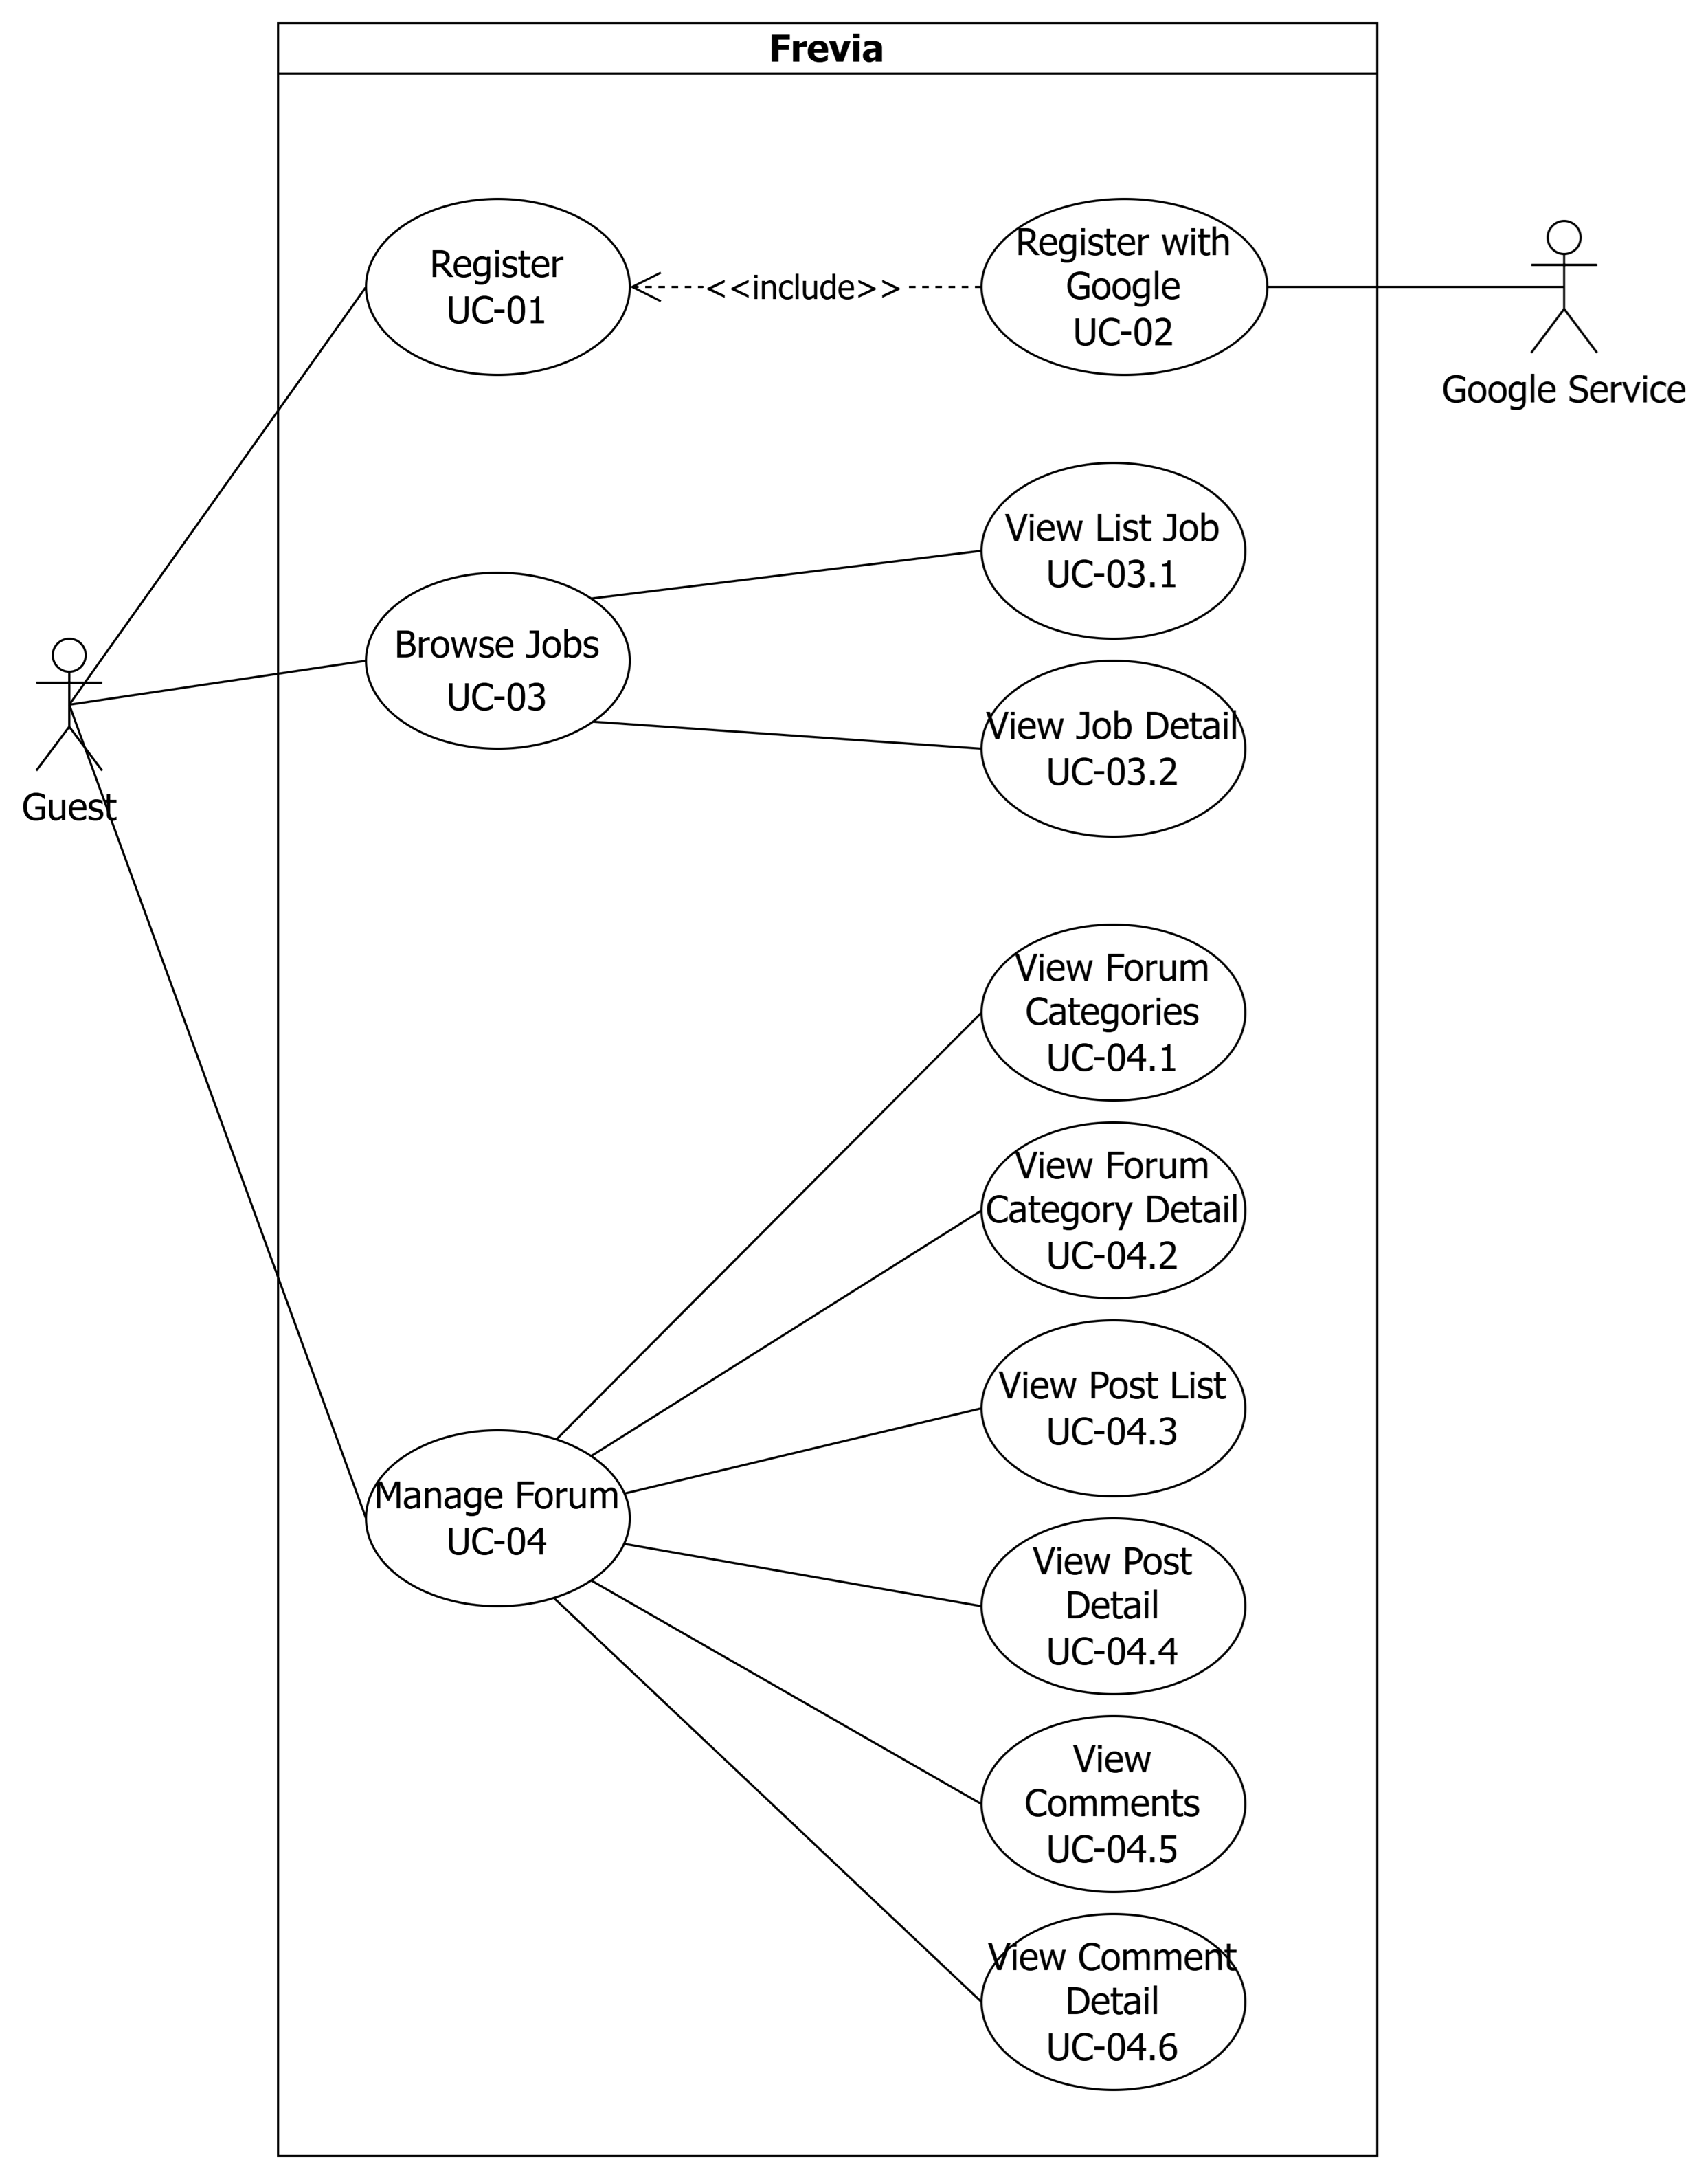
\includegraphics[width=0.95\textwidth]{image/UC_diagram/GUEST_SP1.png}
    \caption{Guest Usecase}
    \label{fig:Guest Usecase}
\end{figure}

% Client

\begin{figure}[H]
    \centering
    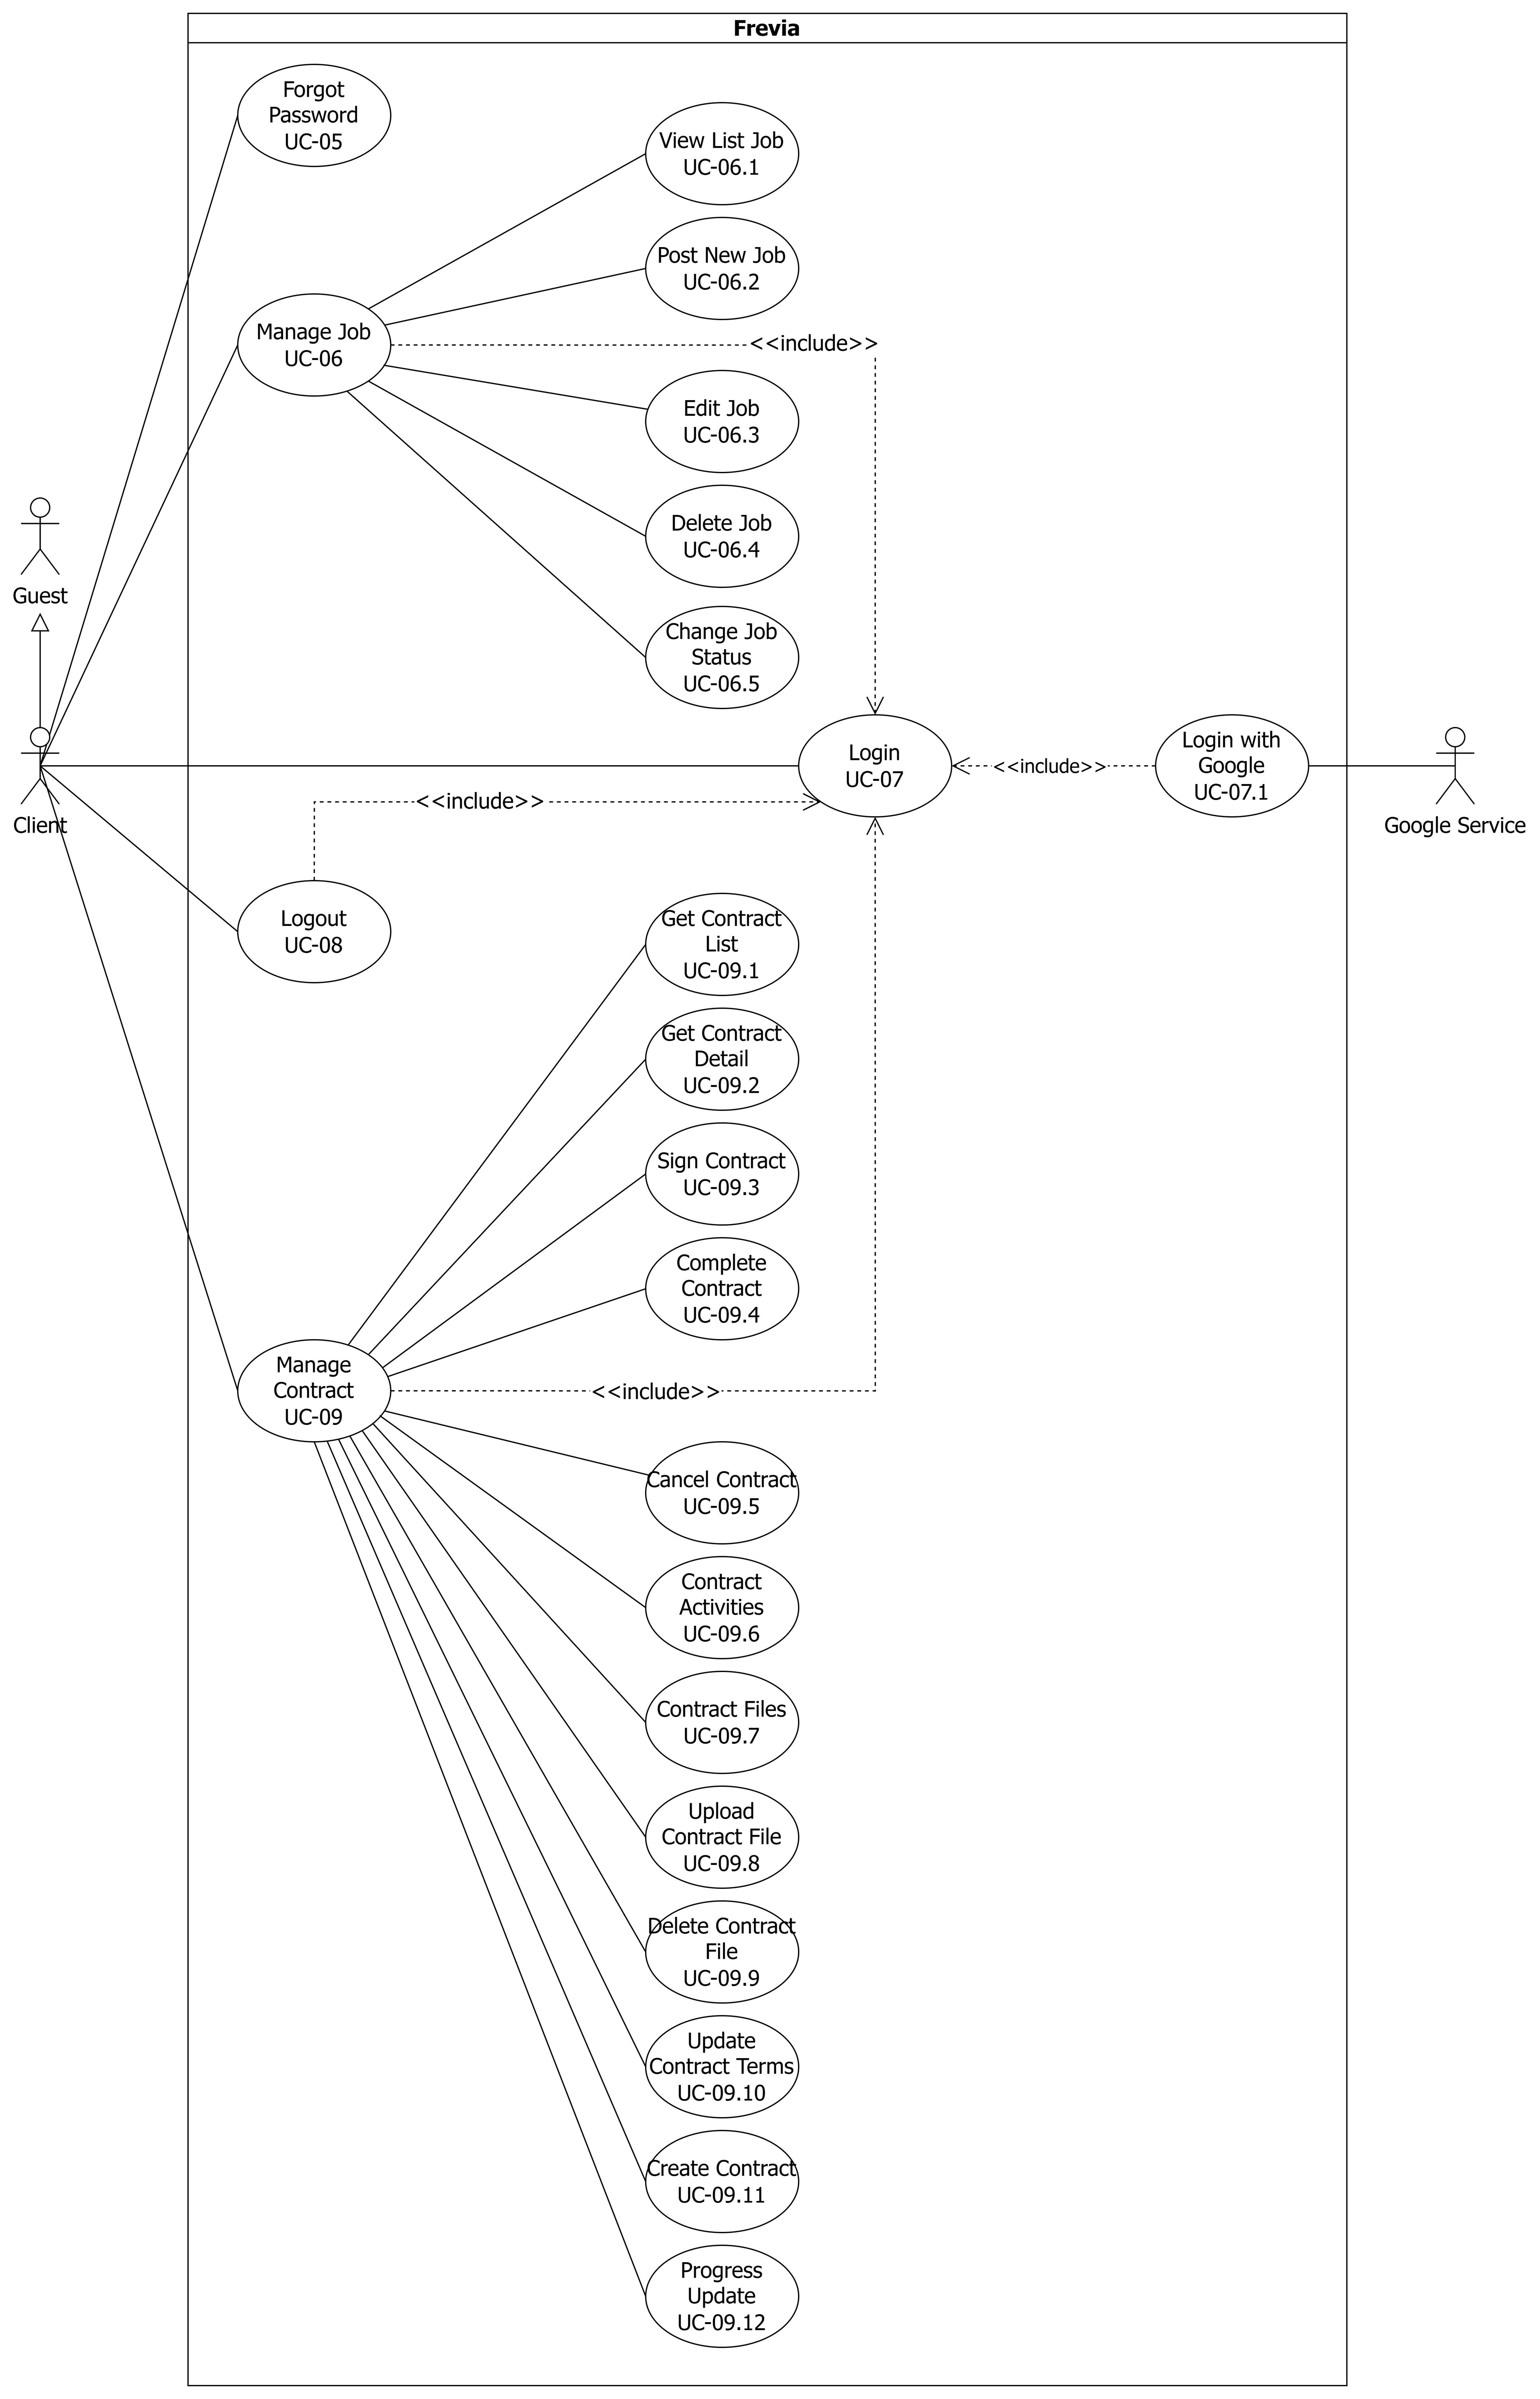
\includegraphics[
            width=\textwidth,
        height=0.85\textheight,
        keepaspectratio
    ]{image/UC_diagram/CLIENT1_SP1.png}
    \caption{Client Usecase}
    \label{fig:Client Usecase}
\end{figure}

\begin{figure}[H]
    \centering
    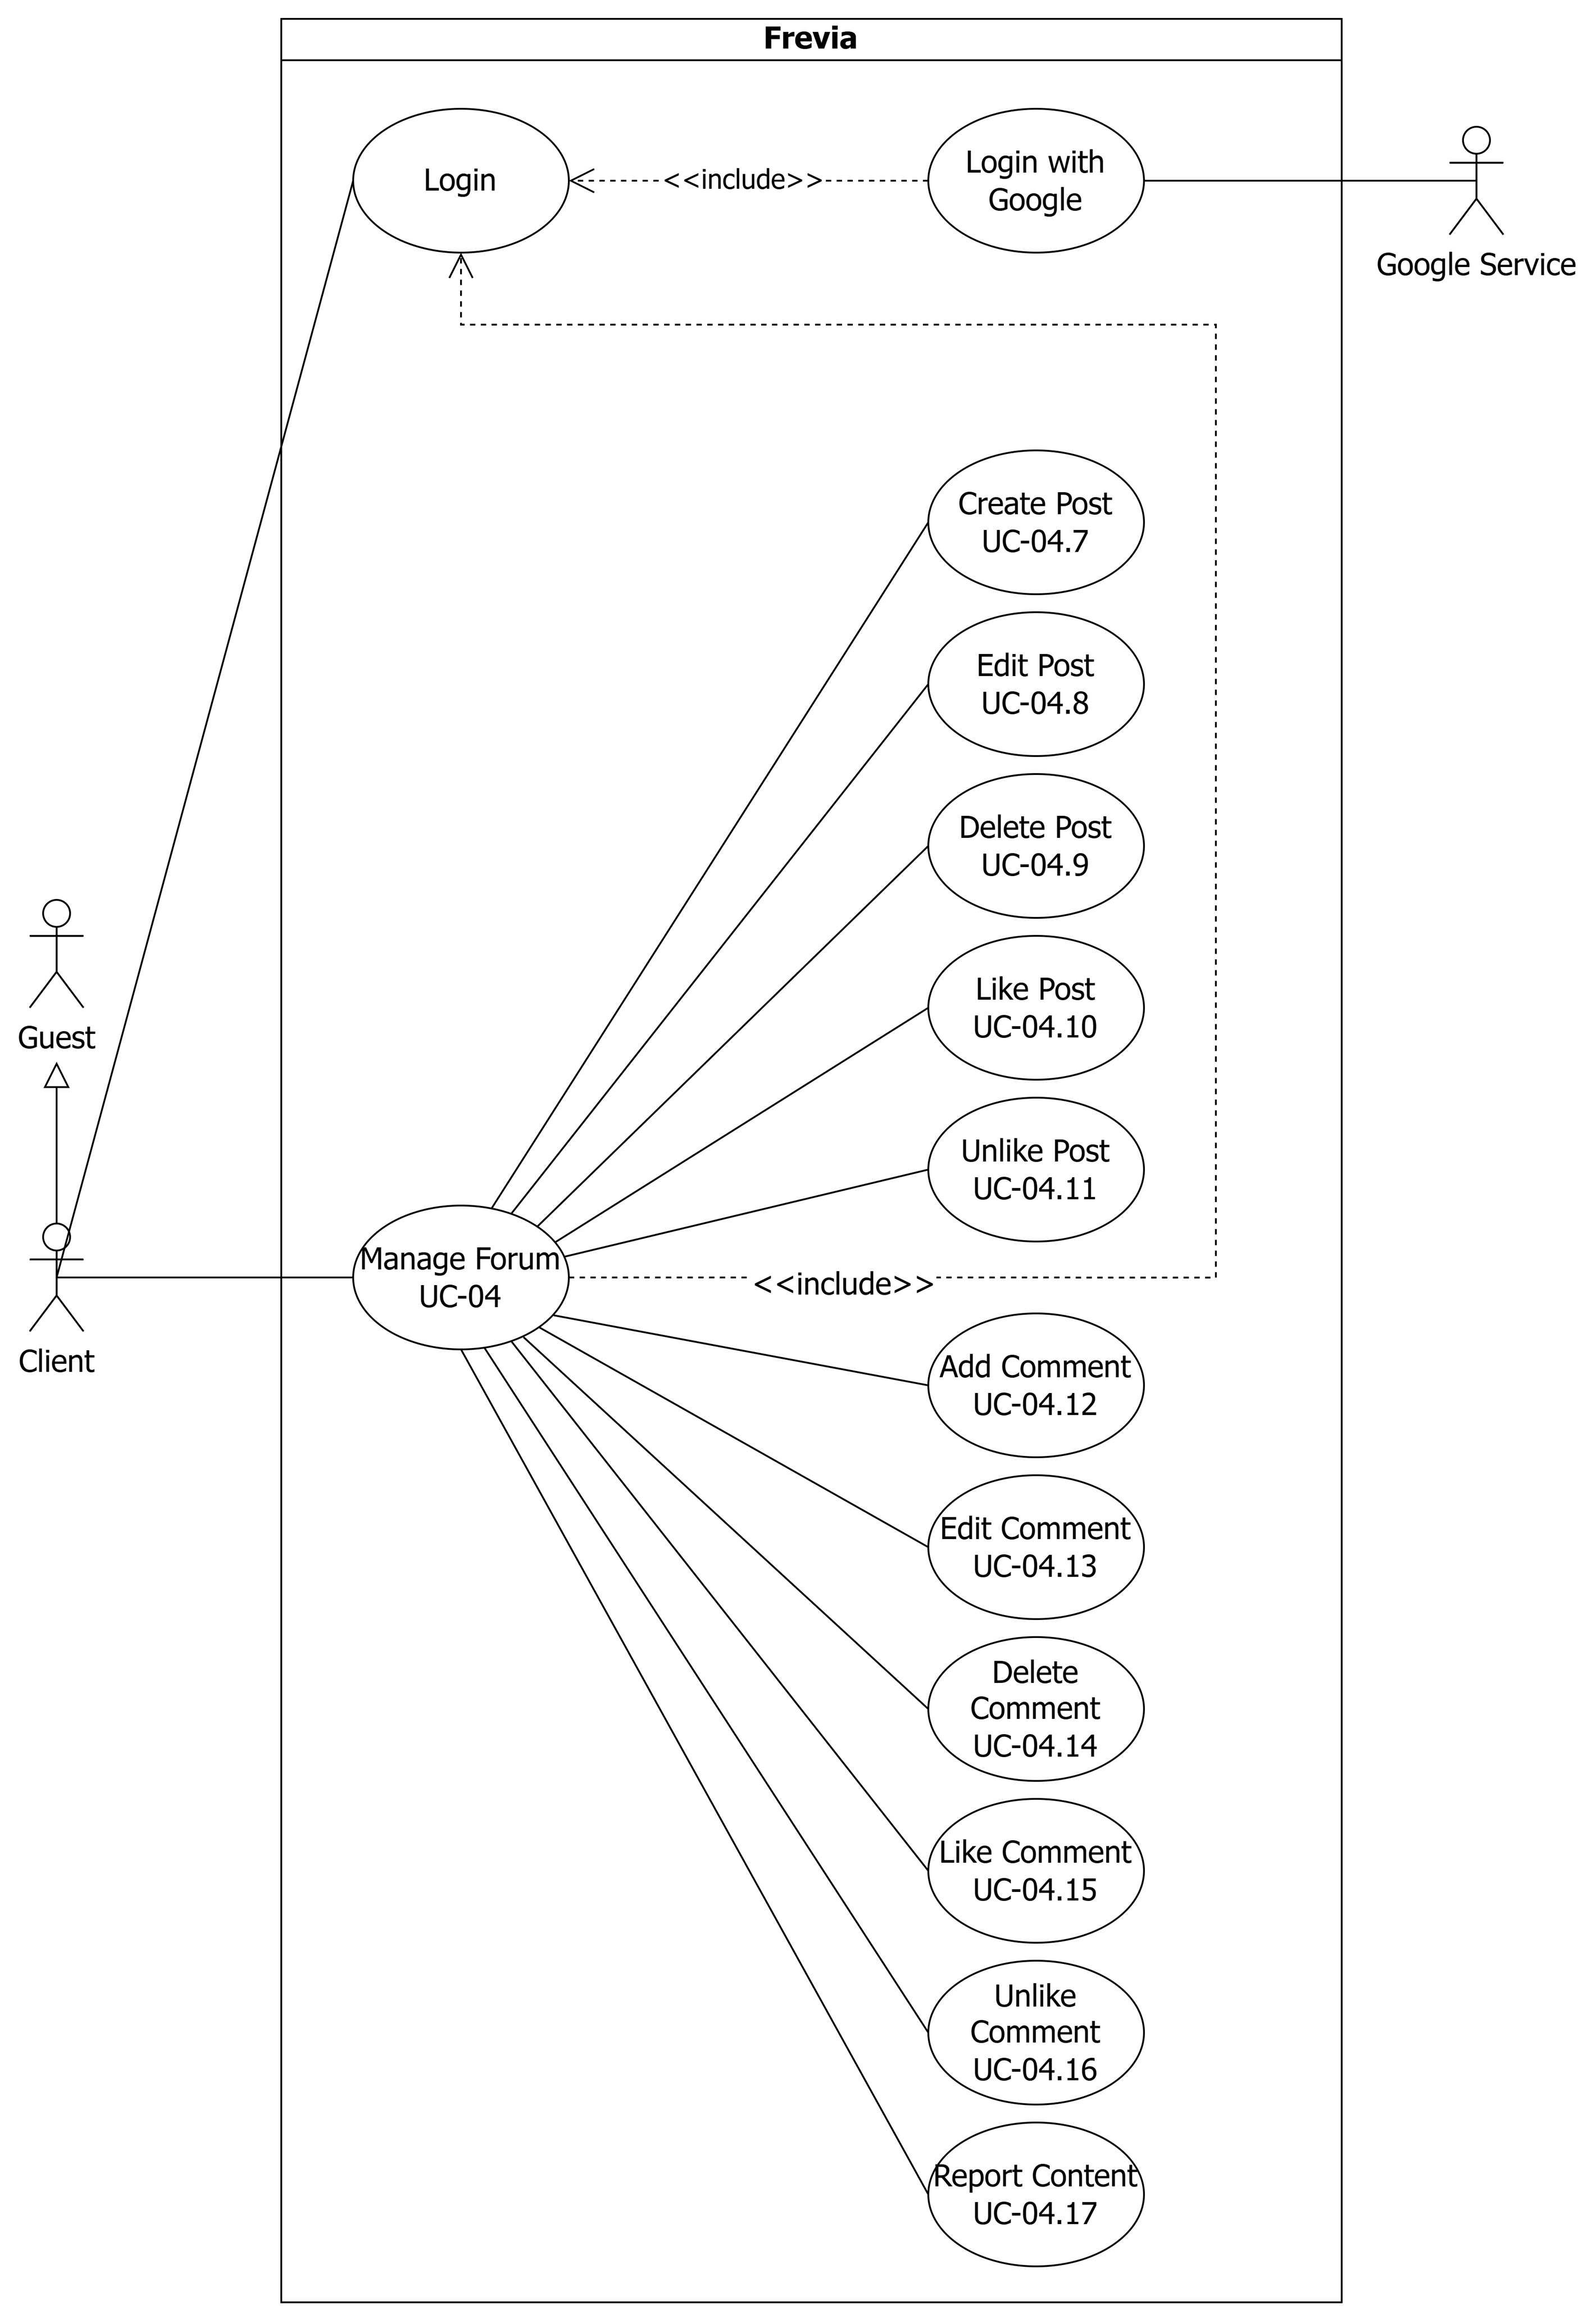
\includegraphics[
            width=\textwidth,
        height=0.85\textheight,
        keepaspectratio
    ]{image/UC_diagram/CLIENT2_SP1.png}
    \caption{Client Usecase}
    \label{fig:Client Usecase}
\end{figure}


% Freelancer
\begin{figure}[H]
    \centering
    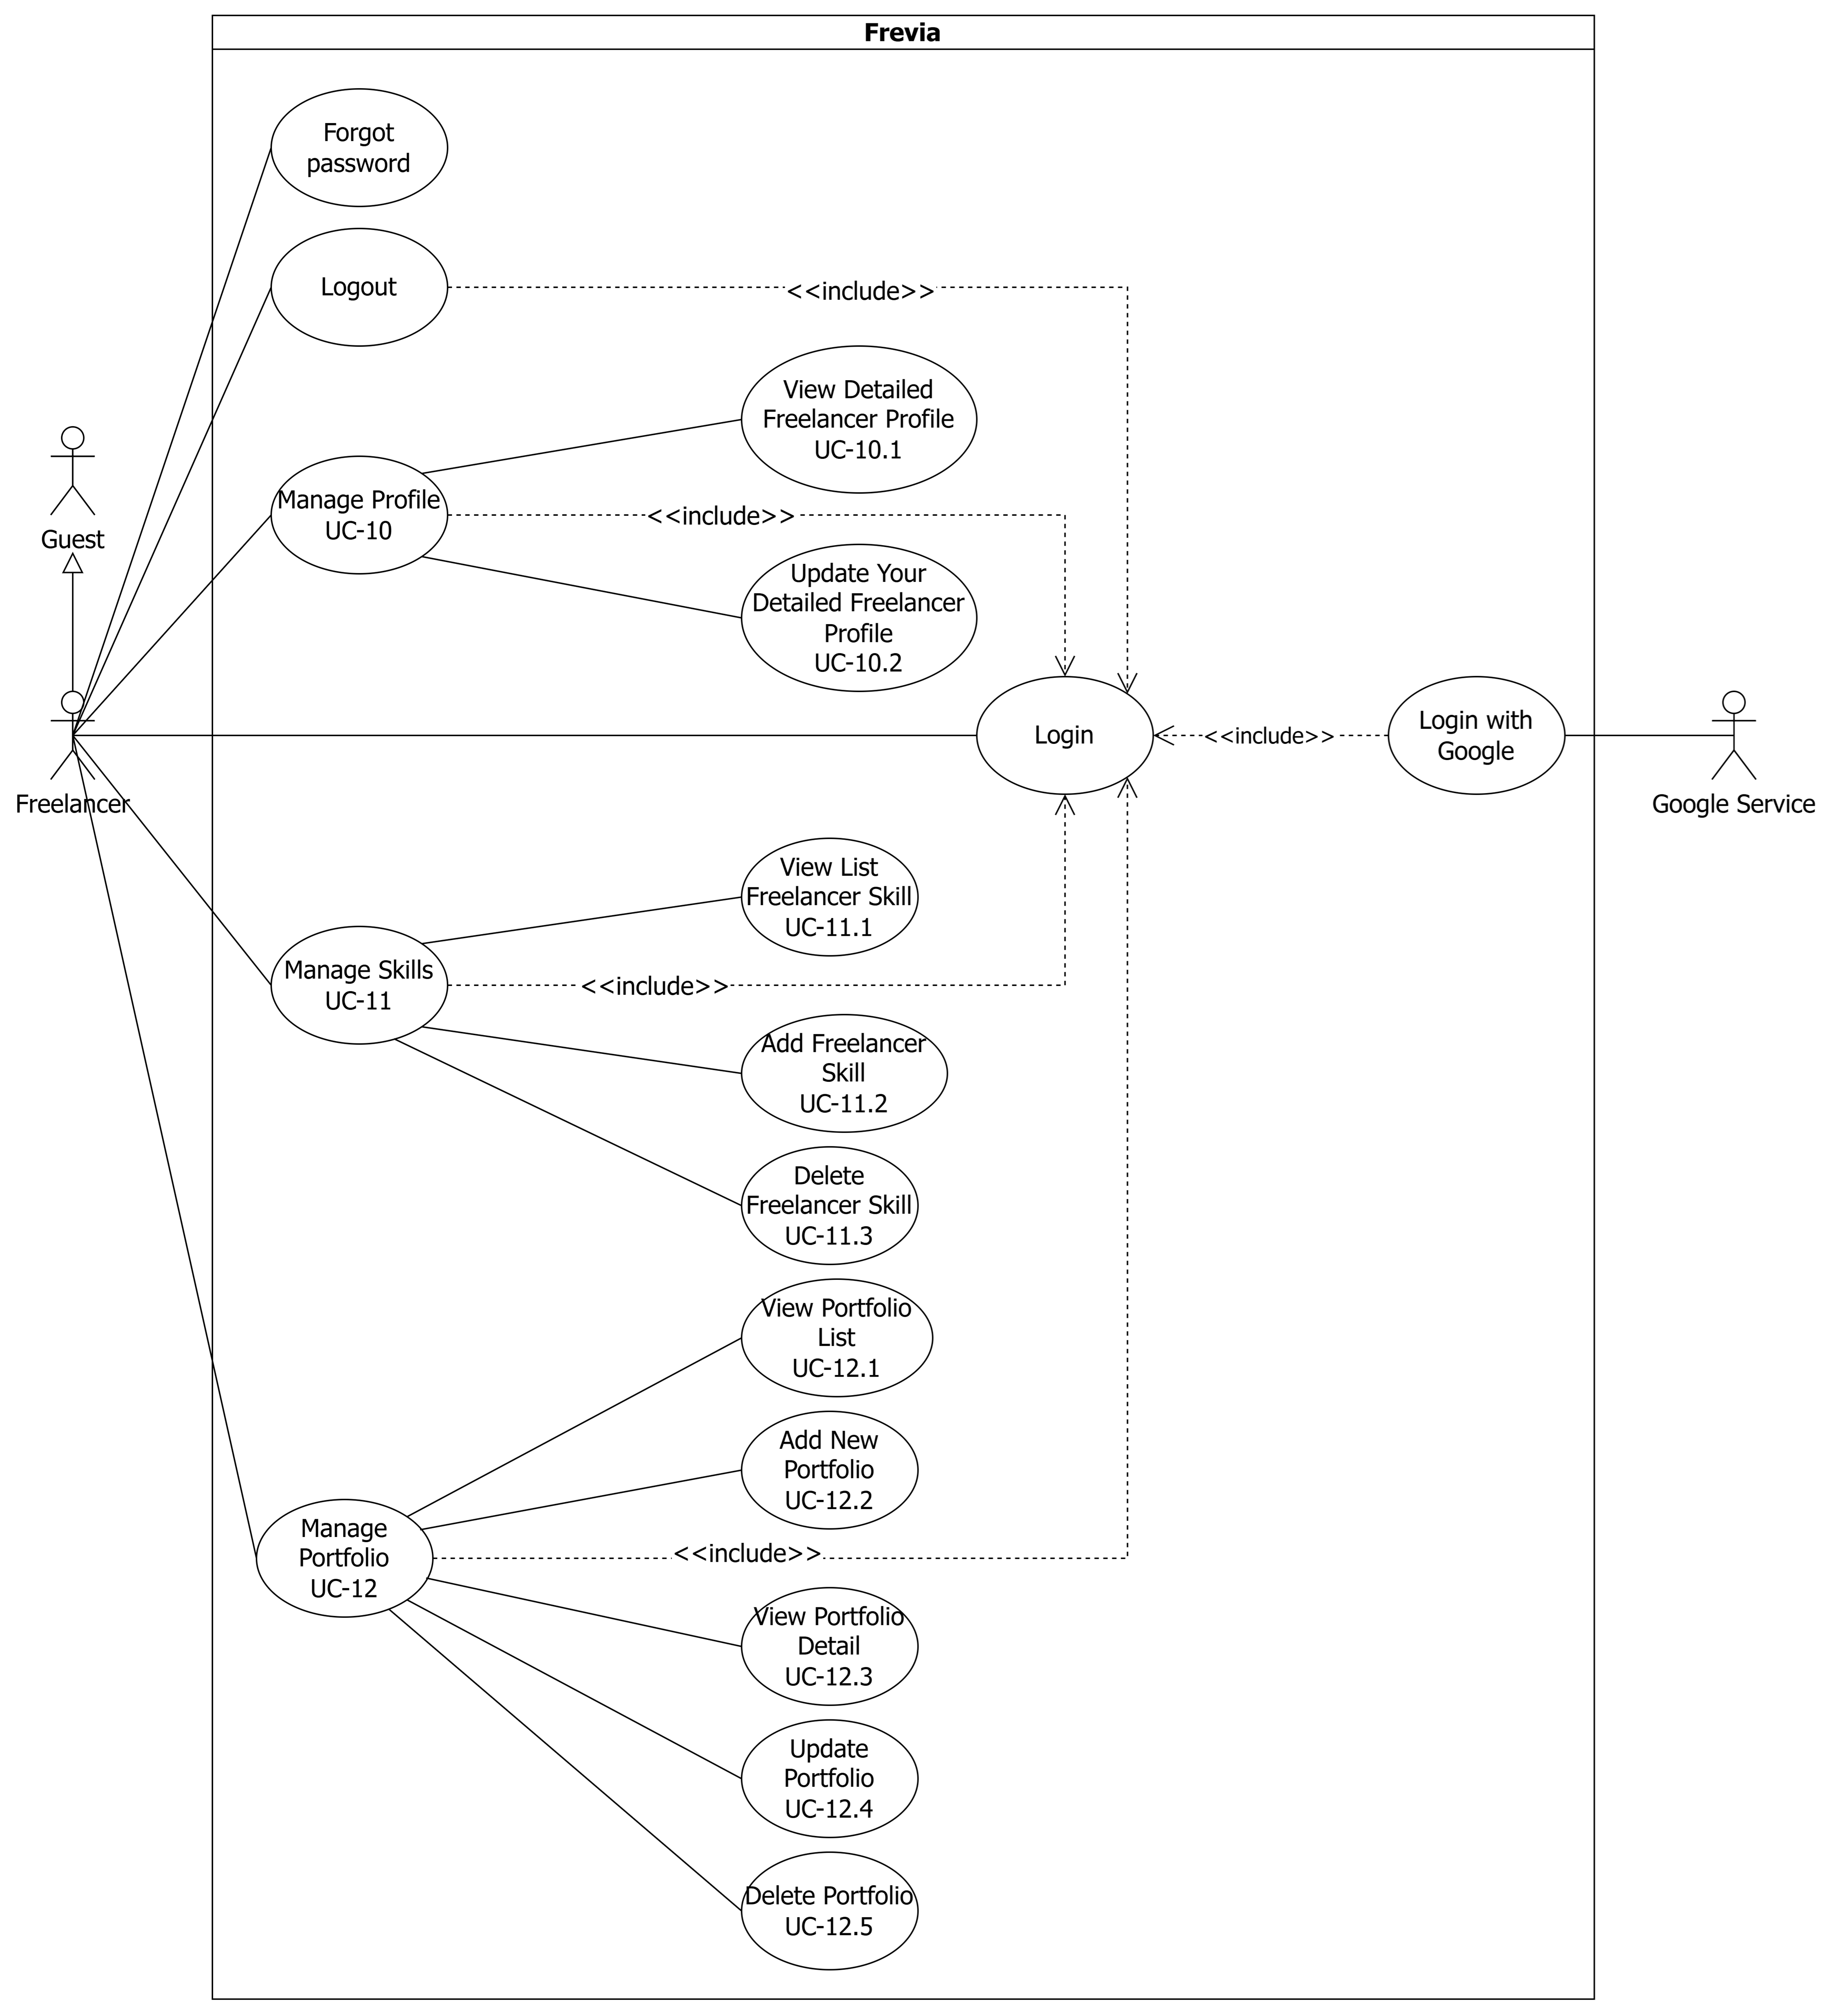
\includegraphics[
            width=\textwidth,
        height=0.85\textheight,
        keepaspectratio
    ]{image/UC_diagram/FREE1_SP1.png}
    \caption{Freelancer Usecase}
    \label{fig:Freelancer Usecase}
\end{figure}

\begin{figure}[H]
    \centering
    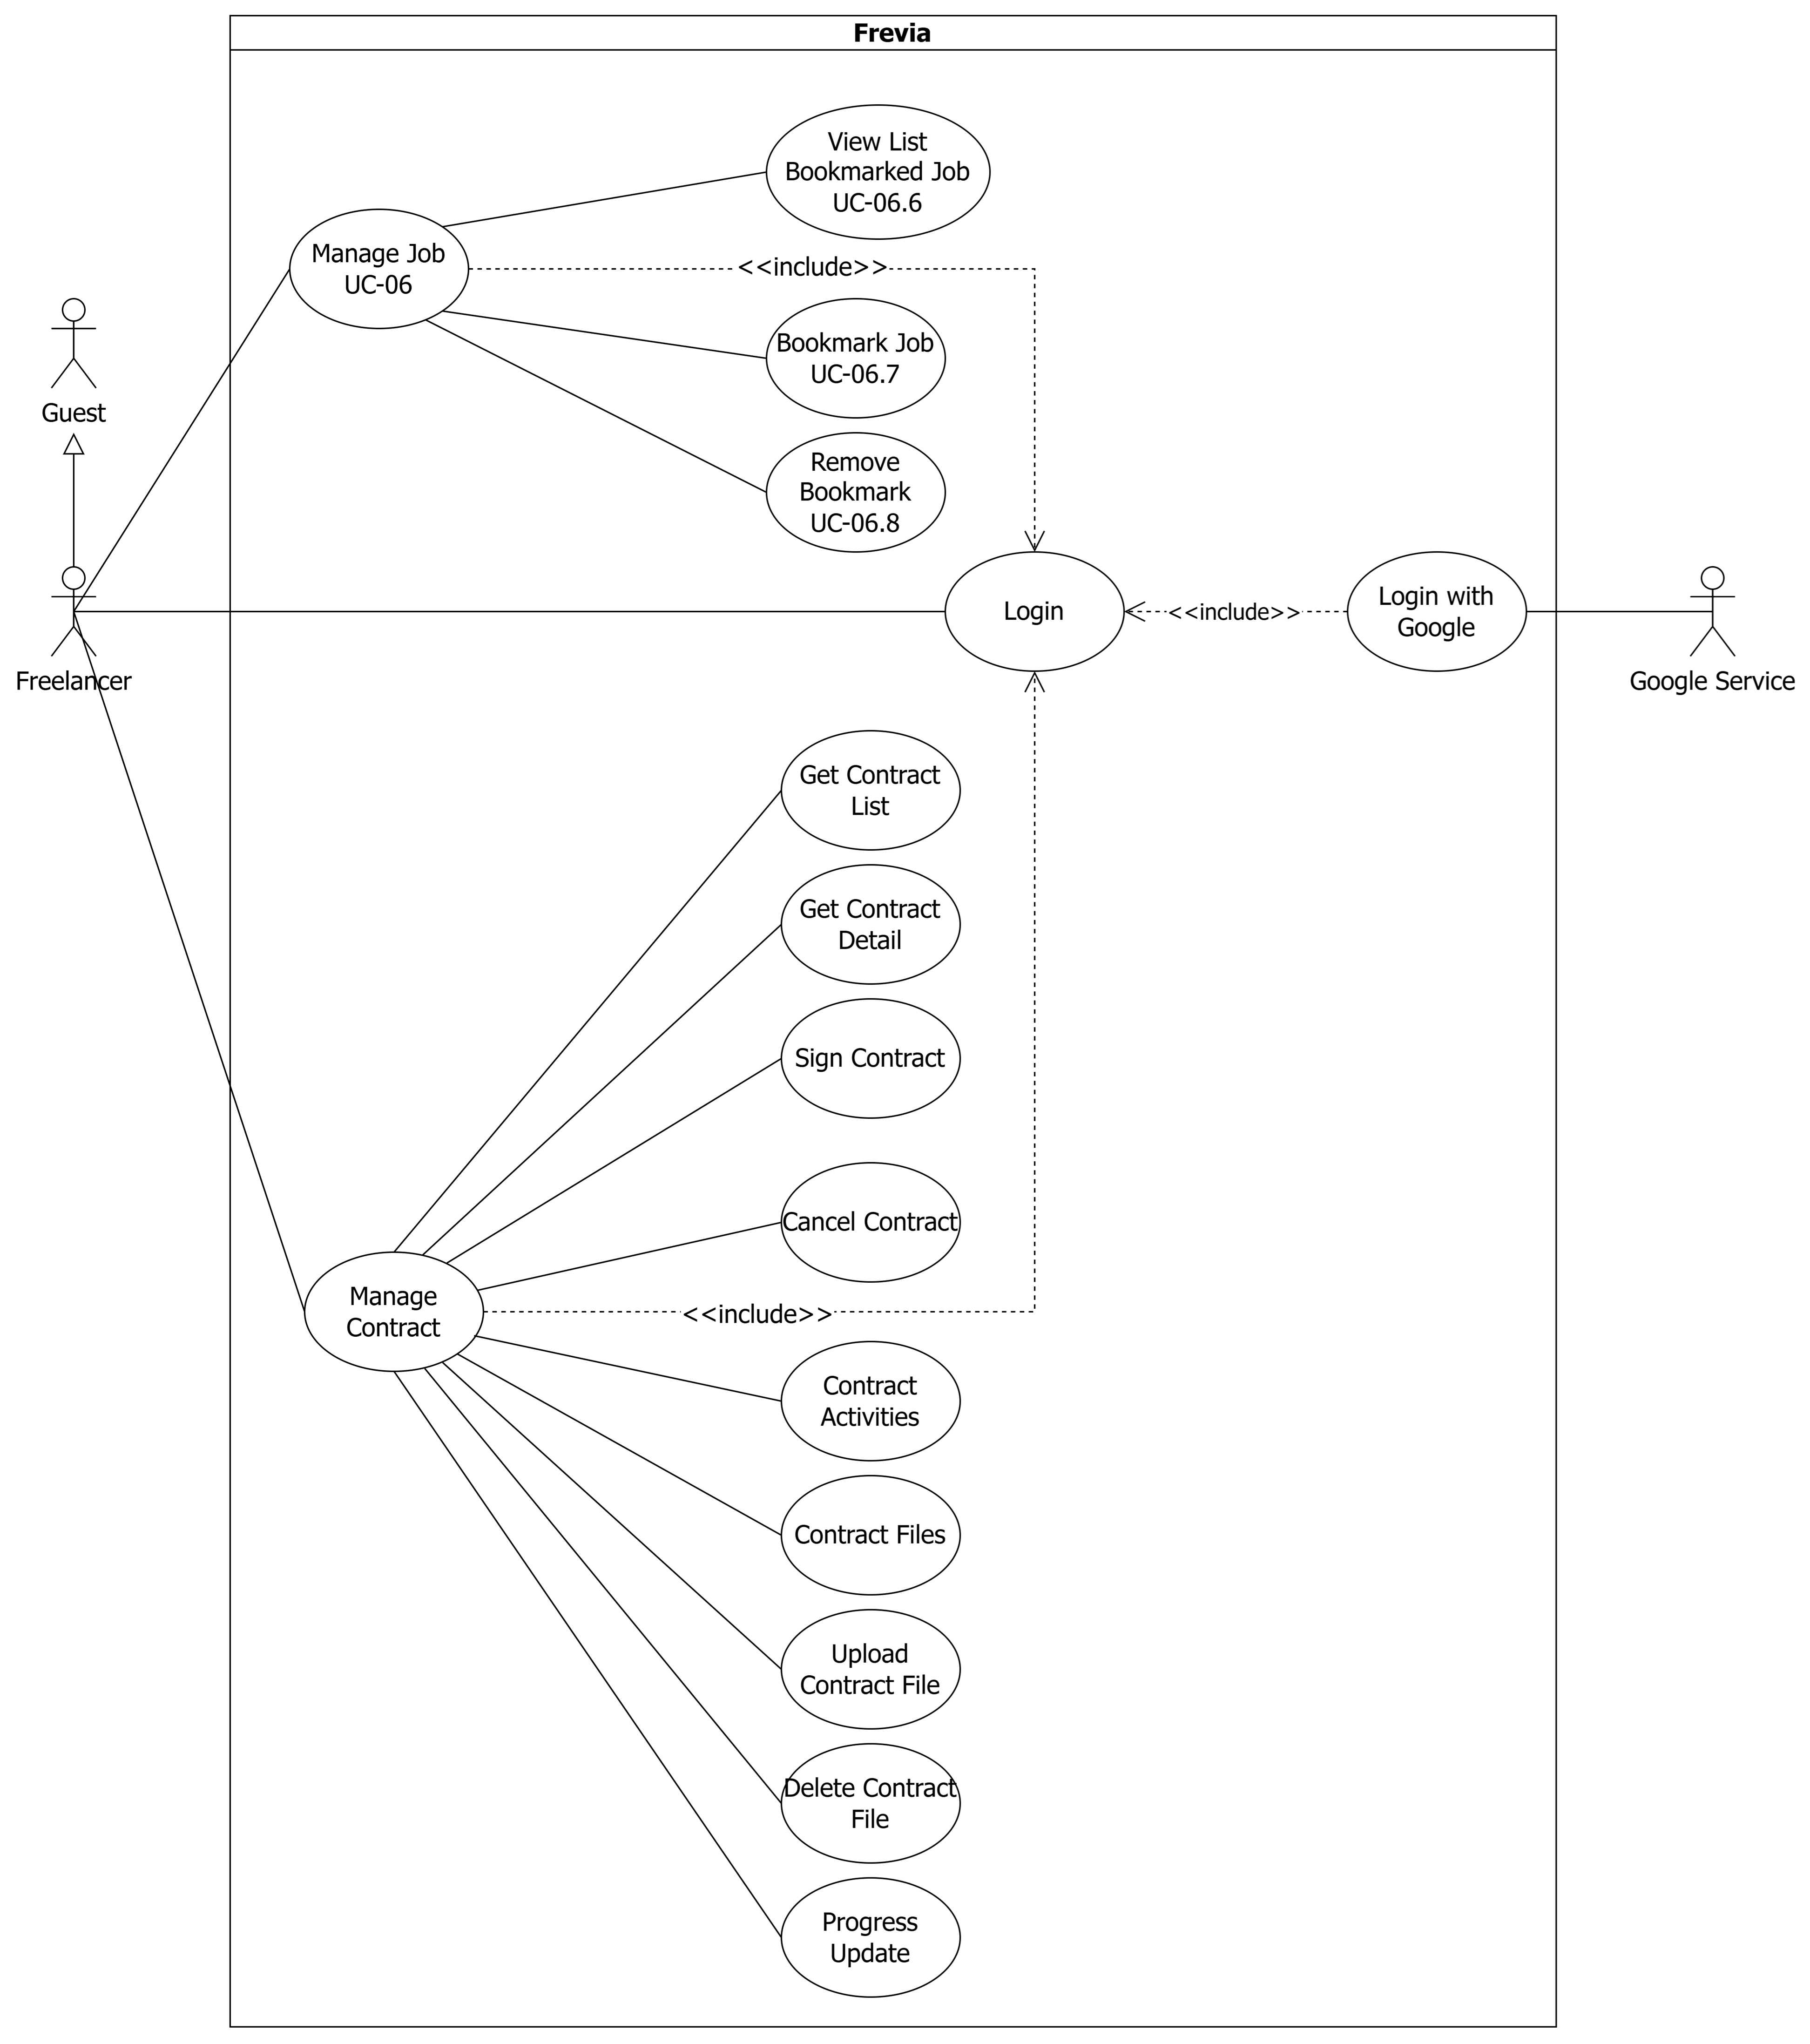
\includegraphics[
            width=\textwidth,
        height=0.85\textheight,
        keepaspectratio
    ]{image/UC_diagram/FREE2_SP1.png}
    \caption{Freelancer Usecase}
    \label{fig:Freelancer Usecase}
\end{figure}

\begin{figure}[H]
    \centering
    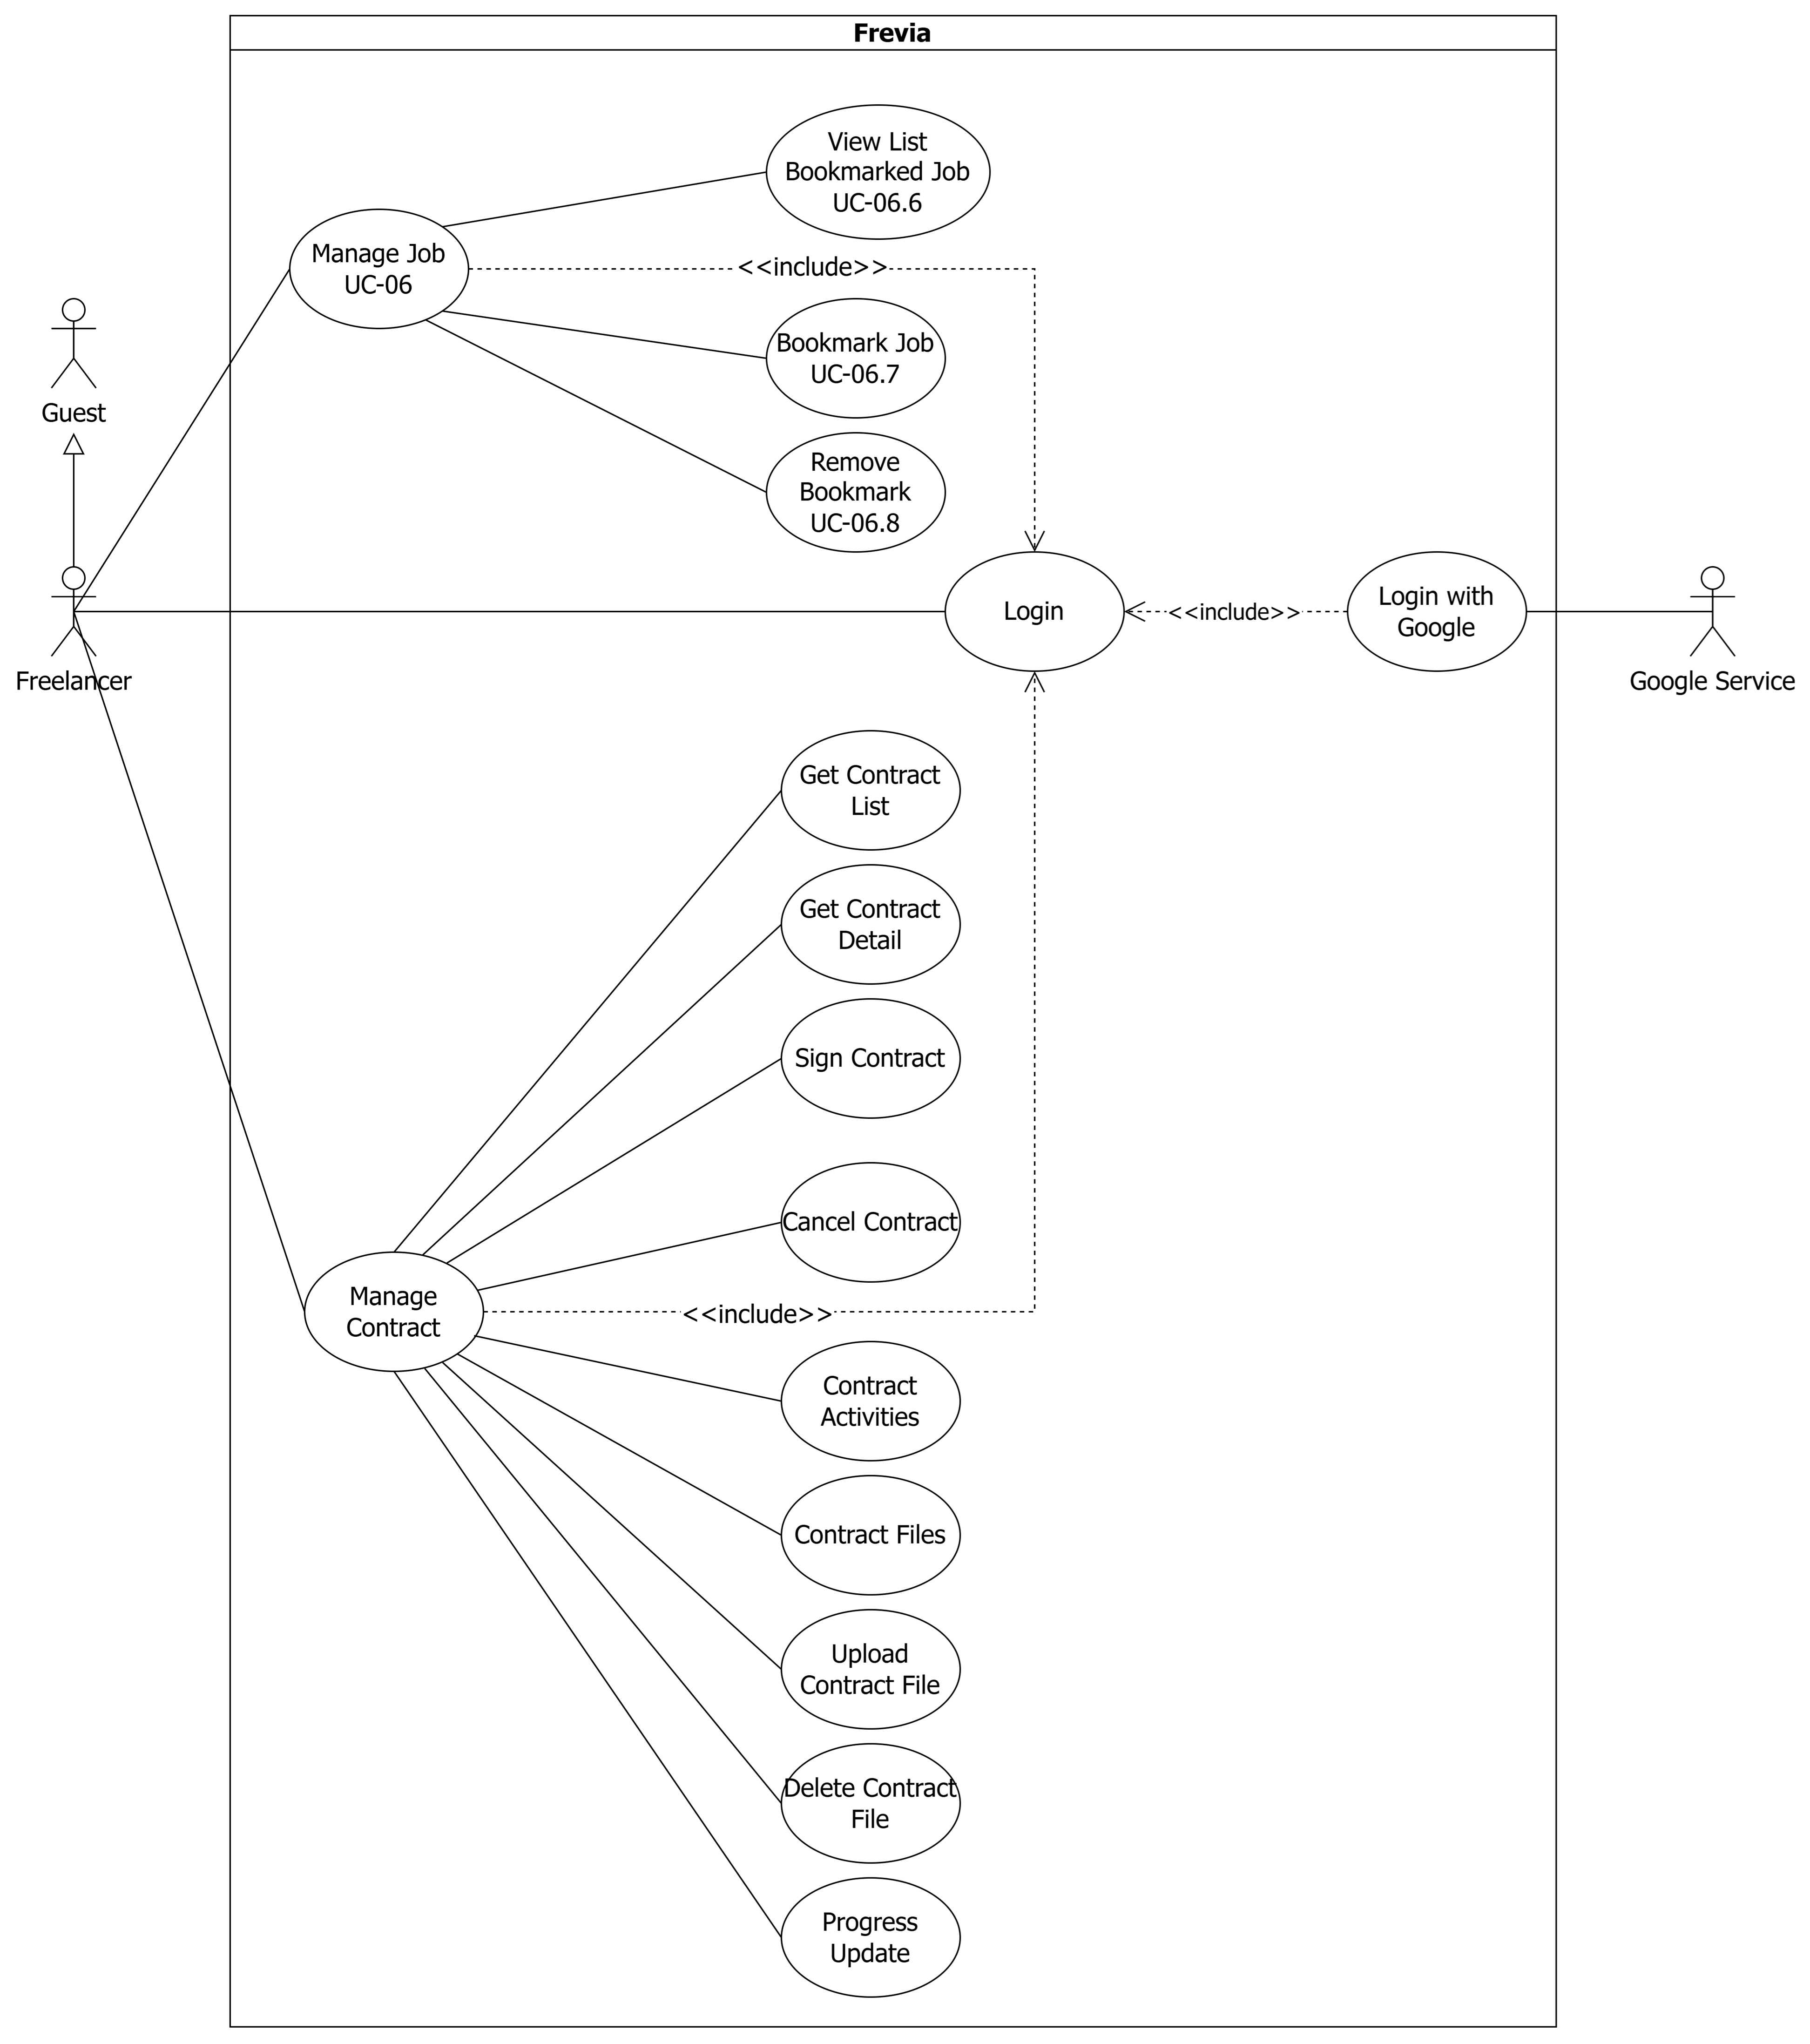
\includegraphics[
            width=\textwidth,
        height=0.85\textheight,
        keepaspectratio
    ]{image/UC_diagram/FREE2_SP1.png}
    \caption{Freelancer Usecase}
    \label{fig:Freelancer Usecase}
\end{figure}

% Admin

\begin{figure}[H]
    \centering
    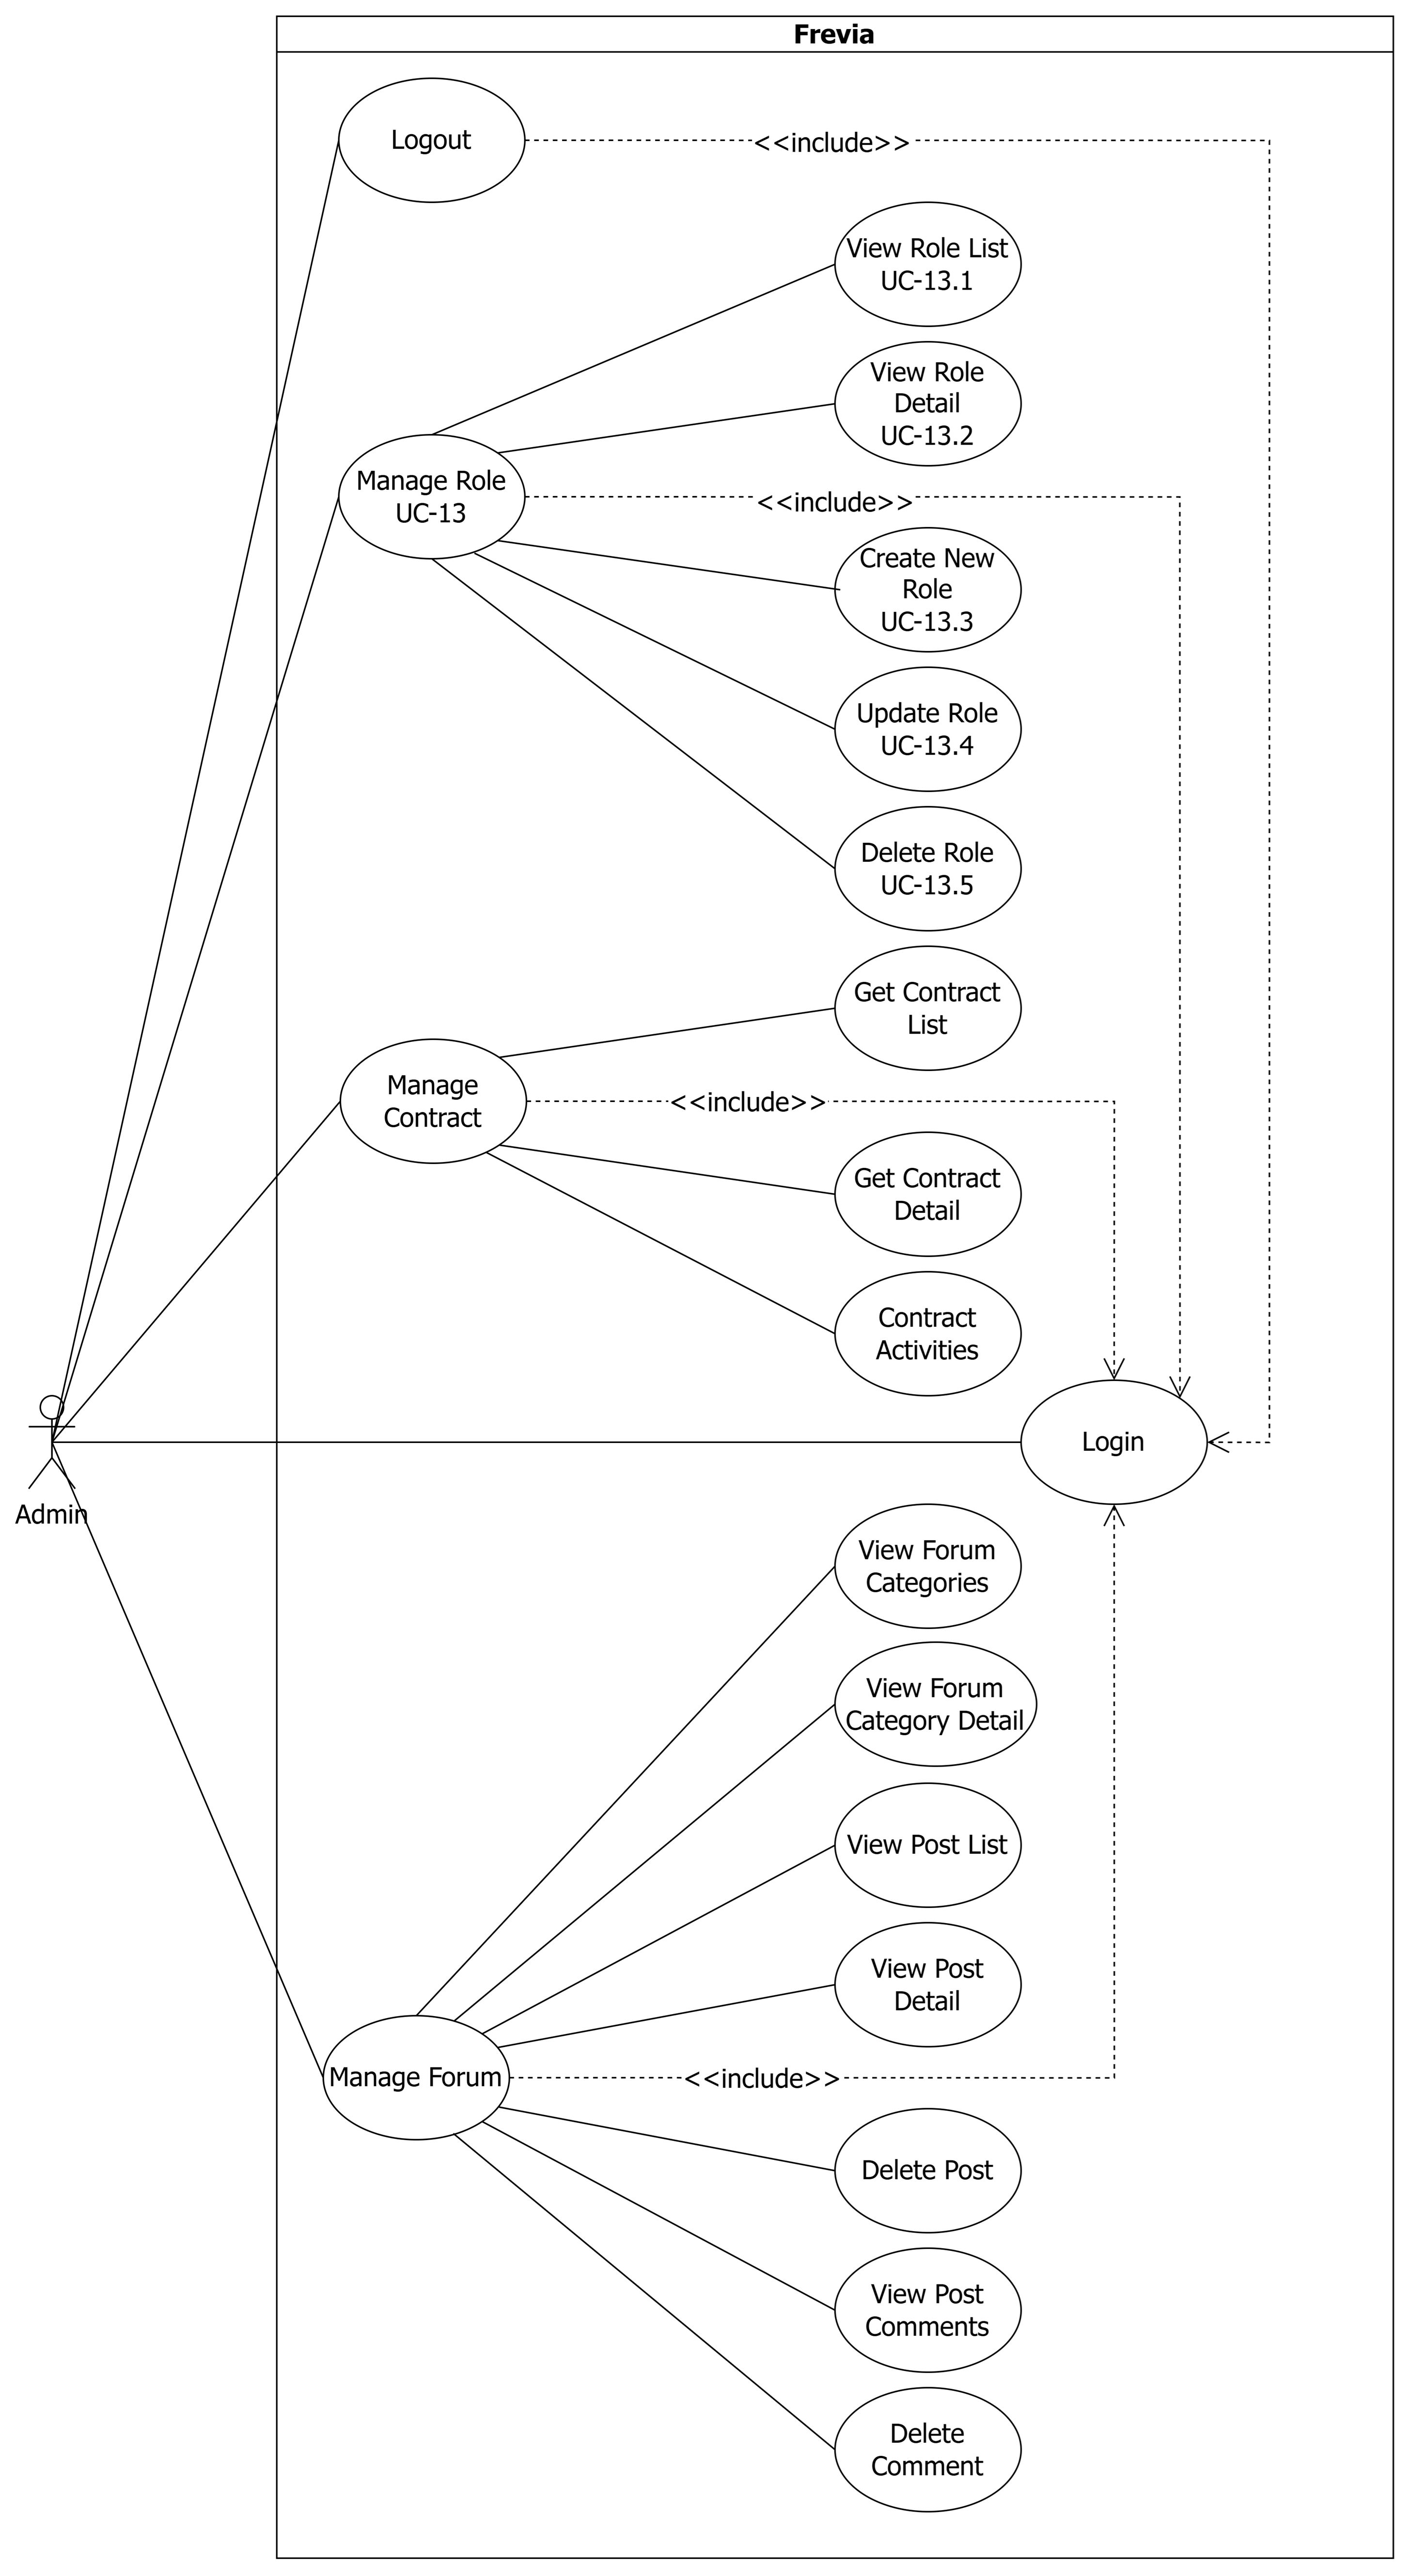
\includegraphics[
            width=\textwidth,
        height=0.85\textheight,
        keepaspectratio
    ]{image/UC_diagram/ADMIN_SP1.png}
    \caption{Admin Usecase}
    \label{fig:Admin Usecase}
\end{figure}

\subsubsection{Use Case Description}
\begin{longtable}{|>{\raggedright\arraybackslash}p{2.2cm}|>{\raggedright\arraybackslash}p{3cm}|>{\raggedright\arraybackslash}p{3cm}|>{\raggedright\arraybackslash}p{7.5cm}|}
\hline
\rowcolor{headerbg}
\multicolumn{1}{|>{\raggedright\arraybackslash}p{2.2cm}|}{\textbf{ID}} &
\multicolumn{1}{>{\raggedright\arraybackslash}p{3cm}|}{\textbf{Use Case}} &
\multicolumn{1}{>{\raggedright\arraybackslash}p{3cm}|}{\textbf{Actors}} &
\multicolumn{1}{>{\raggedright\arraybackslash}p{7.5cm}|}{\textbf{Description}} \\
\hline
\endfirsthead

\hline
\rowcolor{headerbg}
\multicolumn{1}{|>{\raggedright\arraybackslash}p{2.2cm}|}{\textbf{ID}} &
\multicolumn{1}{>{\raggedright\arraybackslash}p{3cm}|}{\textbf{Use Case}} &
\multicolumn{1}{>{\raggedright\arraybackslash}p{3cm}|}{\textbf{Actors}} &
\multicolumn{1}{>{\raggedright\arraybackslash}p{7.5cm}|}{\textbf{Description}} \\
\hline
\endhead

\hline
\multicolumn{4}{r}{\textit{Continued on next page}} \\
\endfoot

\hline
\endlastfoot


UC-01 & Register & Guest, Client, Freelancer & Allows users to create new accounts using email and password. \\
\hline
UC-02 & Google Login & Guest, Client, Freelancer & Allows users to login/register using Google OAuth. \\
\hline
UC-03 & Job Browsing & Guest, Client, Freelancer & Enables guests to browse and search for available job listings. \\
\hline
UC-03.1 & View List Job & Guest, Client, Freelancer & Retrieve paginated job list with filters (category, budget, skills, status, keywords) and sorting options. \\
\hline
UC-03.2 & View Job Detail & Guest, Client, Freelancer & Get full job details: title, description, budget, skills, client info, proposals count, attachments, timeline. \\
\hline
UC-04 & Manage Forum & Guest, Client, Freelancer, Admin & Manages forum operations including viewing, creating, editing, and moderating posts and comments. \\
\hline
UC-04.1 & View Forum Categories & Guest, Client, Freelancer, Admin & Displays all available forum categories for browsing. \\
\hline
UC-04.2 & View Forum Category Detail & Guest, Client, Freelancer, Admin & Shows detailed information of a specific forum category and its sub-forums. \\
\hline
UC-04.3 & View Post List & Guest, Client, Freelancer, Admin & Retrieves paginated list of posts within a forum category with filters and sorting. \\
\hline
UC-04.4 & View Post Detail & Guest, Client, Freelancer, Admin & Displays full post content, author info, creation date, and associated tags. \\
\hline
UC-04.5 & View Comments & Guest, Client, Freelancer, Admin & Retrieves all comments related to a specific forum post. \\
\hline
UC-04.6 & View Comment Detail & Guest, Client, Freelancer, Admin & Shows detailed information of a specific comment, including content, author, and timestamps. \\
\hline
UC-04.7 & Create Post & Client, Freelancer & Allows freelancers to create new discussion posts or questions in the forum. \\
\hline
UC-04.8 & Edit Post & Client, Freelancer & Allows freelancers to edit their own forum posts. \\
\hline
UC-04.9 & Delete Post & Client, Freelancer, Admin & Allows post owners or admins to delete a forum post. \\
\hline
UC-04.10 & Like Post & Client, Freelancer & Allows freelancers to like a forum post. \\
\hline
UC-04.11 & Unlike Post & Client, Freelancer & Allows freelancers to remove their like from a forum post. \\
\hline
UC-04.12 & Add Comment & Client, Freelancer & Allows freelancers to add comments to a forum post. \\
\hline
UC-04.13 & Edit Comment & Client, Freelancer & Allows freelancers to edit their own comments. \\
\hline
UC-04.14 & Delete Comment & Client, Freelancer & Allows comment owners or admins to delete a comment. \\
\hline
UC-04.15 & Like Comment & Client, Freelancer & Allows freelancers to like a comment. \\
\hline
UC-04.16 & Unlike Comment & Client, Freelancer & Allows freelancers to remove their like from a comment. \\
\hline
UC-04.17 & Report Content & Client, Freelancer & Allows freelancers to report inappropriate content in forum posts or comments. \\
\hline
UC-05 & Forgot Password & Client, Freelancer & Allows users to reset their password via email verification. \\
\hline
UC-06 & Manage Job & Client, Freelancer & Manages job postings including creation, editing, deletion, and status changes. \\
\hline
UC-06.1 & View List Job & Guest, Client, Freelancer & Retrieve paginated job list with filters and sorting options. \\
\hline
UC-06.2 & Post New Job & Client & Allows clients to create and publish new job postings. \\
\hline
UC-06.3 & Edit Job & Client & Allows clients to edit their own job postings. \\
\hline
UC-06.4 & Delete Job & Client & Allows clients to delete their own job postings. \\
\hline
UC-06.5 & Change Job Status & Client & Allows clients to update job status (Open, In Progress, Closed, Cancelled). \\
\hline
UC-06.6 & View List Bookmarked Job & Freelancer & Retrieves list of jobs bookmarked by the freelancer. \\
\hline
UC-06.7 & Bookmark Job & Freelancer & Allows freelancers to save/bookmark a job for later reference. \\
\hline
UC-06.8 & Remove Bookmark & Freelancer & Allows freelancers to remove a bookmarked job from their list. \\
\hline
UC-07 & Login & Client, Freelancer, Admin & Allows users to authenticate using email and password. \\
\hline
UC-08 & Logout & Client, Freelancer, Admin & Allows users to securely log out of the system. \\
\hline
UC-09 & Manage Contract & Client, Freelancer, Admin & Manages contracts between clients and freelancers. \\
\hline
UC-09.1 & Get Contract List & Client, Freelancer, Admin & Retrieves paginated list of contracts with status filters and sorting. \\
\hline
UC-09.2 & Get Contract Detail & Client, Freelancer, Admin & Displays full contract details including terms, parties, status, and milestones. \\
\hline
UC-09.3 & Sign Contract & Client, Freelancer & Allows freelancers to digitally sign and accept a contract. \\
\hline
UC-09.4 & Complete Contract & Client, Freelancer & Marks a contract as completed successfully. \\
\hline
UC-09.5 & Cancel Contract & Client, Freelancer & Allows either party to cancel a contract before completion. \\
\hline
UC-09.6 & Contract Activities & Client, Freelancer, Admin & Tracks all activities and updates related to a contract. \\
\hline
UC-09.7 & Contract Files & Client, Freelancer & Manages files and attachments associated with a contract. \\
\hline
UC-09.8 & Upload Contract File & Client, Freelancer & Allows users to upload files to a contract (e.g., deliverables, documents). \\
\hline
UC-09.9 & Delete Contract File & Client, Freelancer & Allows users to delete files from a contract. \\
\hline
UC-09.10 & Update Contract Terms & Client & Allows clients to update contract terms and conditions. \\
\hline
UC-09.11 & Create Contract & Client & Allows clients to create and initiate a new contract with a freelancer. \\
\hline
UC-09.12 & Progress Update & Client, Freelancer & Allows freelancers to submit progress updates on contract milestones. \\
\hline
UC-10 & Manage Profile & Freelancer & Manages freelancer profile information and settings. \\
\hline
UC-10.1 & View Detailed Freelancer Profile & Freelancer & Displays full freelancer profile including skills, portfolio, experience, and ratings. \\
\hline
UC-10.2 & Update Your Detailed Freelancer Profile & Freelancer & Allows freelancers to edit and update their profile information. \\
\hline
UC-11 & Manage Skills & Freelancer & Manages freelancer skill set and proficiency levels. \\
\hline
UC-11.1 & View List Freelancer Skill & Freelancer & Retrieve the list of skills added by the freelancer. \\
\hline
UC-11.2 & Add Freelancer Skill & Freelancer & Allows freelancers to add new skills to their profile. \\
\hline
UC-11.3 & Delete Freelancer Skill & Freelancer & Allows freelancers to remove skills from their profile. \\
\hline
UC-12 & Manage Portfolio & Freelancer & Manages freelancer portfolio projects and work samples. \\
\hline
UC-12.1 & View Portfolio List & Freelancer & Retrieve the list of portfolios created by the freelancer. \\
\hline
UC-12.2 & Add New Portfolio & Freelancer & Allows freelancers to add new portfolio items with images and descriptions. \\
\hline
UC-12.3 & View Portfolio Detail & Freelancer & Displays full details of a portfolio item including media, description, and technologies used. \\
\hline
UC-12.4 & Update Portfolio & Freelancer & Allows freelancers to edit and update their portfolio items. \\
\hline
UC-12.5 & Delete Portfolio & Freelancer & Allows freelancers to remove portfolio items. \\
\hline
UC-13 & Manage Role & Admin & Manages user roles and permissions within the system. \\
\hline
UC-13.1 & View Role List & Admin & Retrieves list of all roles in the system. \\
\hline
UC-13.2 & View Role Detail & Admin & Displays detailed information of a specific role and its permissions. \\
\hline
UC-13.3 & Create New Role & Admin & Allows admins to create new roles with custom permissions. \\
\hline
UC-13.4 & Update Role & Admin & Allows admins to edit role permissions and details. \\
\hline
UC-13.5 & Delete Role & Admin & Allows admins to delete roles from the system. \\
\hline



\end{longtable}
\label{tab:use_cases}

\subsubsection{Use Case Specification}
% ===================
% Sprint1
% ===================
\input{sections/2.Subsections/2.2.Subsections/2.2.3.Subsections/sprint1/2.2.3.1.Authentication}

\input{sections/2.Subsections/2.2.Subsections/2.2.3.Subsections/sprint1/2.2.3.2.Role_Management}

\input{sections/2.Subsections/2.2.Subsections/2.2.3.Subsections/sprint1/2.2.3.3.Profile_Management}

\input{sections/2.Subsections/2.2.Subsections/2.2.3.Subsections/sprint1/2.2.3.4.Skills_Management}

\input{sections/2.Subsections/2.2.Subsections/2.2.3.Subsections/sprint1/2.2.3.5.Portfolio_Management}

\input{sections/2.Subsections/2.2.Subsections/2.2.3.Subsections/sprint1/2.2.3.6.Job_Browsing}

\input{sections/2.Subsections/2.2.Subsections/2.2.3.Subsections/sprint1/2.2.3.7.Job_Management}

\input{sections/2.Subsections/2.2.Subsections/2.2.3.Subsections/sprint1/2.2.3.8.Contract_Management}

\input{sections/2.Subsections/2.2.Subsections/2.2.3.Subsections/sprint1/2.2.3.9.Forum_Management}

% ===================
% Sprint2
% ===================
\section{Business Rule}

\renewcommand{\arraystretch}{1.5}

% Đổi p{2.2cm} thành 'c' để cột tự động khít với nội dung dài nhất
\begin{longtable}{|c|p{12cm}|}

\caption{Business Rules}
\label{tab:businessrules}
\\

\hline
\rowcolor{orange!30} 
\textbf{ID} 
&
\centering\arraybackslash\textbf{Rule Definition}
\\ \hline
\endfirsthead

\hline
\rowcolor{orange!30}
\textbf{ID}
&
\centering\arraybackslash\textbf{Rule Definition}
\\ \hline
\endhead

\hline
\endfoot

\hline
\endlastfoot

    BR-PROF-01 & Both basic details (from profiles) and professional details (from freelancer\_profiles) must be presented together. \\ \hline
    BR-PROF-02 & Hidden or private fields should not be displayed to unauthorized users (e.g., clients vs. the profile owner). \\ \hline
    BR-PROF-03 & Freelancers can only update their own profile. \\ \hline
    BR-PROF-04 & Mandatory fields (e.g., display\_name, title) cannot be left empty. \\ \hline
    BR-SKILL-01 & All skills belonging to the freelancer must be displayed along with their proficiency level. \\ \hline
    BR-SKILL-02 & A freelancer cannot add duplicate skills. \\ \hline
    BR-SKILL-03 & Both skill name and proficiency level are required. \\ \hline
    BR-SKILL-04 & Skill deletion must be a hard delete operation; the record is permanently removed from the mapping table. \\ \hline
    BR-SKILL-05 & Only the owning freelancer or an administrator can delete a skill from the profile. \\ \hline
    BR-PORT-01 & Only portfolios with deleted\_at = NULL shall be displayed. \\ \hline
    BR-PORT-02 & Portfolio title is a required field. \\ \hline
    BR-PORT-03 & Media uploads must conform to system-defined size and type restrictions. \\ \hline
    BR-PORT-04 & Only portfolios with deleted\_at = NULL can be accessed. \\ \hline
    BR-PORT-05 & Only the portfolio owner can edit it. \\ \hline
    BR-PORT-06 & Portfolio title remains a required field. \\ \hline
    BR-PORT-07 & Portfolio deletion must be a soft delete (updating the deleted\_at column). \\ \hline
    BR-PORT-08 & Soft-deleted portfolios must not be visible to clients or guests. \\ \hline
    BR-FORUM-01 & Only categories with is\_active = TRUE shall be displayed. \\ \hline
    BR-FORUM-02 & Category information displayed includes name and description. \\ \hline
    BR-FORUM-03 & Only categories with is\_active = TRUE shall be accessible. \\ \hline
    BR-FORUM-04 & Category information displayed includes name and description. \\ \hline
    BR-FORUM-05 & Only posts with deleted\_at = NULL shall be displayed. \\ \hline
    BR-FORUM-06 & Posts with is\_pinned = TRUE shall appear before regular posts. \\ \hline
    BR-FORUM-07 & Posts shall be sorted by created\_at in descending order within each group. \\ \hline
    BR-FORUM-08 & The system shall support pagination for post listings. \\ \hline
    BR-FORUM-09 & Only posts with deleted\_at = NULL shall be displayed. \\ \hline
    BR-FORUM-10 & Post details shall include title, content, author, category, and created\_at information. \\ \hline
    BR-FORUM-11 & Only comments with deleted\_at = NULL shall be displayed. \\ \hline
    BR-FORUM-12 & Comment information shall include content, author, and created\_at. \\ \hline
    BR-FORUM-13 & Only comments with deleted\_at = NULL shall be displayed. \\ \hline
    BR-FORUM-14 & Comment details shall include content, author, and created\_at information. \\ \hline
    BR-FORUM-15 & Only authenticated users can create posts. \\ \hline
    BR-FORUM-16 & Every post must belong to exactly one category. \\ \hline
    BR-FORUM-17 & Title and content are required fields. \\ \hline
    BR-FORUM-18 & Only the author of a post can edit that post. \\ \hline
    BR-FORUM-19 & Every post must belong to a valid category. \\ \hline
    BR-FORUM-20 & Title and content are required fields. \\ \hline
    BR-FORUM-21 & Only the author of a post can delete that post. \\ \hline
    BR-FORUM-22 & Post deletion shall be implemented as a soft delete using the deleted\_at field. \\ \hline
    BR-FORUM-23 & Soft-deleted posts shall not appear in public forum listings. \\ \hline
    BR-FORUM-24 & Only authenticated users can like posts. \\ \hline
    BR-FORUM-25 & A user can have only one active like reaction per post. \\ \hline
    BR-FORUM-26 & The reaction shall be stored in the forum\_likes table. \\ \hline
    BR-FORUM-27 & Only authenticated users can remove post reactions. \\ \hline
    BR-FORUM-28 & A like reaction can only be removed if a corresponding like record exists. \\ \hline
    BR-FORUM-29 & Removing a reaction shall delete the corresponding record from the forum\_likes table. \\ \hline
    BR-FORUM-30 & Only authenticated users can create comments. \\ \hline
    BR-FORUM-31 & Comment content cannot be empty. \\ \hline
    BR-FORUM-32 & Comment content must contain at least 2 characters. \\ \hline
    BR-FORUM-33 & Each comment shall be associated with a valid post\_id and user\_id. \\ \hline
    BR-FORUM-34 & Only the owner of a comment can edit it. \\ \hline
    BR-FORUM-35 & Comment content cannot be empty. \\ \hline
    BR-FORUM-36 & Comment content must contain at least 2 characters. \\ \hline
    BR-FORUM-37 & The system shall record the updated\_at timestamp when a comment is modified. \\ \hline
    BR-FORUM-38 & Only the owner of a comment can delete it. \\ \hline
    BR-FORUM-39 & Comment deletion shall be implemented as a soft delete using the deleted\_at field. \\ \hline
    BR-FORUM-40 & Soft-deleted comments shall not be displayed in normal comment listings. \\ \hline
    BR-FORUM-41 & Only authenticated users can like comments. \\ \hline
    BR-FORUM-42 & A user can have only one active like reaction per comment. \\ \hline
    BR-FORUM-43 & The reaction shall be stored in the forum\_likes table using comment\_id. \\ \hline
    BR-FORUM-44 & Only authenticated users can remove comment reactions. \\ \hline
    BR-FORUM-45 & A like reaction can only be removed if a corresponding like record exists. \\ \hline
    BR-FORUM-46 & Removing a reaction shall delete the corresponding record from the forum\_likes table using comment\_id. \\ \hline
    BR-FORUM-47 & Only authenticated users can submit reports. \\ \hline
    BR-FORUM-48 & Reports must be associated with either a post\_id or comment\_id. \\ \hline
    BR-FORUM-49 & New reports shall be created with status = PENDING. \\ \hline
    BR-FORUM-50 & A user may submit only one active report for the same content item. \\ \hline
   BR-JOB-01 & Only jobs with status = 'open' or 'in\_progress' shall be displayed to freelancers and guests. \\ \hline
BR-JOB-02 & Clients shall see all their jobs regardless of status. \\ \hline
BR-JOB-03 & Default sorting shall be by created\_at in descending order. \\ \hline
BR-JOB-04 & The system shall support pagination with default page size of 10. \\ \hline
BR-JOB-05 & Search shall match keywords in title and description fields (case-insensitive). \\ \hline
BR-JOB-06 & When multiple filters are applied, all conditions shall be combined using AND logic. \\ \hline
BR-JOB-07 & Job information displayed includes: title, description, budget, deadline, category, required skills, client name, created date, status. \\ \hline
BR-JOB-08 & If the job is inactive (status = 'closed' or 'deleted'), only the job owner can view full details. \\ \hline
BR-JOB-09 & Job title is required and must not exceed 200 characters. \\ \hline
BR-JOB-10 & Job description is required and must not exceed 5000 characters. \\ \hline
BR-JOB-11 & Budget must be a positive number (greater than 0). \\ \hline
BR-JOB-12 & Category must be selected from predefined categories. \\ \hline
BR-JOB-13 & New jobs shall have status = 'draft' by default when saved as draft, or 'open' when published. \\ \hline
BR-JOB-14 & Only the job owner can edit the job. \\ \hline
BR-JOB-15 & Editing is restricted if the job has an active contract. \\ \hline
BR-JOB-16 & All validation rules from UC-06.2 apply to edits. \\ \hline
BR-JOB-17 & Edit actions shall be logged for auditing purposes. \\ \hline
BR-JOB-18 & Only the job owner can delete the job. \\ \hline
BR-JOB-19 & Deletion should be soft delete (set deleted\_at timestamp, status = 'deleted'). \\ \hline
BR-JOB-20 & Jobs with active proposals or contracts cannot be deleted. \\ \hline
BR-JOB-21 & Delete actions shall be logged for auditing purposes. \\ \hline
BR-JOB-22 & Job status workflow: draft → open → in\_progress → completed → closed. \\ \hline
BR-JOB-23 & Allowed transitions: draft → open (client); open → in\_progress (client, when contract created); open → closed (client, if cancelled); in\_progress → completed (client, when work done); in\_progress → closed (client, if cancelled); completed → closed (system/auto); Any status → deleted (soft delete). \\ \hline
BR-JOB-24 & Only the job owner can manually change status. \\ \hline
BR-JOB-25 & Status changes shall be logged for auditing purposes. \\ \hline
BR-JOB-26 & Notifications shall be sent to freelancers when status changes from draft to open. \\ \hline
BR-JOB-27 & Only the freelancer can view their own bookmarks. \\ \hline
BR-JOB-28 & Bookmarks shall be sorted by created\_at in descending order by default. \\ \hline
BR-JOB-29 & Displayed information includes: job title, budget, client name, bookmark date. \\ \hline
BR-JOB-30 & The system shall support pagination with default page size of 10. \\ \hline
BR-JOB-31 & Only freelancers can bookmark jobs. \\ \hline
BR-JOB-32 & Bookmark is a toggle action. Clicking the button toggles between adding and removing. \\ \hline
BR-JOB-33 & If the bookmark does not exist, the system creates it and changes the button to "Bookmarked". \\ \hline
BR-JOB-34 & If the bookmark exists, the system deletes it and changes the button to "Bookmark". \\ \hline
BR-JOB-35 & Bookmarks can only be created for active jobs (status = 'open' or 'in\_progress'). \\ \hline
BR-JOB-36 & Only the freelancer can remove their own bookmarks. \\ \hline
BR-JOB-37 & The system must check if the bookmark exists before deletion. \\ \hline
BR-JOB-38 & If the bookmark does not exist, the system shall return a 404 Not Found error. \\ \hline
BR-JOB-39 & Removing a bookmark is a hard delete from the database. \\ \hline

 

\end{longtable}
\section{Functional Requirement}

\subsection{System Functional Overview}
\subsubsection{Screen Flow}

\begin{figure}[H] % Sửa htbp thành H để khóa chặt vị trí ảnh
    \centering
    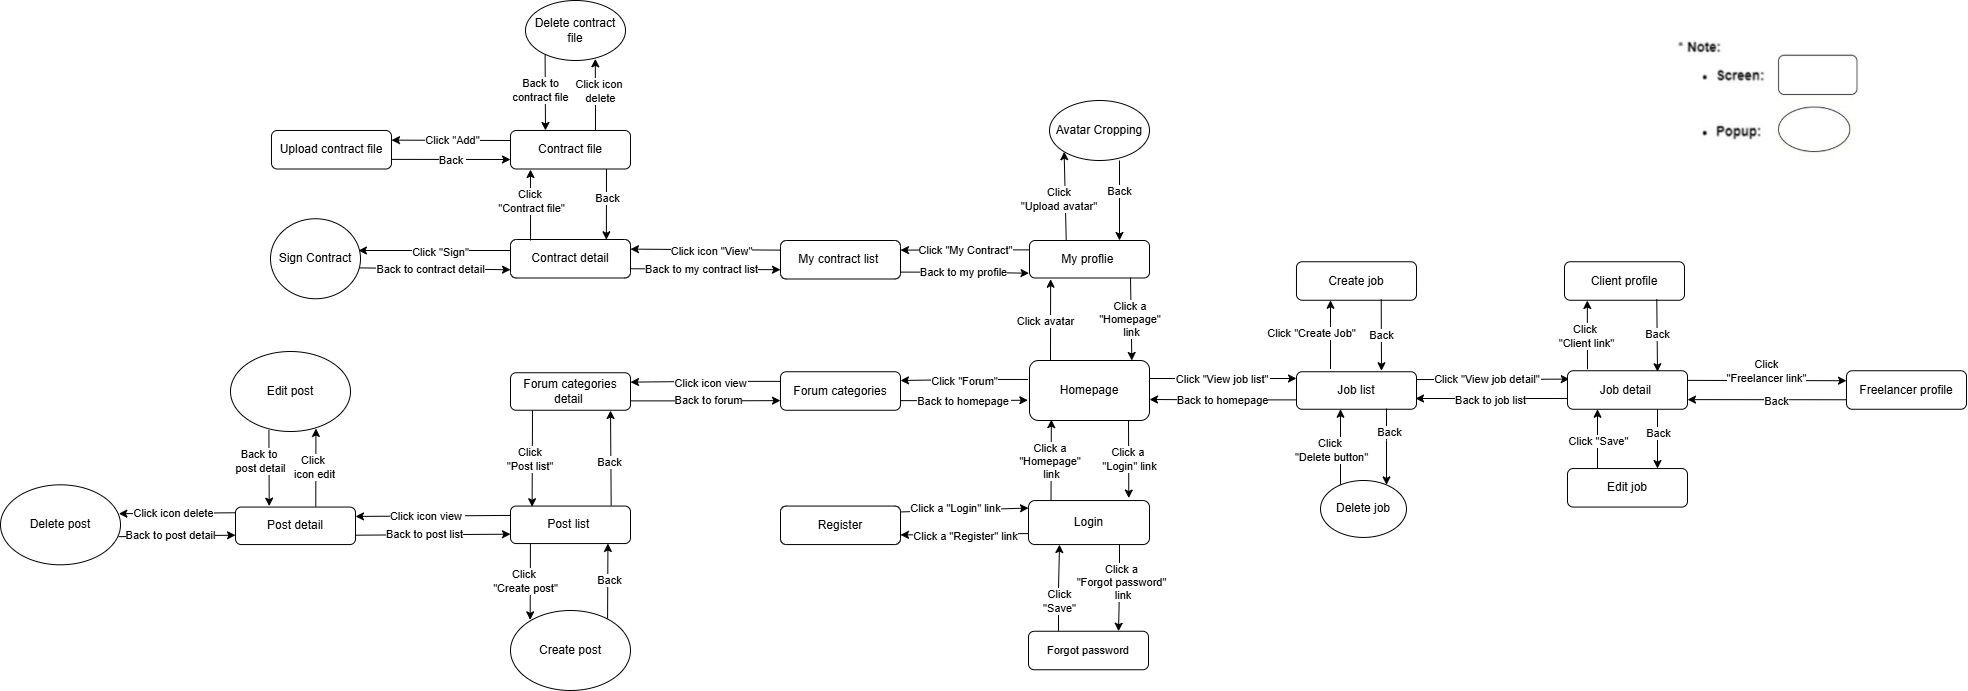
\includegraphics[width=\linewidth]{image/Screen_flow/Screen_flow_for_client.drawio.png}
    \caption{Screen Flow of Client}
    \label{fig:screenflowclient}
\end{figure}

\begin{figure}[H] % Sửa htbp thành H
    \centering
    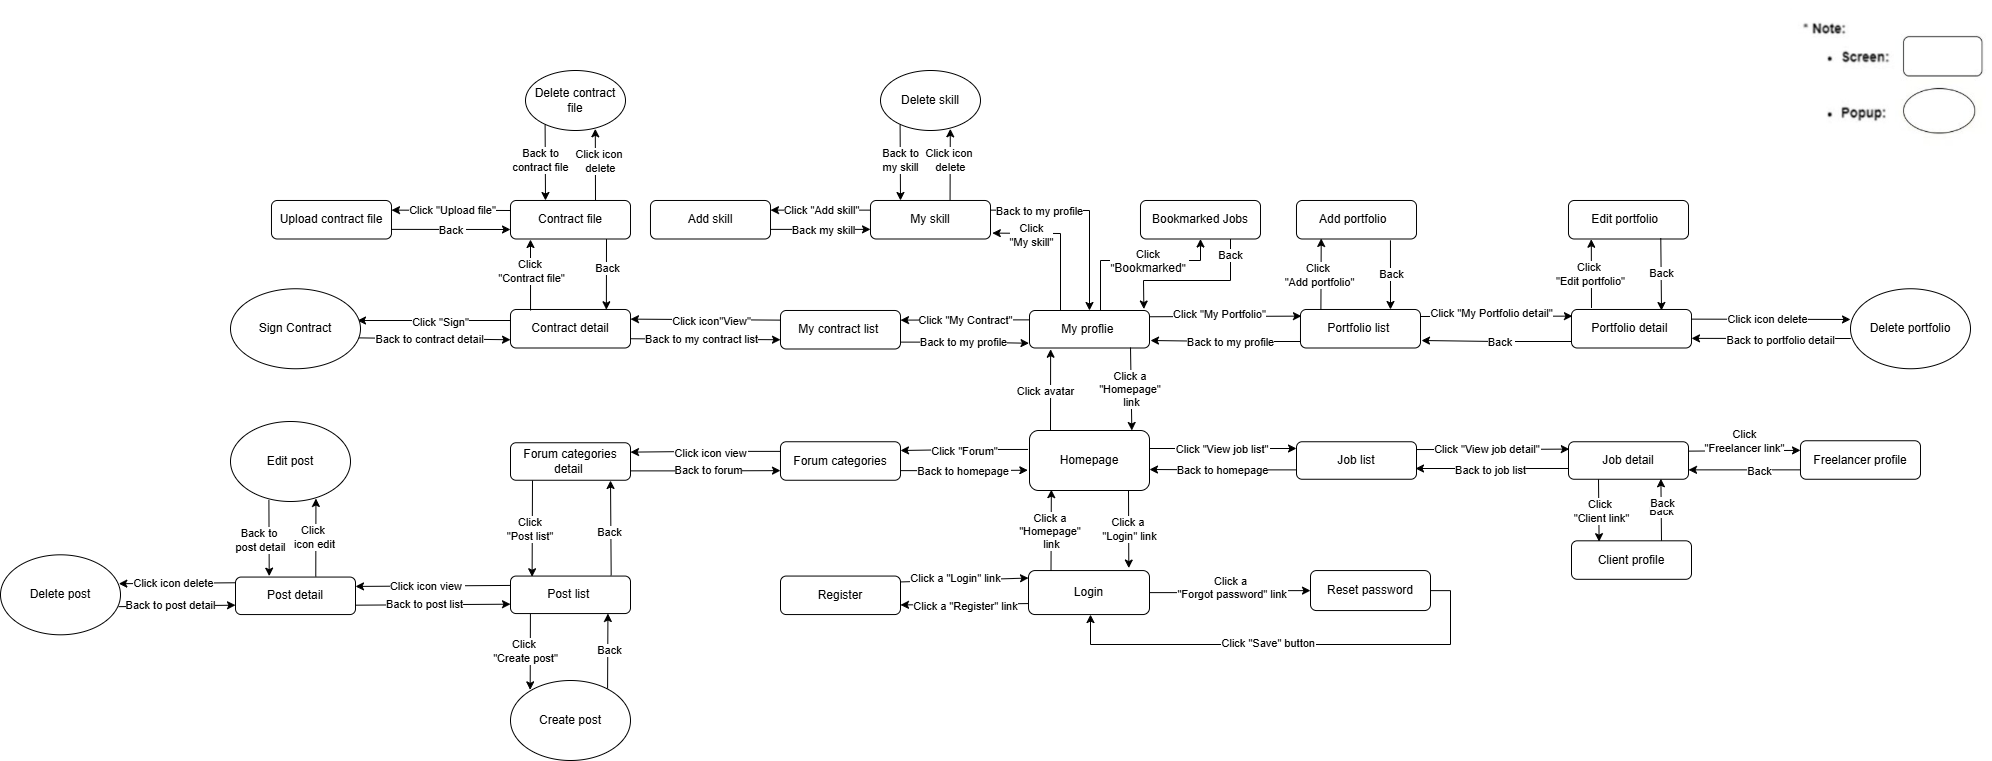
\includegraphics[width=\linewidth]{image/Screen_flow/Screen_flow_for_freelancer.drawio.png}
    \caption{Screen Flow of Freelancer}
    \label{fig:screenflowfreelancer}
\end{figure}

\begin{figure}[H] % Sửa htbp thành H
    \centering
    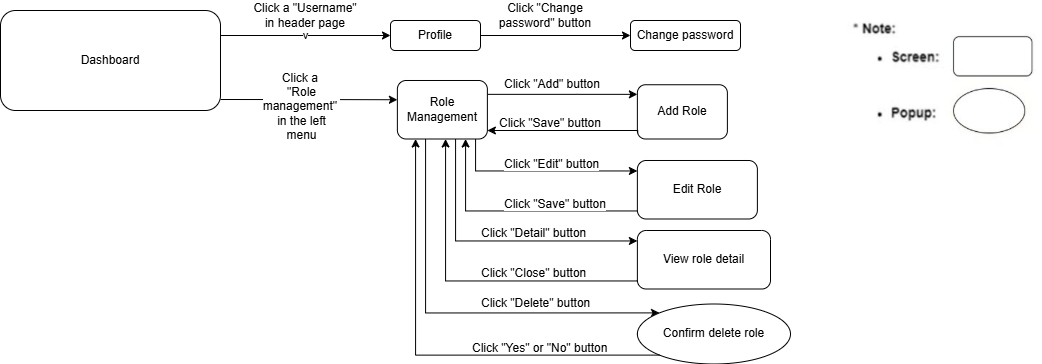
\includegraphics[width=\linewidth]{image/Screen_flow/Screen_flow_for_admin.drawio.png}
    \caption{Screen Flow of Admin}
    \label{fig:screenflowadmin}
\end{figure}

\begin{figure}[H] % Sửa htbp thành H
    \centering
    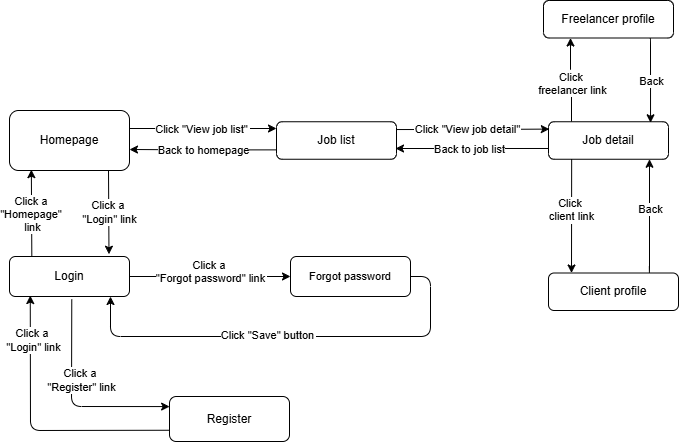
\includegraphics[width=\linewidth]{image/Screen_flow/Screen_flow_for_guest.drawio.png}
    \caption{Screen Flow of Guest}
    \label{fig:screenflowguest}
\end{figure}

% Ngắt trang bắt buộc để phần Bảng bên dưới sang trang mới sạch sẽ, không bị dính vào ảnh
\clearpage

\subsubsection{Screen Details}
\renewcommand{\arraystretch}{1.3}
\begin{longtable}{|c|>{\centering\arraybackslash}m{2.5cm}|p{3.5cm}|p{6cm}|}
\hline
\rowcolor{headerbg}
\textbf{No} &
\textbf{Actor} &
\textbf{Screen Name} &
\textbf{Description} \\
\hline
\endfirsthead
\hline
\rowcolor{headerbg}
\textbf{No} &
\textbf{Actor} &
\textbf{Screen Name} &
\textbf{Description} \\
\hline
\endhead
\hline
\endfoot
\hline
\endlastfoot
% ==========================================================
% Guest
% ==========================================================
1 &
\multirow{8}{2.5cm}{\centering Guest} &
Homepage &
The main landing page introducing the platform and its features.
\\ \cline{1-1}\cline{3-4}
2 &
&
Login &
Allows users to log in using email/password and JWT authentication.
\\ \cline{1-1}\cline{3-4}
3 &
&
Forgot Password &
Allows users to request a password reset via email verification link.
\\ \cline{1-1}\cline{3-4}
4 &
&
Register &
Allows users to create new accounts using email and password.
\\ \cline{1-1}\cline{3-4}
5 &
&
Job List &
Displays a list of available jobs with search and filter capabilities.
\\ \cline{1-1}\cline{3-4}
6 &
&
Job Detail &
Displays full details of a specific job posting.
\\ \cline{1-1}\cline{3-4}
7 &
&
Freelancer Profile &
Displays a freelancer's public profile including skills and portfolio.
\\ \cline{1-1}\cline{3-4}
8 &
&
Client Profile &
Displays a client's public profile including posted jobs and reviews.
\\ \hline
% ==========================================================
% Freelancer
% ==========================================================
9 &
\multirow{28}{2.5cm}{\centering Freelancer} &
Google Login &
Allows users to login/register using Google OAuth.
\\ \cline{1-1}\cline{3-4}
10 &
&
Login &
Allows users to log in using email/password and JWT authentication.
\\ \cline{1-1}\cline{3-4}
11 &
&
Logout &
Allows users to logout and terminate authentication session.
\\ \cline{1-1}\cline{3-4}
12 &
&
Register &
Allows users to create new accounts using email and password.
\\ \cline{1-1}\cline{3-4}
13 &
&
Forgot Password &
Allows users to request password reset via email verification link.
\\ \cline{1-1}\cline{3-4}
14 &
&
My Profile &
Main dashboard for freelancer to manage their skills, contracts, and portfolio.
\\ \cline{1-1}\cline{3-4}
15 &
&
My Skill &
Displays the list of skills added by the freelancer.
\\ \cline{1-1}\cline{3-4}
16 &
&
Add Skill &
Form screen to add a new skill to the profile.
\\ \cline{1-1}\cline{3-4}
17 &
&
Delete Skill &
Popup dialog to confirm the deletion of a skill.
\\ \cline{1-1}\cline{3-4}
18 &
&
Bookmarked Jobs &
Displays a list of jobs that the freelancer has bookmarked or saved.
\\ \cline{1-1}\cline{3-4}
19 &
&
My Contract List &
Displays all active and past contracts associated with the freelancer.
\\ \cline{1-1}\cline{3-4}
20 &
&
Contract Detail &
Displays detailed information and terms of a specific contract.
\\ \cline{1-1}\cline{3-4}
21 &
&
Sign Contract &
Popup/Action screen allowing the freelancer to digitally sign a contract.
\\ \cline{1-1}\cline{3-4}
22 &
&
Contract File &
Displays documents and files attached to a specific contract.
\\ \cline{1-1}\cline{3-4}
23 &
&
Upload Contract File &
Form screen to upload new files or documents to a contract.
\\ \cline{1-1}\cline{3-4}
24 &
&
Delete Contract File &
Popup dialog to confirm the deletion of a contract file.
\\ \cline{1-1}\cline{3-4}
25 &
&
Portfolio List &
Displays a list of projects and works in the freelancer's portfolio.
\\ \cline{1-1}\cline{3-4}
26 &
&
Add Portfolio &
Form screen to create and add a new project to the portfolio.
\\ \cline{1-1}\cline{3-4}
27 &
&
Portfolio Detail &
Displays full details, descriptions, and media of a specific portfolio project.
\\ \cline{1-1}\cline{3-4}
28 &
&
Edit Portfolio &
Form screen to update or modify an existing portfolio project.
\\ \cline{1-1}\cline{3-4}
29 &
&
Delete Portfolio &
Popup dialog to confirm the deletion of a portfolio project.
\\ \cline{1-1}\cline{3-4}
30 &
&
Forum Categories &
Displays a list of available discussion categories in the forum.
\\ \cline{1-1}\cline{3-4}
31 &
&
Forum Categories Detail &
Displays sub-topics and general information of a selected forum category.
\\ \cline{1-1}\cline{3-4}
32 &
&
Post List &
Displays a list of discussion threads or posts within a category.
\\ \cline{1-1}\cline{3-4}
33 &
&
Create Post &
Form screen allowing the freelancer to create a new forum post.
\\ \cline{1-1}\cline{3-4}
34 &
&
Post Detail &
Displays the full content of a forum post along with its replies.
\\ \cline{1-1}\cline{3-4}
35 &
&
Edit Post &
Form/Popup to edit the content of an existing forum post.
\\ \cline{1-1}\cline{3-4}
36 &
&
Delete Post &
Popup dialog to confirm the deletion of a forum post.
\\ \hline
% ==========================================================
% Client
% ==========================================================
37 &
\multirow{20}{2.5cm}{\centering Client} &
Google Login &
Allows users to login/register using Google OAuth.
\\ \cline{1-1}\cline{3-4}
38 &
&
Login &
Allows users to log in using email/password and JWT authentication.
\\ \cline{1-1}\cline{3-4}
39 &
&
Logout &
Allows users to logout and terminate authentication session.
\\ \cline{1-1}\cline{3-4}
40 &
&
Register &
Allows users to create new accounts using email and password.
\\ \cline{1-1}\cline{3-4}
41 &
&
Forgot Password &
Allows users to request password reset via email verification link.
\\ \cline{1-1}\cline{3-4}
42 &
&
Client Dashboard &
Main dashboard for authenticated clients, showing active jobs, contract summaries, and notifications.
\\ \cline{1-1}\cline{3-4}
43 &
&
Create Job Form &
Form screen allowing clients to create and publish a new job posting with details (title, description, budget, category, skills).
\\ \cline{1-1}\cline{3-4}
44 &
&
Edit Job &
Form screen allowing clients to modify details of an existing job posting.
\\ \cline{1-1}\cline{3-4}
45 &
&
Delete Job &
Popup dialog to confirm the soft deletion of a job posting.
\\ \cline{1-1}\cline{3-4}
46 &
&
Change Job Status &
Form/Dropdown action to change the status of a job posting (Open, In Progress, Closed, Cancelled).
\\ \cline{1-1}\cline{3-4}
47 &
&
My Contract List &
Displays all active and past contracts associated with the client.
\\ \cline{1-1}\cline{3-4}
48 &
&
Contract Detail &
Work interface for client to manage contract terms, milestones, and release escrow payments.
\\ \cline{1-1}\cline{3-4}
49 &
&
Create Contract &
Form screen allowing the client to initiate and create a new contract with a freelancer.
\\ \cline{1-1}\cline{3-4}
50 &
&
Update Contract Terms &
Form/Edit screen to update terms, milestones, and payment settings of a pending contract.
\\ \cline{1-1}\cline{3-4}
51 &
&
Sign Contract &
Popup/Action screen allowing the client to digitally sign and fund the contract escrow (Web3).
\\ \cline{1-1}\cline{3-4}
52 &
&
Cancel Contract &
Popup/Action screen allowing the client to request contract cancellation and handle escrow refunds.
\\ \cline{1-1}\cline{3-4}
53 &
&
Upload Contract File &
Form screen allowing the client to upload files or deliverables to a contract.
\\ \cline{1-1}\cline{3-4}
54 &
&
Delete Contract File &
Popup dialog to confirm the deletion of a contract file.
\\ \cline{1-1}\cline{3-4}
55 &
&
View Progress Updates &
Screen displaying progress updates and attached proof of work submitted by the freelancer.
\\ \cline{1-1}\cline{3-4}
56 &
&
Hired Freelancers &
Screen displaying the list of freelancers currently hired by the client.
\\ \hline
% ==========================================================
% Admin
% ==========================================================
57 &
\multirow{8}{2.5cm}{\centering Admin} &
Dashboard &
Main admin screen displaying system overview and key statistics.
\\ \cline{1-1}\cline{3-4}
58 &
&
Profile &
Allows admin to view and update personal account information.
\\ \cline{1-1}\cline{3-4}
59 &
&
Change Password &
Allows admin to change their account password.
\\ \cline{1-1}\cline{3-4}
60 &
&
Role Management &
Displays a list of all roles along with their assigned permissions.
\\ \cline{1-1}\cline{3-4}
61 &
&
Add Role &
Form screen for creating a new role with name, description, and permissions.
\\ \cline{1-1}\cline{3-4}
62 &
&
Edit Role &
Form screen for modifying an existing role's name, description, and permissions.
\\ \cline{1-1}\cline{3-4}
63 &
&
View Role Detail &
Displays detailed information of a specific role including its permissions.
\\ \cline{1-1}\cline{3-4}
64 &
&
Confirm Delete Role &
Popup dialog prompting admin to confirm before permanently deleting a role.
\\ \hline
\end{longtable}


\subsubsection{Screen Authorization}

\renewcommand{\arraystretch}{1.3}

\begin{longtable}{|c|p{5.2cm}|c|c|c|c|}

% Đầu bảng (lặp lại ở mỗi trang)
\hline
\rowcolor{headerbg}
\multicolumn{1}{|c|}{\textbf{No}} &
\multicolumn{1}{c|}{\textbf{Screen / Page}} &
\multicolumn{1}{c|}{\textbf{Guest}} &
\multicolumn{1}{c|}{\textbf{Client}} &
\multicolumn{1}{c|}{\textbf{Freelancer}} &
\multicolumn{1}{c|}{\textbf{Admin}}
\\ \hline
\endfirsthead

% Đầu bảng cho các trang tiếp theo
\hline
\rowcolor{headerbg}
\multicolumn{1}{|c|}{\textbf{No}} &
\multicolumn{1}{c|}{\textbf{Screen / Page}} &
\multicolumn{1}{c|}{\textbf{Guest}} &
\multicolumn{1}{c|}{\textbf{Client}} &
\multicolumn{1}{c|}{\textbf{Freelancer}} &
\multicolumn{1}{c|}{\textbf{Admin}}
\\ \hline
\endhead

\endfoot

% Chân bảng cuối cùng
\hline
\endlastfoot

% Nội dung bảng (50 dòng)
1 & Forum Categories & \checkmark & \checkmark & \checkmark & \checkmark \\ \hline
2 & Forum Category Detail & \checkmark & \checkmark & \checkmark & \checkmark \\ \hline
3 & Post List & \checkmark & \checkmark & \checkmark & \checkmark \\ \hline
4 & Post Detail & \checkmark & \checkmark & \checkmark & \checkmark \\ \hline
5 & View Comments & \checkmark & \checkmark & \checkmark & \checkmark \\ \hline
6 & View Comment Detail & \checkmark & \checkmark & \checkmark & \checkmark \\ \hline
7 & Create Post & & \checkmark & \checkmark &  \\ \hline
8 & Edit Post & & \checkmark & \checkmark &  \\ \hline
9 & Delete Post & & \checkmark & \checkmark & \checkmark \\ \hline
10 & Like Post & & \checkmark & \checkmark & \\ \hline
11 & Unlike Post & & \checkmark & \checkmark & \\ \hline
12 & Add Comment & & \checkmark & \checkmark &  \\ \hline
13 & Edit Comment & & \checkmark & \checkmark &  \\ \hline
14 & Delete Comment & & \checkmark & \checkmark & \checkmark \\ \hline
15 & Like Comment & & \checkmark & \checkmark & \\ \hline
16 & Unlike Comment & & \checkmark & \checkmark & \\ \hline
17 & Report Content & & \checkmark & \checkmark & \\ \hline
18 & View Detailed Freelancer Profile & \checkmark & \checkmark & \checkmark & \\ \hline

19 & Update Detailed Freelancer Profile & & & \checkmark & \\ \hline

20 & Get List Freelancer Skill & \checkmark & \checkmark & \checkmark & \\ \hline

21 & Add Freelancer Skill & & & \checkmark & \\ \hline

22 & Delete Freelancer Skill & & & \checkmark & \\ \hline

23 & Get Portfolio List & & & \checkmark & \\ \hline

24 & Add New Portfolio & & & \checkmark & \\ \hline

25 & Get Portfolio Detail & & & \checkmark & \\ \hline

26 & Update Portfolio & & & \checkmark & \\ \hline

27 & Delete Portfolio & & & \checkmark & \\ \hline
28 & Create Contract & & \checkmark & & \\ \hline
29 & Update Contract Terms & & \checkmark & & \\ \hline
30 & Complete Contract & & \checkmark & \checkmark & \\ \hline
31 & Get Contract List & & \checkmark & \checkmark & \checkmark \\ \hline
32 & Get Contract Detail & & \checkmark & \checkmark & \checkmark \\ \hline
33 & Sign Contract & & \checkmark & \checkmark & \\ \hline
34 & Cancel Contract & & \checkmark & \checkmark & \checkmark \\ \hline
35 & Contract Activities & & \checkmark & \checkmark & \checkmark \\ \hline
36 & Contract Files & & \checkmark & \checkmark & \checkmark \\ \hline
37 & Upload Contract File & & \checkmark & \checkmark & \\ \hline
38 & Delete Contract File & & \checkmark & \checkmark & \checkmark \\ \hline
39 & Progress Update & & & \checkmark & \\ \hline
40 & View Progress Updates & & \checkmark & \checkmark & \checkmark \\ \hline
41 & Google Login & \checkmark & & & \\ \hline
42 & Login & \checkmark & & & \\ \hline
43 & Logout & & \checkmark & \checkmark & \checkmark \\ \hline
44 & Register & \checkmark & & & \\ \hline
45 & Forgot Password & \checkmark & \checkmark & \checkmark & \checkmark \\ \hline
46 & View Role List & & & & \checkmark \\ \hline
47 & View Role Detail & & & & \checkmark \\ \hline
48 & Create New Role & & & & \checkmark \\ \hline
49 & Update Role & & & & \checkmark \\ \hline
50 & Delete Role & & & & \checkmark \\ \hline
51 & View List Job & \checkmark & \checkmark & \checkmark &  \\ \hline
52 & View Job Detail & \checkmark & \checkmark & \checkmark &  \\ \hline
53 & Post New Job & & \checkmark & &  \\ \hline
54 & Edit Job & & \checkmark & &  \\ \hline
55 & Delete Job & & \checkmark & &  \\ \hline
56 & Change Job Status & & \checkmark & &  \\ \hline
57 & View List Bookmarked Job & & & \checkmark &  \\ \hline
58 & Bookmark Job & & & \checkmark &  \\ \hline
59 & Remove Bookmark & & & \checkmark & 
\label{tab:screen_authorization}
\end{longtable}

\subsubsection{Non-Screen Functions}

\renewcommand{\arraystretch}{1.4}

\begin{longtable}{|C{0.8cm}|L{2.8cm}|L{6.8cm}|L{5.5cm}|}
\hline
\rowcolor{headerbg}

\textbf{\#}
&
\textbf{Feature}
&
\textbf{System Function}
&
\textbf{Description}
\\ \hline
\endfirsthead

\hline
\rowcolor{headerbg}

\textbf{\#}
&
\textbf{Feature}
&
\textbf{System Function}
&
\textbf{Description}
\\ \hline
\endhead

3
&
\textbf{Manage Forum}
&
[GET] /api/forum/categories \newline
[GET] /api/forum/categories/\{id\} \newline
[GET] /api/forum/posts \newline
[GET] /api/forum/posts/\{id\} \newline
[GET] /api/forum/comments/\{postId\} \newline
[GET] /api/forum/comments/\{id\} \newline
[POST] /api/forum/posts \newline
[PUT] /api/forum/posts/\{id\} \newline
[DELETE] /api/forum/posts/\{id\} \newline
[POST] /api/forum/like-post/\{id\} \newline
[DELETE] /api/forum/unlike-post/\{id\} \newline
[POST] /api/forum/comments \newline
[PUT] /api/forum/comments/\{id\} \newline
[DELETE] /api/forum/comments/\{id\} \newline
[POST] /api/forum/like-comments/\{id\} \newline
[DELETE] /api/forum/unlike-comments/\{id\} \newline
[POST] /api/forum/report-contents
&
The Forum Management feature enables community discussion and knowledge sharing within the platform. Users can browse forum categories, view discussion threads, create and manage posts, add comments, react to content through likes, and report inappropriate content. Guests can access public forum content, while authenticated users can participate in discussions by creating posts, commenting, reacting, and reporting violations. Administrators can moderate forum activities and maintain community standards.
\\ \hline
4
&
\textbf{Manage Contract}
&
[GET] /api/contracts \newline
[GET] /api/contracts/{id} \newline
[GET] /api/contracts/{id}/files \newline
[POST] /api/contracts/{id}/files \newline
[DELETE] /api/contracts/files/{id} \newline
[POST] /api/contracts/{id}/sign \newline
[PUT] /api/contracts/{id}/terms \newline
[POST] /api/contracts/{id}/milestones/{id}/complete \newline
[POST] /api/contracts/{id}/cancel
&
The Contract Management feature enables clients to manage agreements and collaboration with freelancers throughout the project lifecycle. Users can browse contract lists, view contract details, upload and manage contract-related files, and digitally sign contracts to confirm participation. Clients can update contract terms, manage milestone execution, release escrow payments upon successful milestone completion, and request contract cancellation when necessary. The feature ensures secure transactions, transparent collaboration, and controlled contract execution between both parties. \\ \hline
5
&
\textbf{Manage Freelancer Profile}
&
[GET] /api/profiles/\{id\} \newline
[PUT] /api/profiles/\{id\} \newline
[GET] /api/profiles/\{id\}/skills \newline
[POST] /api/profiles/\{id\}/skills \newline
[DELETE] /api/profiles/skills/\{id\} \newline
[GET] /api/profiles/\{id\}/portfolios \newline
[POST] /api/profiles/\{id\}/portfolios \newline
[GET] /api/profiles/portfolios/\{id\} \newline
[PUT] /api/profiles/portfolios/\{id\} \newline
[DELETE] /api/profiles/portfolios/\{id\}
&
The Freelancer Profile Management feature enables freelancers to manage their professional identity and showcase their expertise to potential clients. Users can view and update their detailed profile information, including their bio, professional title, education, and availability status. Furthermore, freelancers can manage their skill set by adding or removing specific skills along with proficiency levels. The feature also allows freelancers to build a comprehensive portfolio by creating, updating, and deleting portfolio items with attached media files. This robust profile system helps freelancers build credibility, highlight their capabilities, and attract suitable project opportunities. \\ \hline
6
&
\textbf{Manage Freelancer Skills}
&
[GET] /api/profiles/\{id\}/skills \newline
[POST] /api/profiles/\{id\}/skills \newline
[DELETE] /api/profiles/skills/\{id\}
&
The Freelancer Skills Management feature allows freelancers to define and showcase their professional capabilities. Users can view the complete list of skills associated with a freelancer's profile, add new skills with corresponding proficiency levels (e.g., beginner, intermediate, expert), and permanently remove skills that are no longer relevant. This feature ensures that the freelancer's skill set remains accurate and up-to-date, helping clients easily evaluate their technical and professional qualifications during the talent selection process. \\ \hline
7
&
\textbf{Manage Freelancer Portfolio}
&
[GET] /api/profiles/\{id\}/portfolios \newline
[POST] /api/profiles/\{id\}/portfolios \newline
[GET] /api/profiles/portfolios/\{id\} \newline
[PUT] /api/profiles/portfolios/\{id\} \newline
[DELETE] /api/profiles/portfolios/\{id\}
&
The Freelancer Portfolio Management feature enables freelancers to visually demonstrate their past work experience and successful projects. Freelancers can create new portfolio entries by providing project details and uploading associated media files or links. The feature also allows users to view detailed information of specific portfolios, update existing portfolio content or media, and soft-delete portfolios that they no longer wish to display publicly. By maintaining a rich and organized portfolio gallery, freelancers can build stronger credibility and significantly increase their chances of being hired by prospective clients. \\ \hline
8
&
\textbf{Manage Authentication}
&
[POST] /api/auth/google \newline
[POST] /api/auth/login \newline
[POST] /api/auth/register \newline
[POST] /api/auth/forgot-password \newline
[POST] /api/auth/logout
&
The Authentication Management feature handles user identity verification and access control. It supports multiple authentication methods including traditional email/password login with JWT token generation, Google OAuth for social sign‑in, and new account registration. The feature also provides secure password reset via email verification links, and allows authenticated users to terminate their session by logging out. Together, these endpoints ensure a seamless and secure authentication experience for all platform users.
\\ \hline
9
&
\textbf{Manage Roles}
&
[GET] /api/roles \newline
[GET] /api/roles/\{id\} \newline
[POST] /api/roles \newline
[PUT] /api/roles/\{id\} \newline
[DELETE] /api/roles/\{id\}
&
The Role Management feature allows administrators to define and control user permissions within the system. Admin users can retrieve a list of all roles along with their assigned permissions, view detailed information of a specific role, create new roles with custom names and permission sets, update existing roles to modify their access rights, and delete roles that are no longer needed. This feature ensures fine‑grained access control, maintaining system security and proper segregation of duties across different user types.
\\ \hline

10
&
\textbf{Manage Job}
&
[GET] /api/jobs \newline
[GET] /api/jobs/\{id\} \newline
[POST] /api/jobs \newline
[PUT] /api/jobs/\{id\} \newline
[DELETE] /api/jobs/\{id\} \newline
[PATCH] /api/jobs/\{id\}/status \newline
[GET] /api/jobs/bookmarks \newline
[POST] /api/jobs/\{id\}/bookmark \newline
[DELETE] /api/jobs/\{id\}/bookmark
&
The Job Management feature enables clients to create and manage job postings, and allows freelancers to browse, search, and bookmark interesting opportunities. Clients can post new jobs with detailed descriptions, budgets, required skills, and timelines; edit or delete their own job postings; and update job status (Open, In Progress, Closed, Cancelled). Freelancers can view paginated job lists with filters and sorting, view full job details, and bookmark jobs for later reference. This feature serves as the core marketplace functionality connecting clients with freelancers.
\\ \hline
\end{longtable}

\subsubsection{Entity Relationship Diagram}

% ===============================================
% ERD1
% ===============================================
\paragraph{Authentication \& Role-Based Access}
\begin{figure}[H]
    \centering
    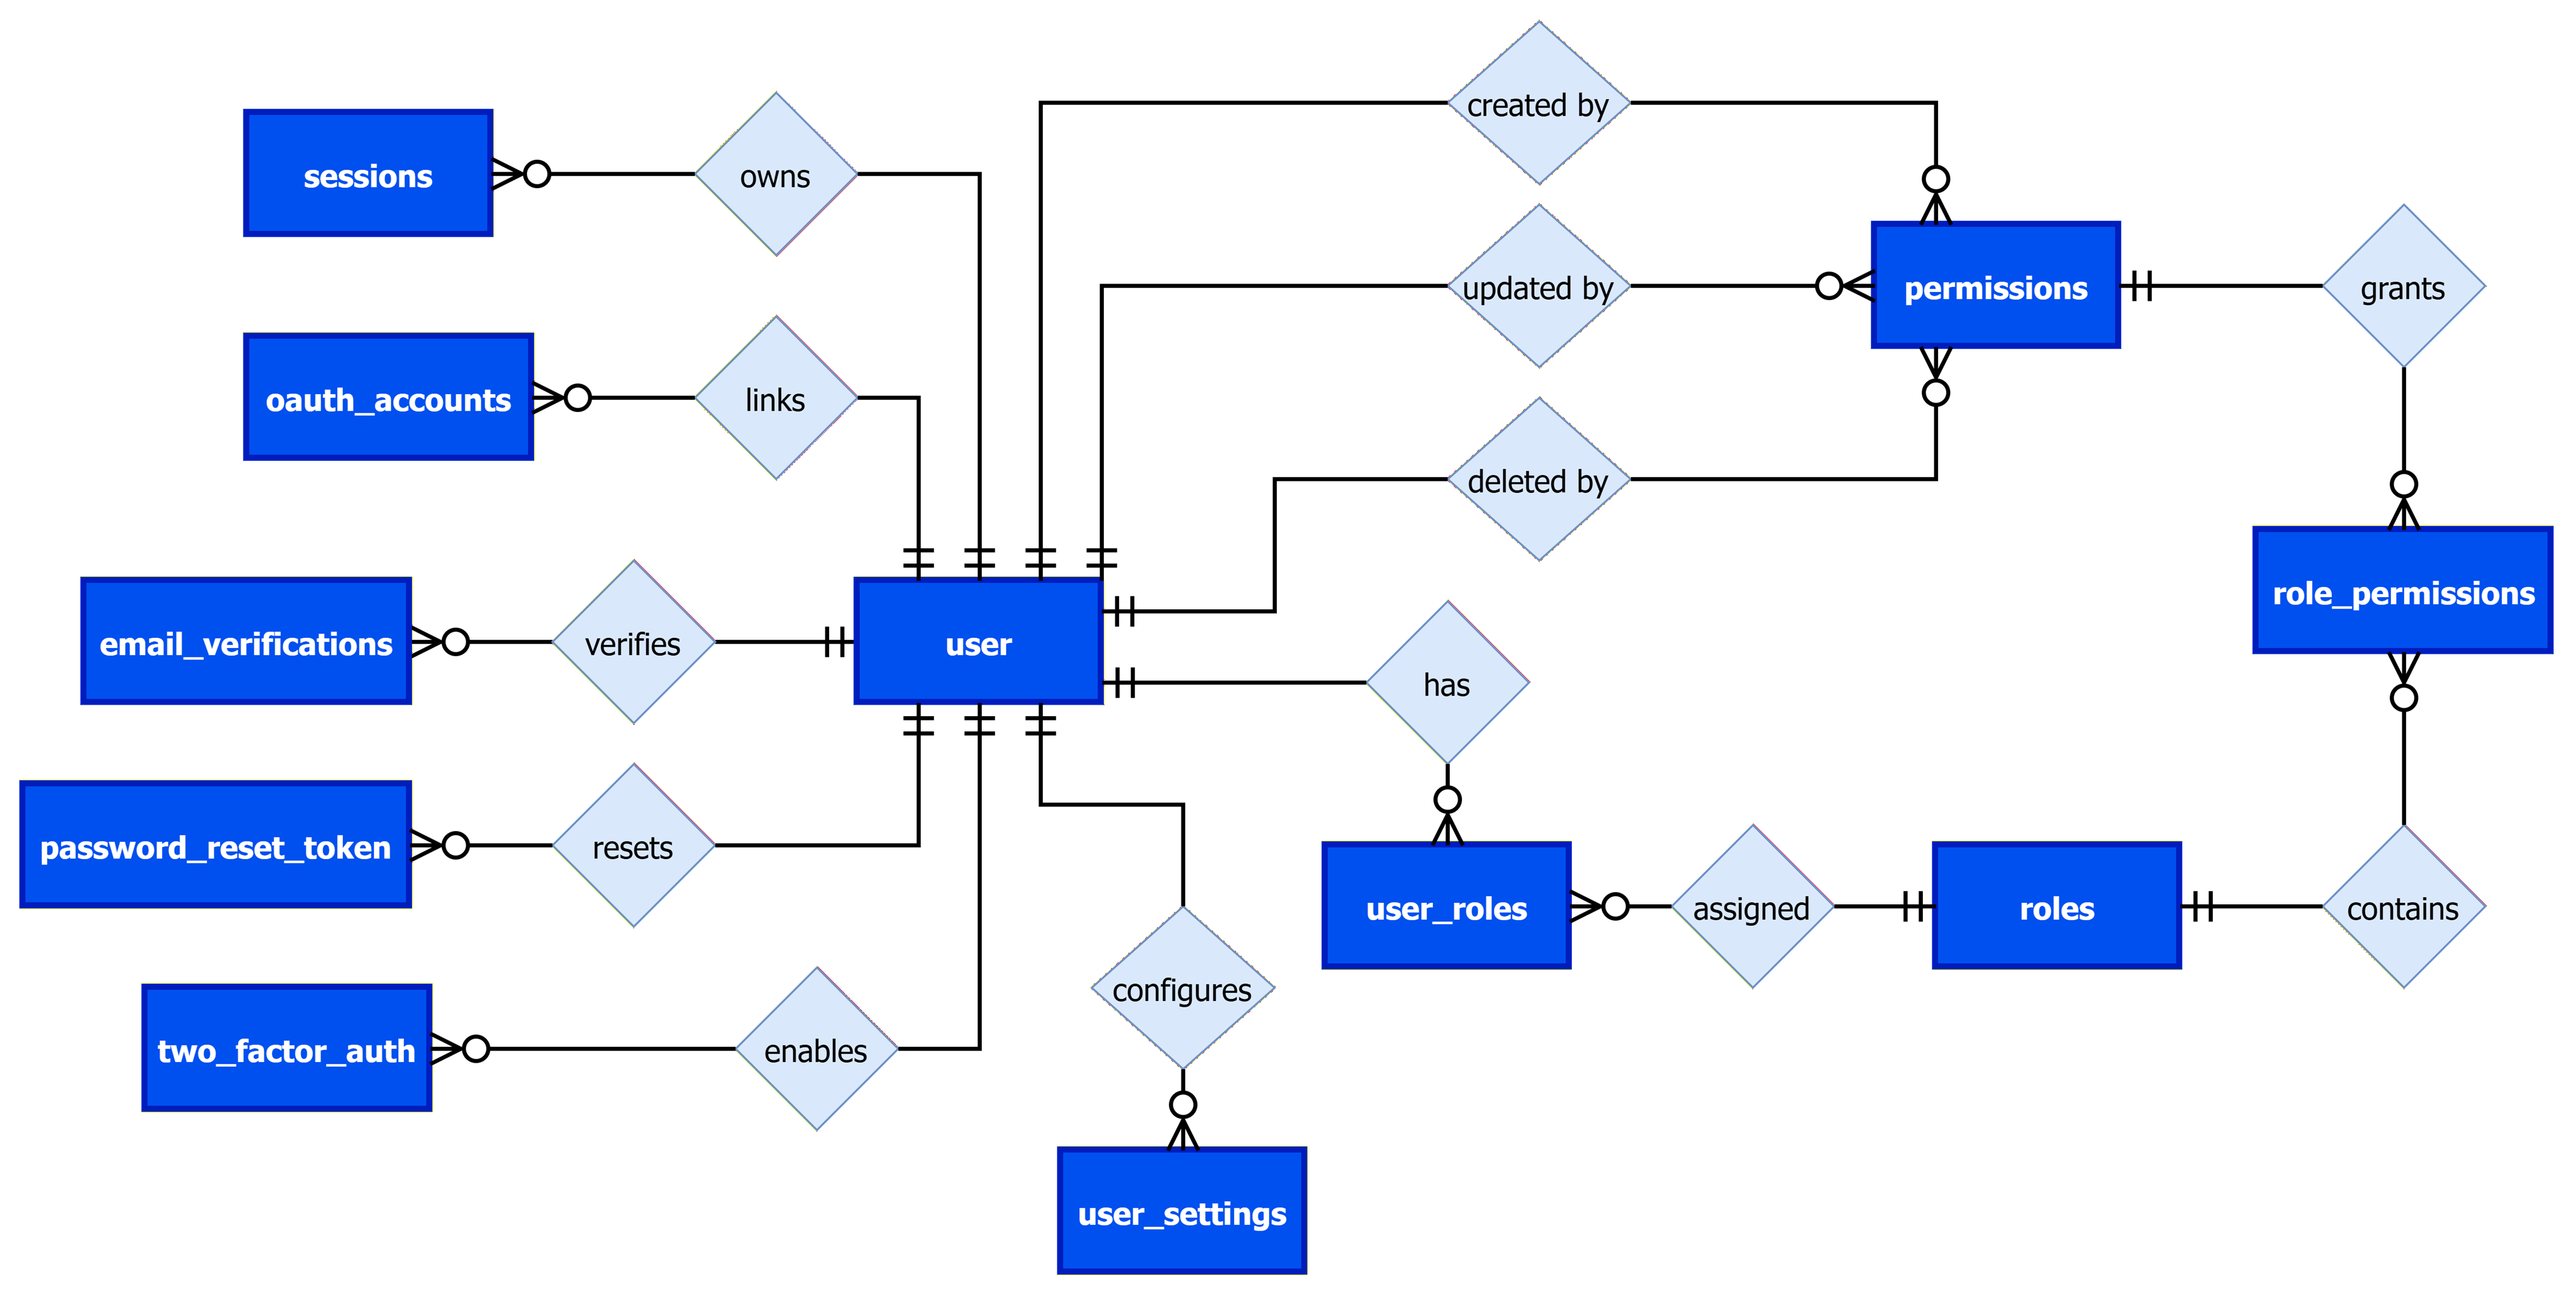
\includegraphics[width=0.95\textwidth]{image/ERD/ERD1.png}
    \caption{Authentication \& Role-Based Access ERD}
    \label{fig:authentication-role-based-access}
\end{figure}

% ===============================================
% ERD2
% ===============================================
\paragraph{Manage Profile}
\begin{figure}[H]
    \centering
    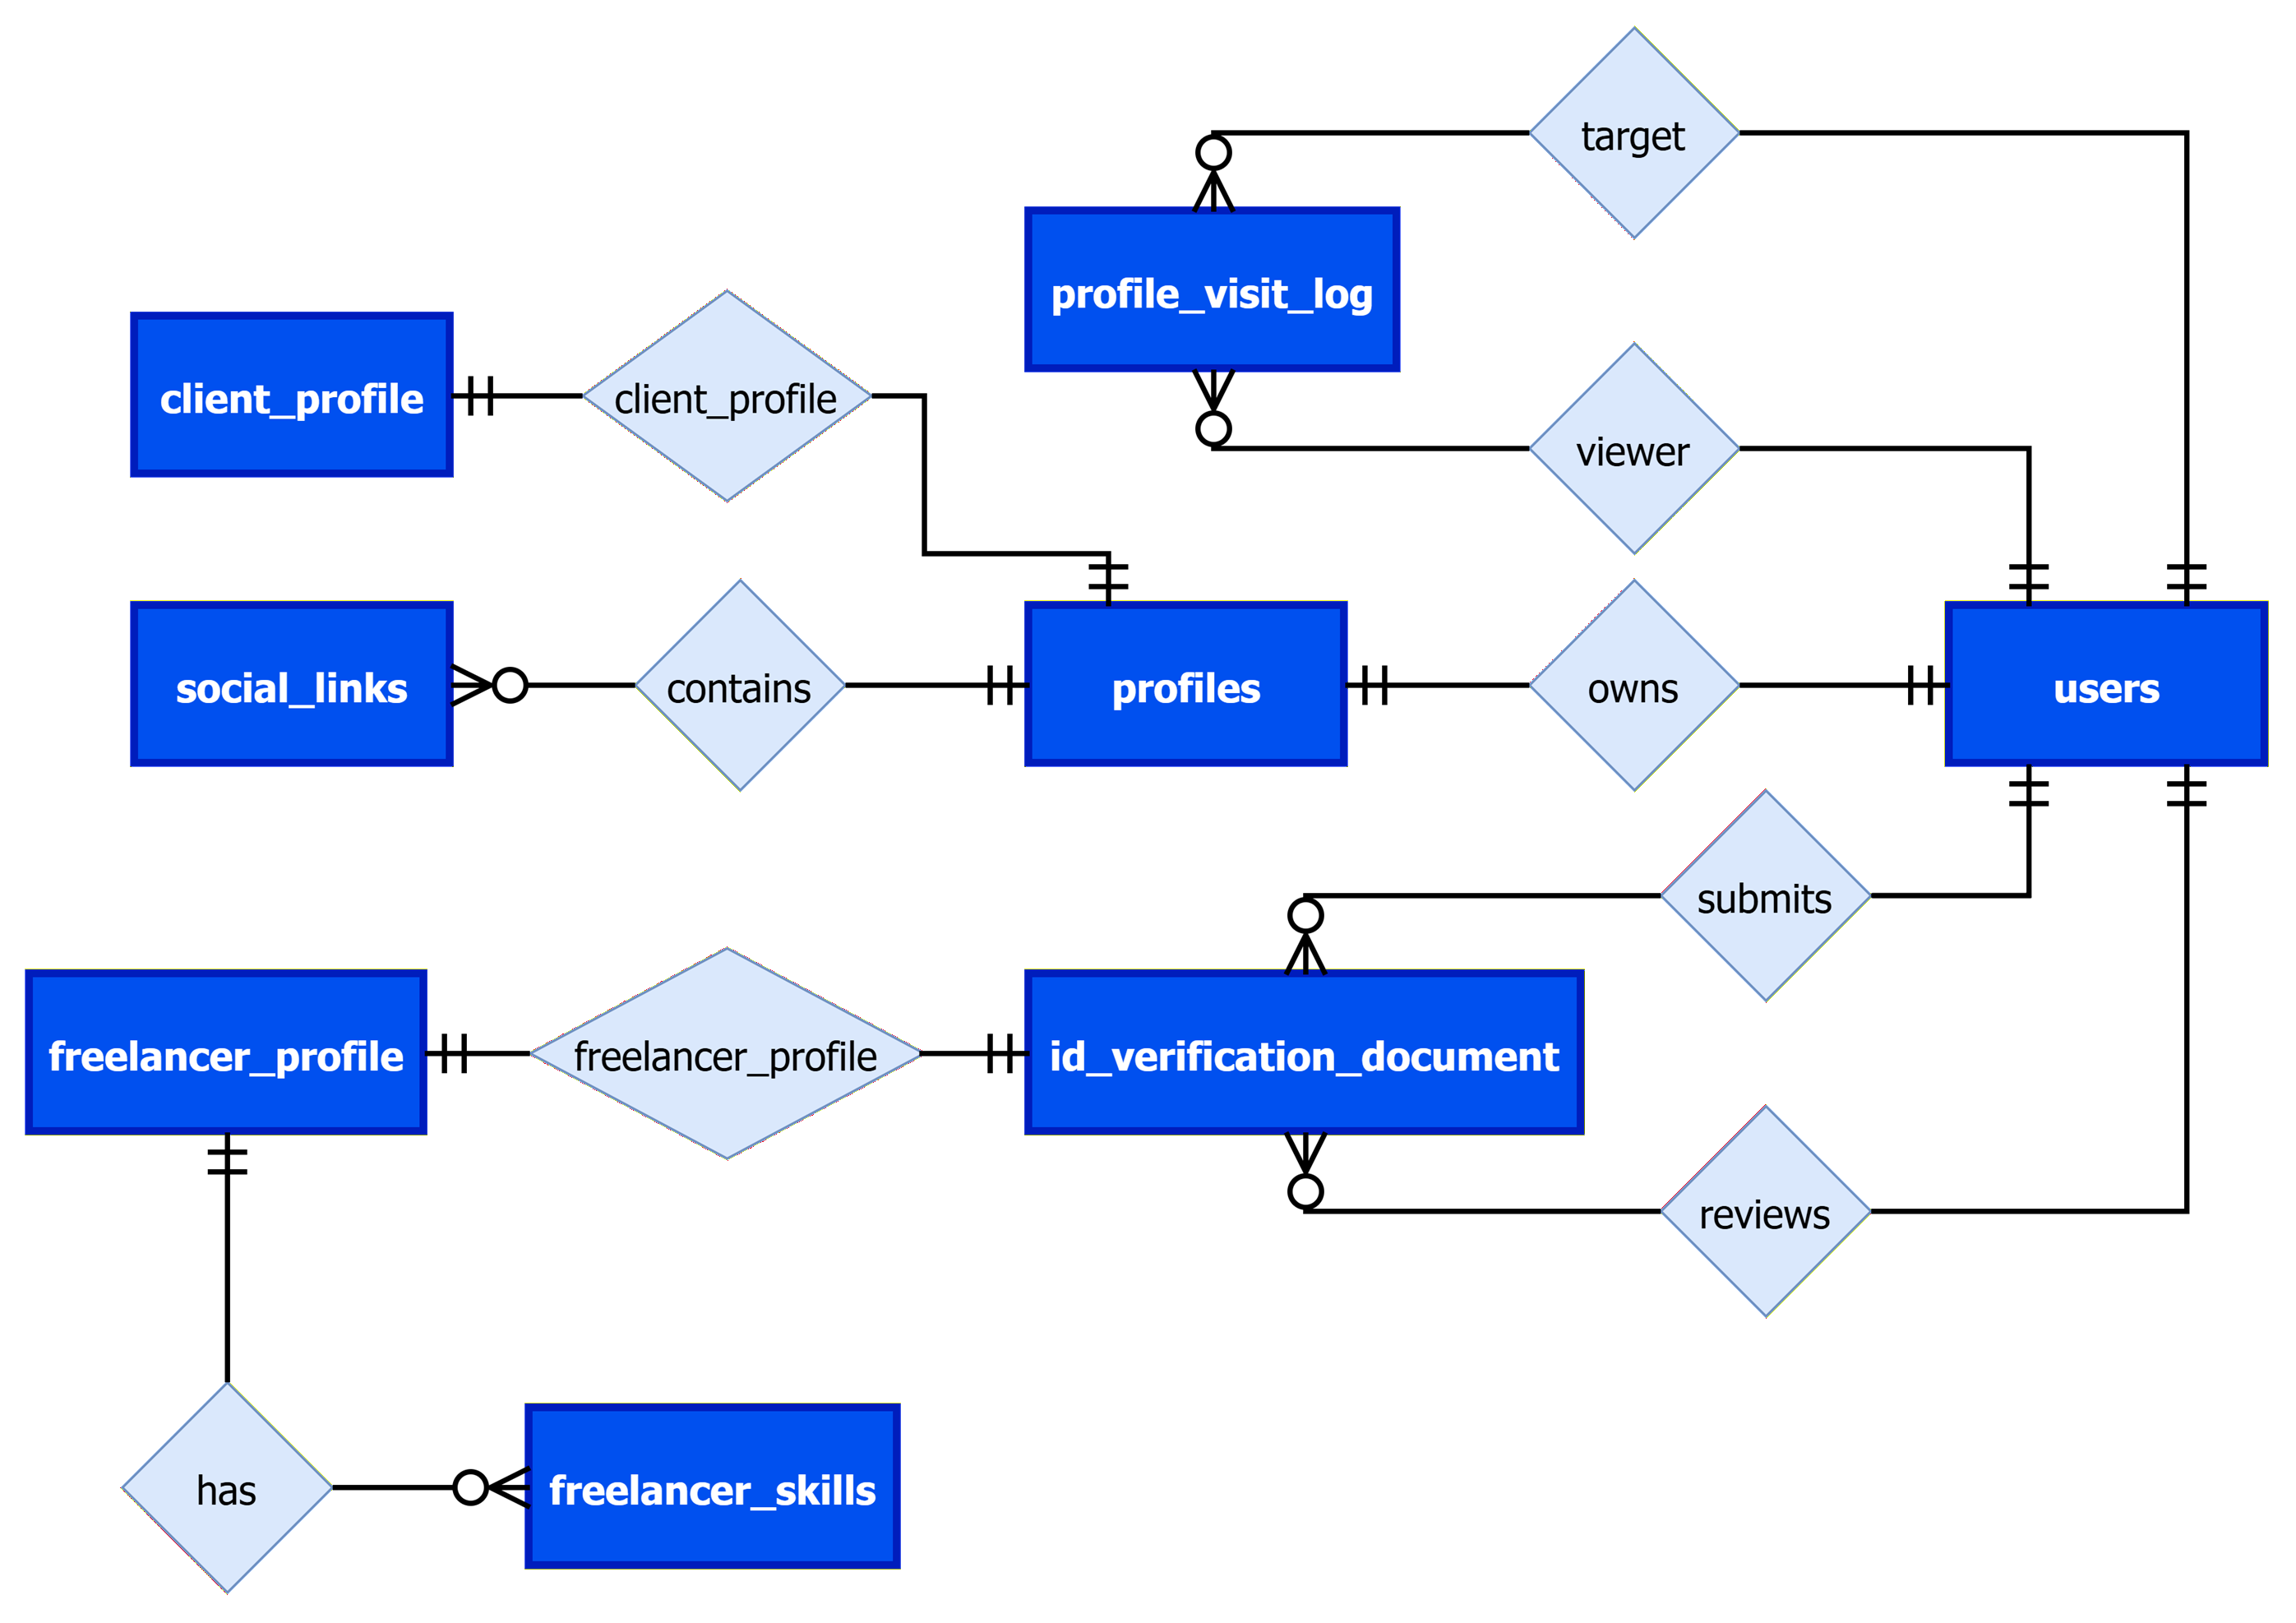
\includegraphics[width=0.95\textwidth]{image/ERD/ERD2.png}
    \caption{Manage Profile ERD}
    \label{fig:manage-profile}
\end{figure}

% ===============================================
% ERD3
% ===============================================
\paragraph{Portfolio \& Freelancer Network}
\begin{figure}[H]
    \centering
    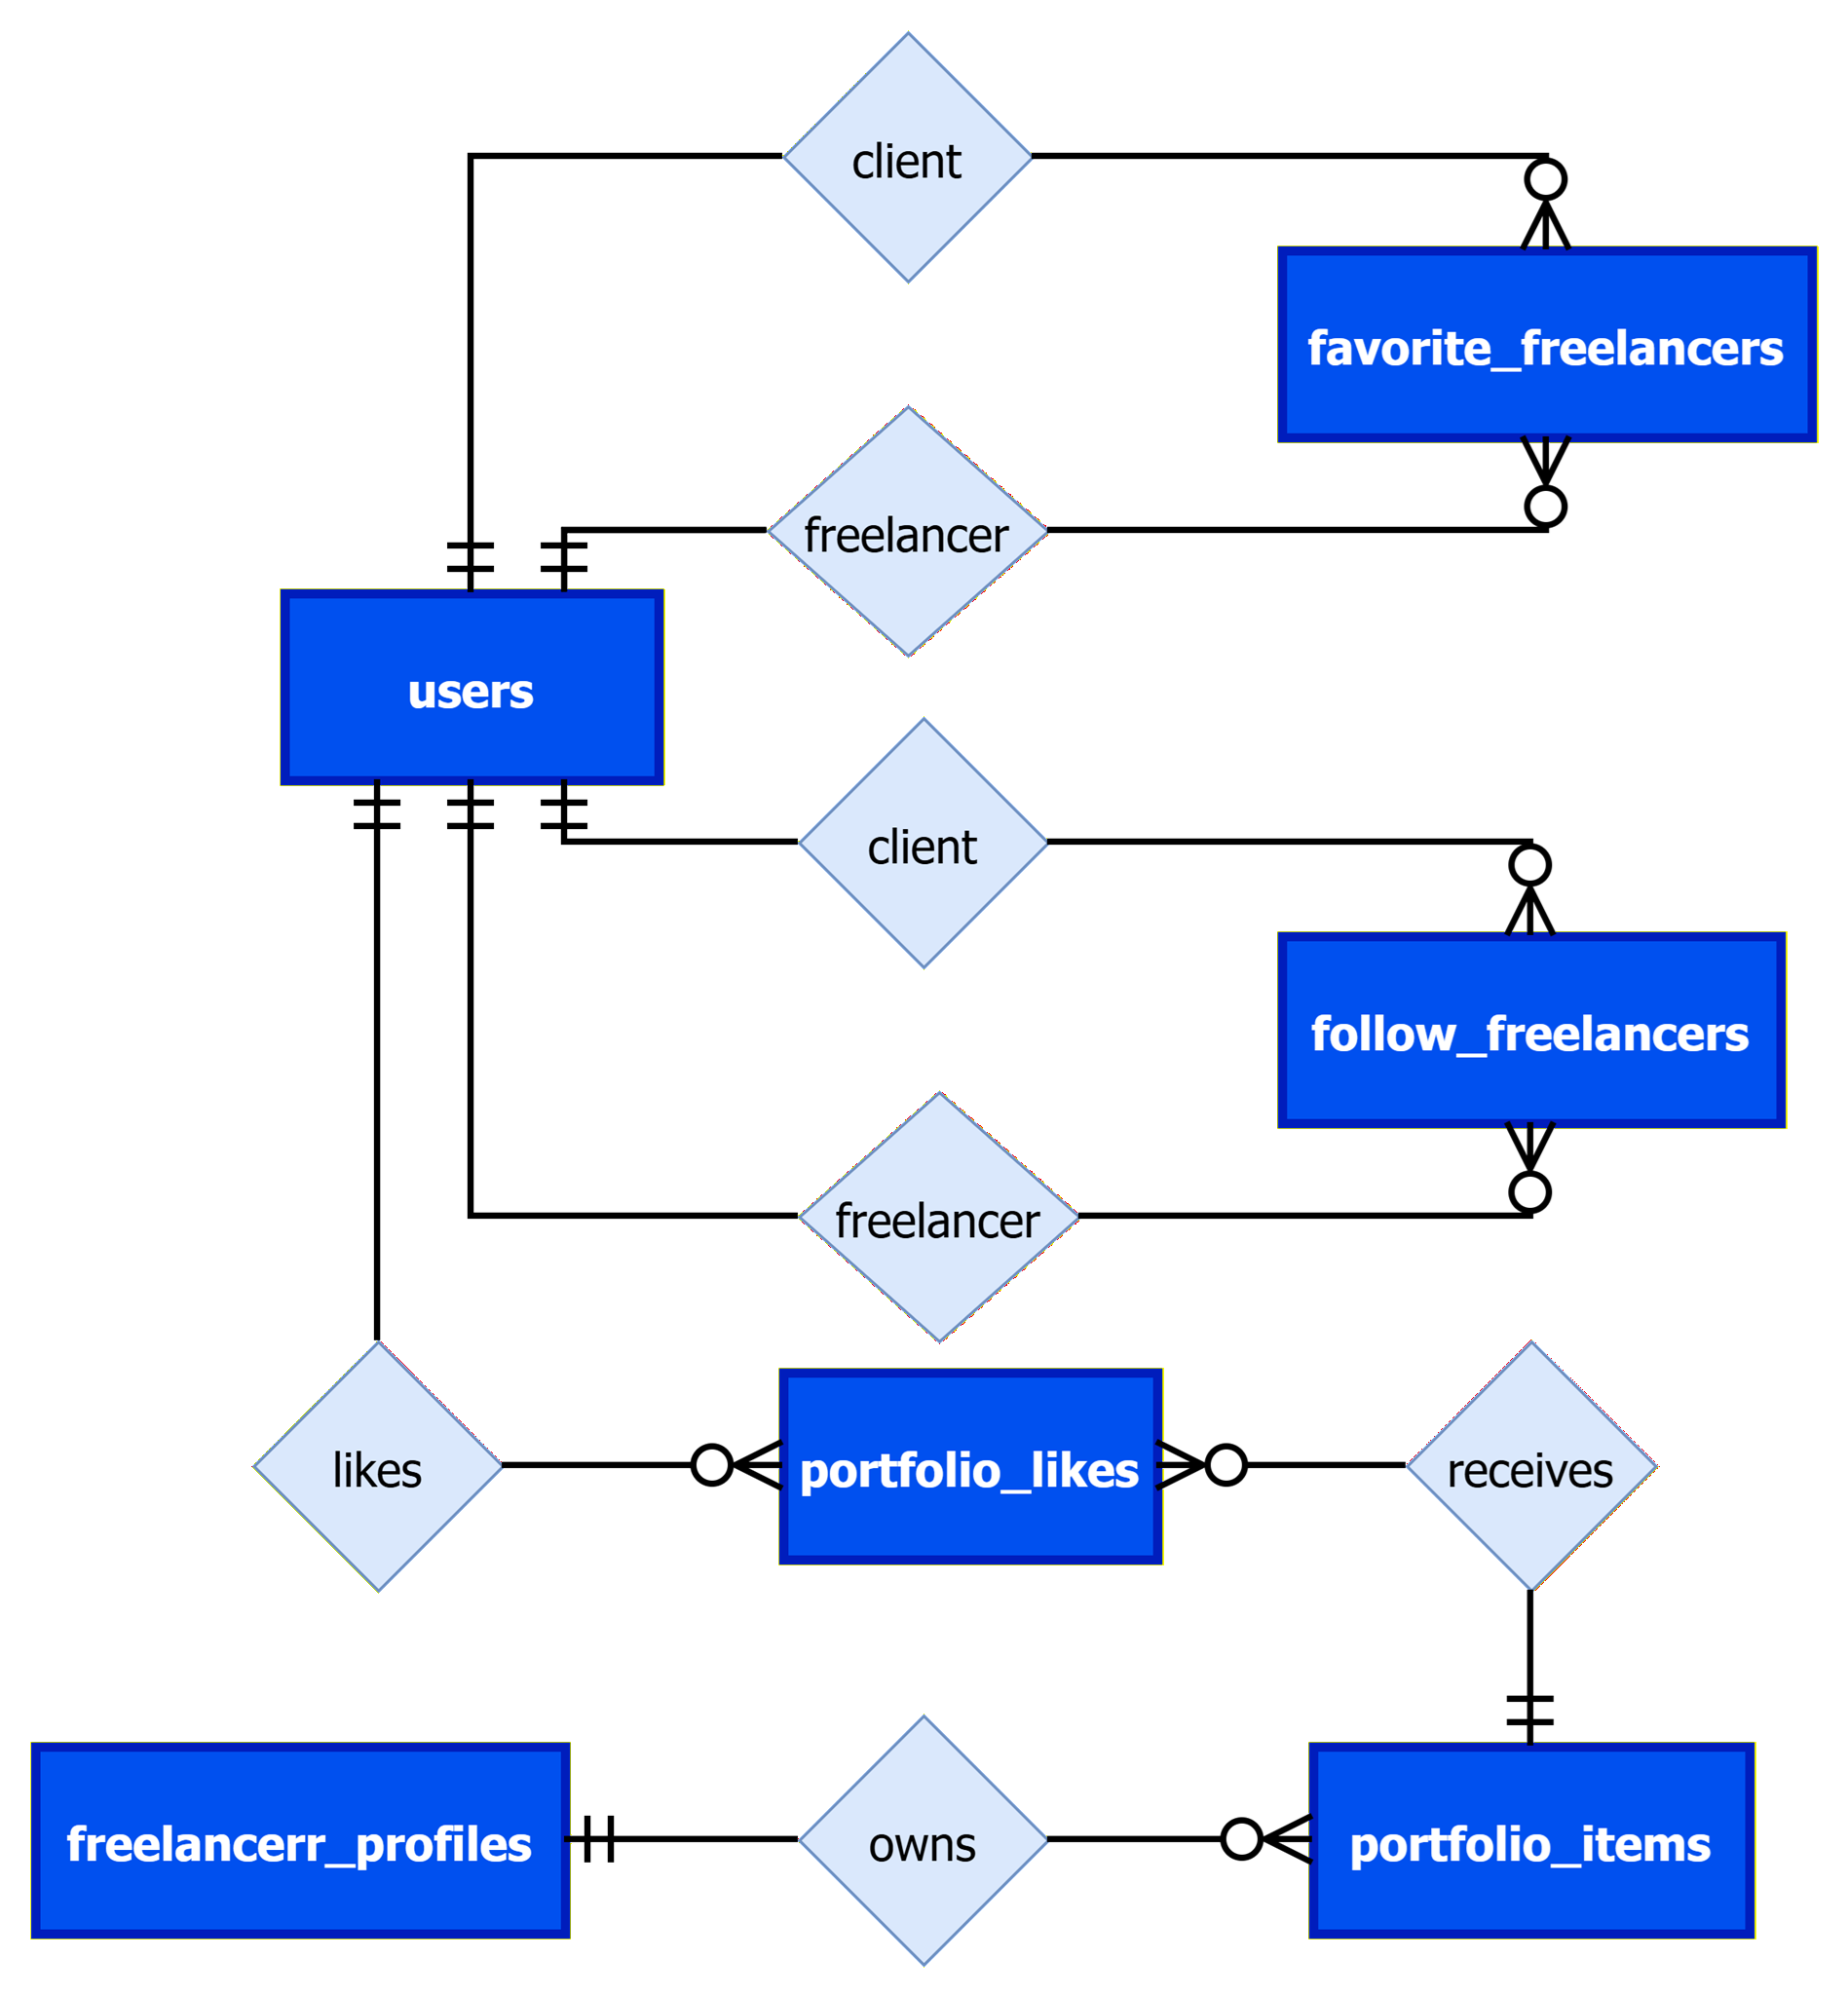
\includegraphics[width=0.95\textwidth]{image/ERD/ERD3.png}
    \caption{Portfolio \& Freelancer Network ERD}
    \label{fig:portfolio-freelancer-network}
\end{figure}

% ===============================================
% ERD4
% ===============================================
\paragraph{Job Posting \& Discovery}
\begin{figure}[H]
    \centering
    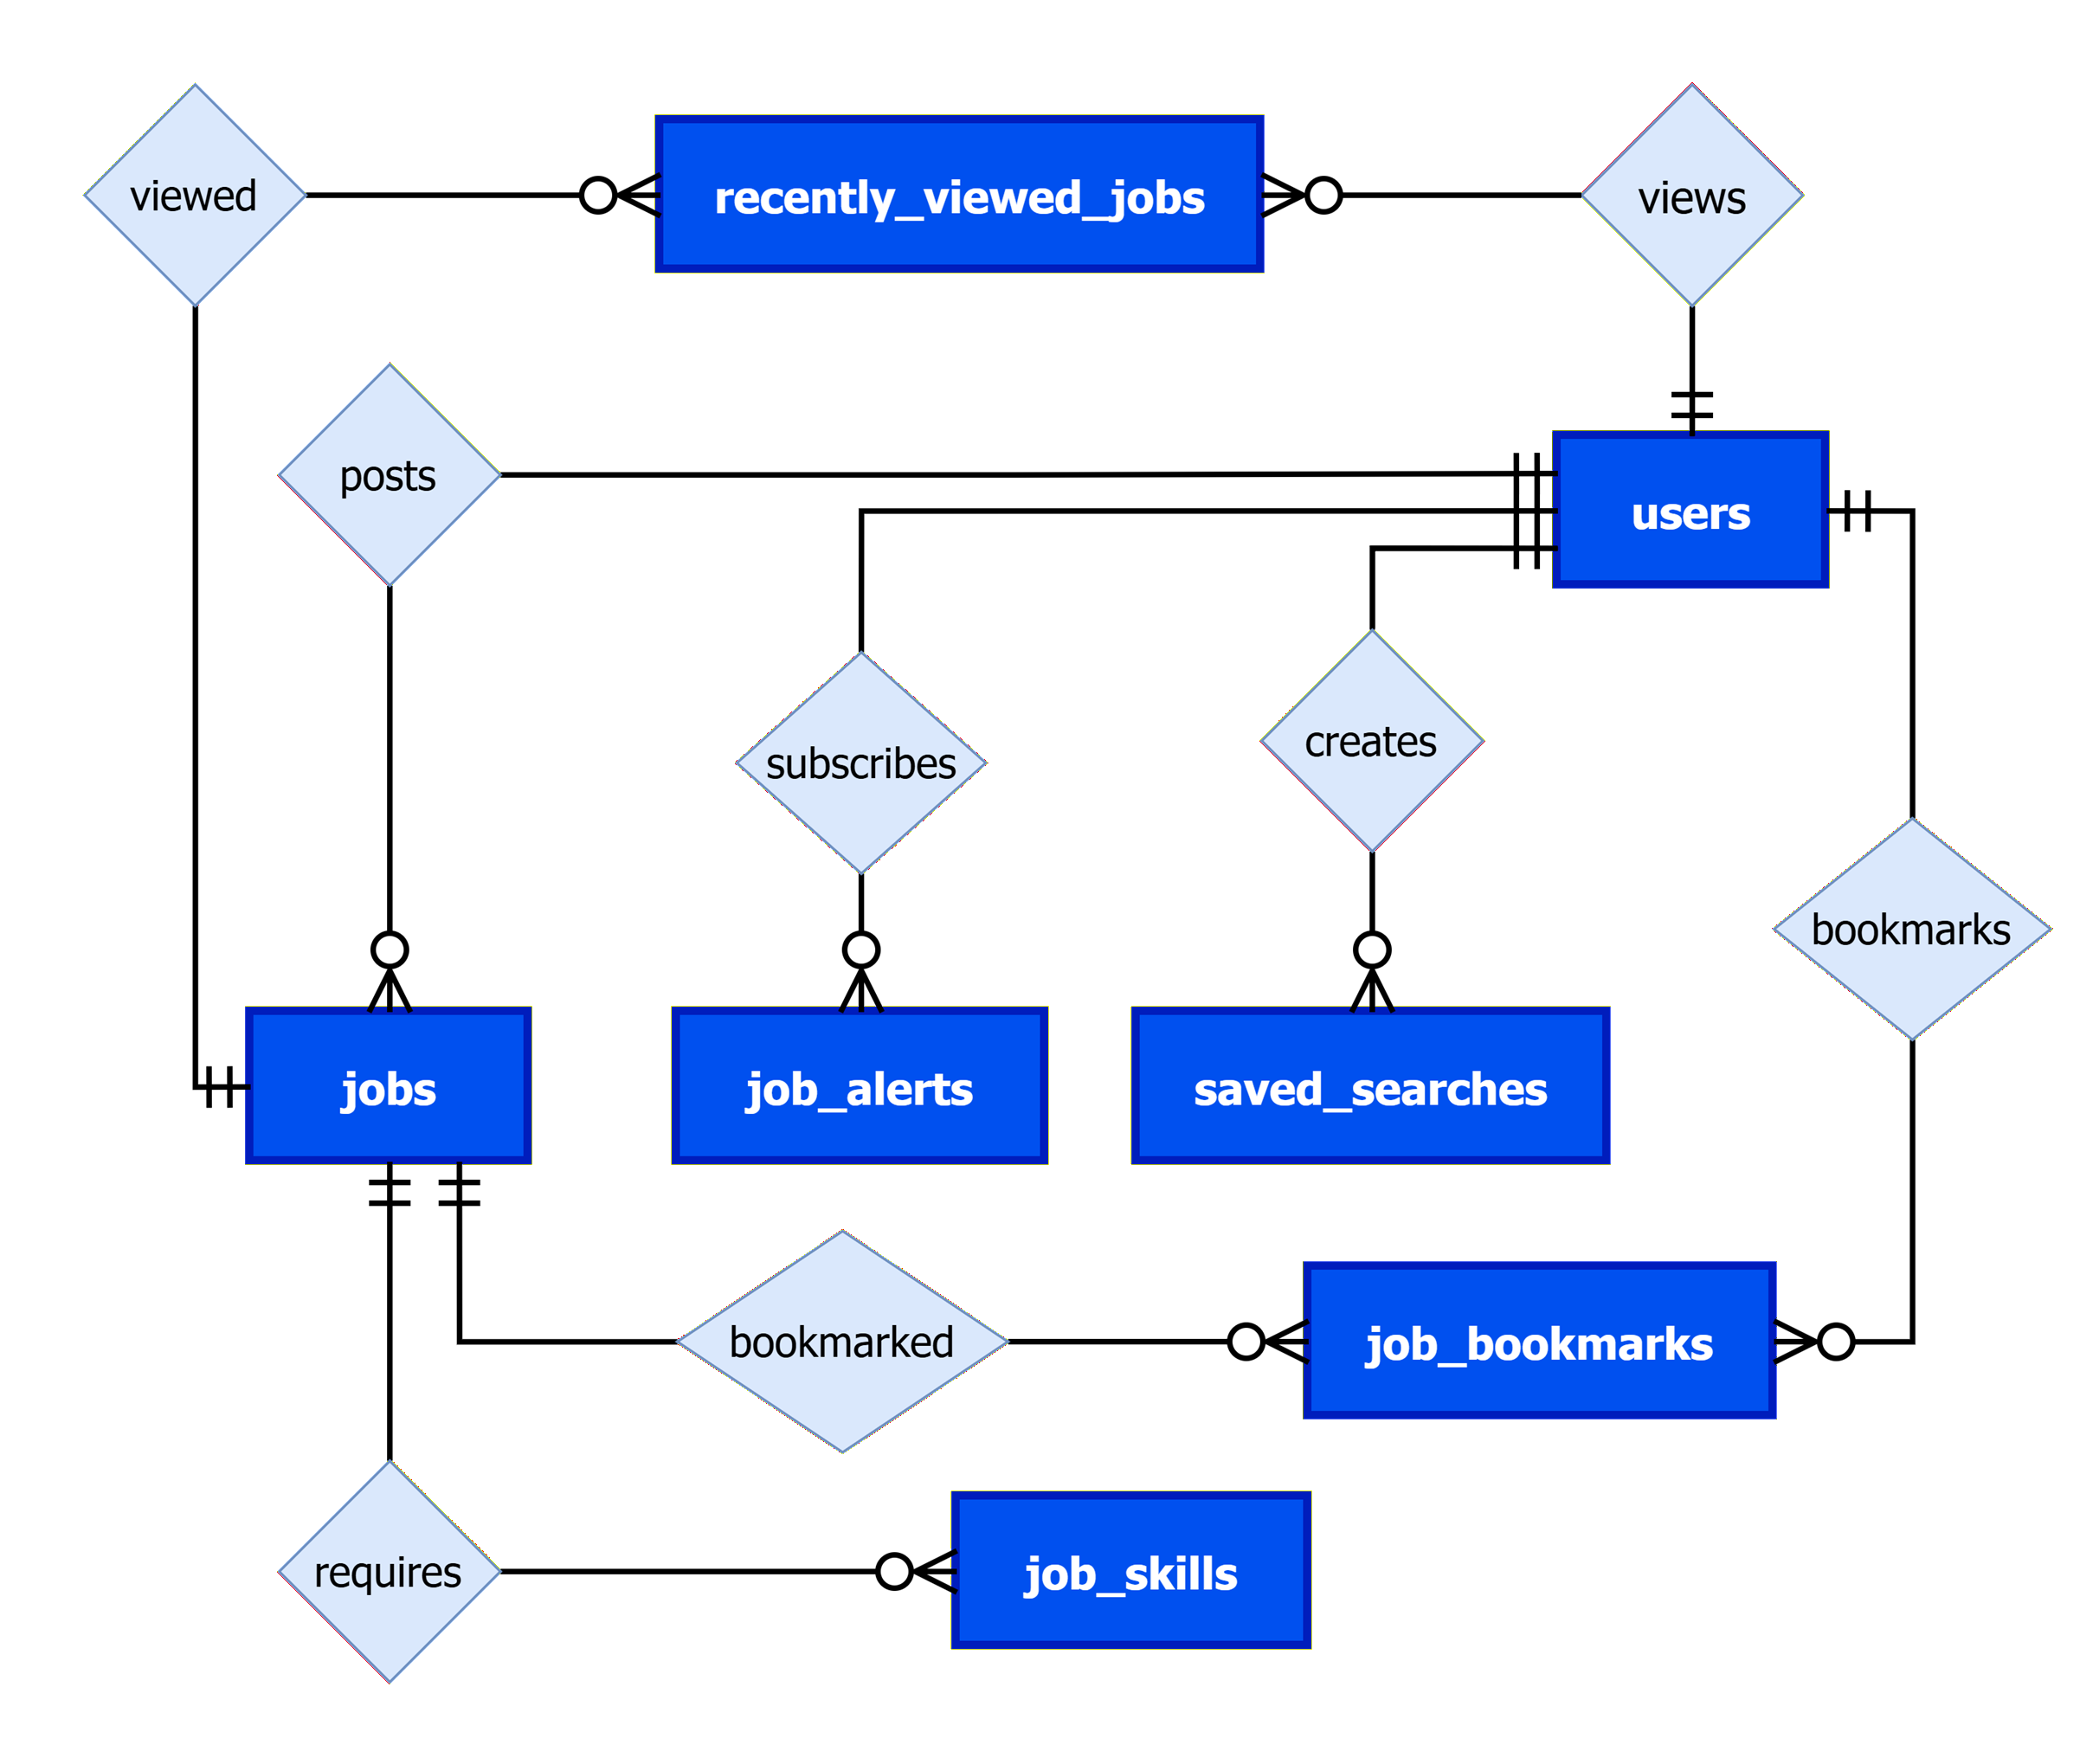
\includegraphics[width=0.95\textwidth]{image/ERD/ERD4.png}
    \caption{Job Posting \& Discovery ERD}
    \label{fig:job-posting-discovery}
\end{figure}

% ===============================================
% ERD5
% ===============================================
\paragraph{Manage Proposal}
\begin{figure}[H]
    \centering
    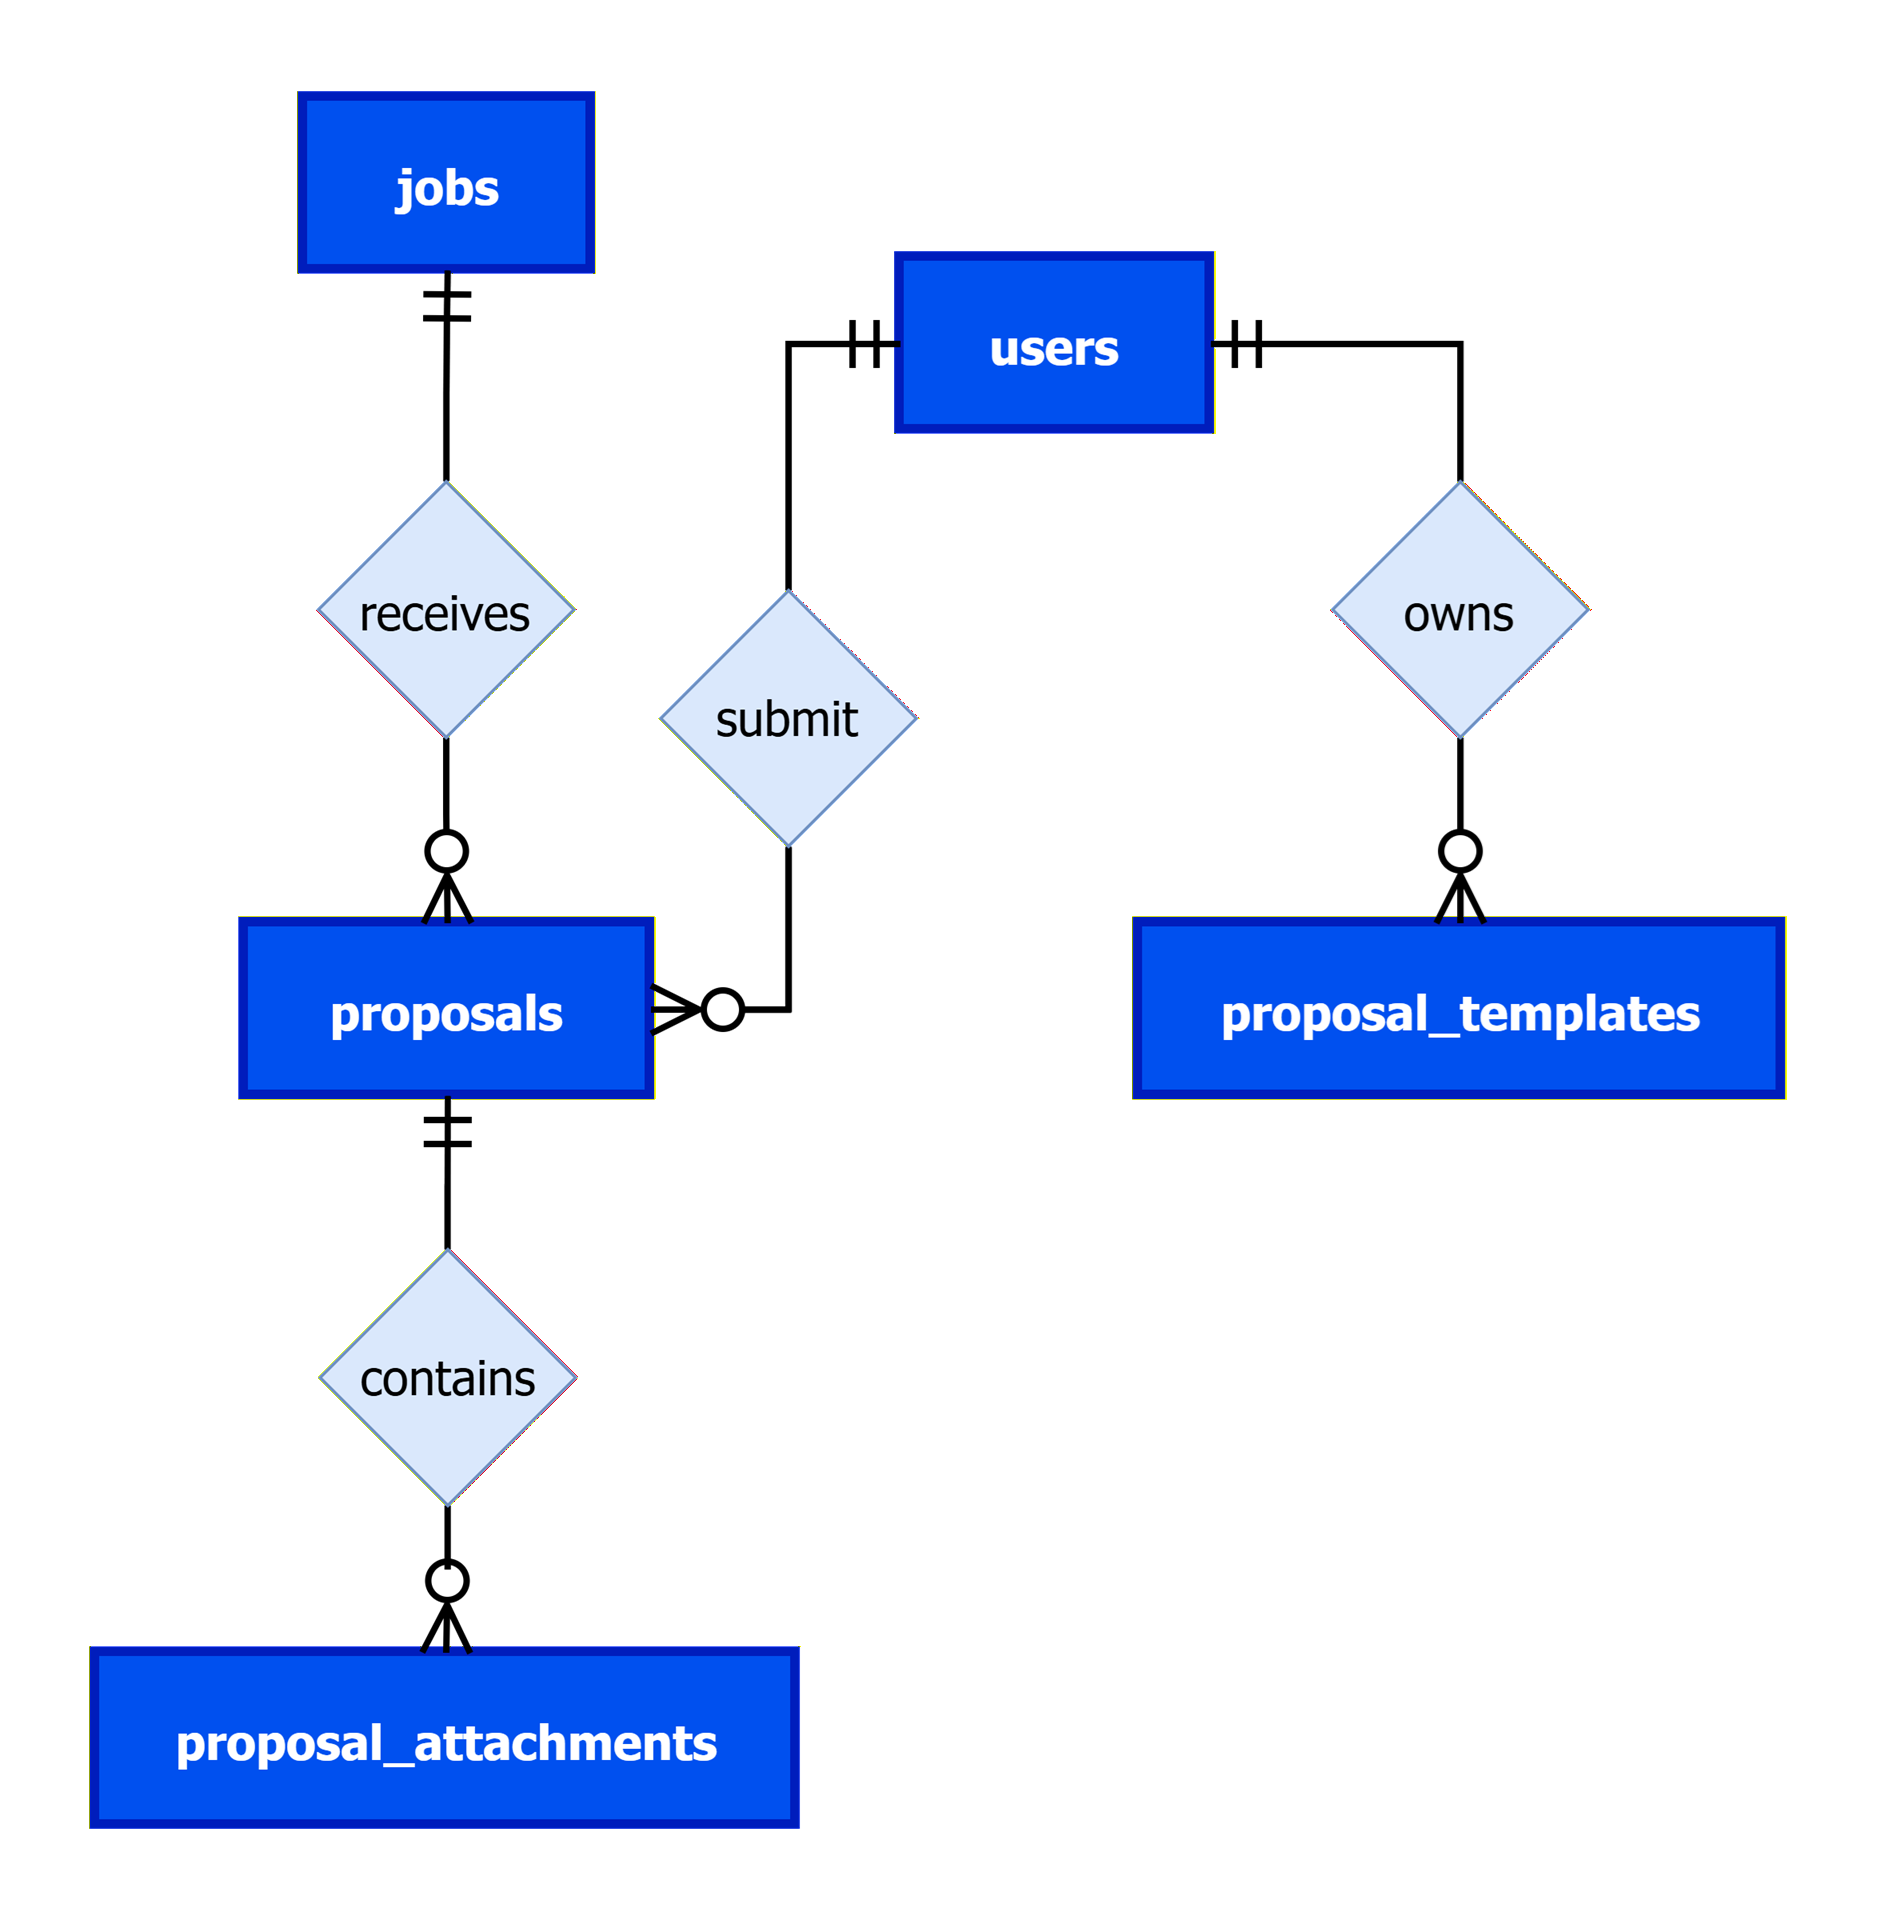
\includegraphics[width=0.95\textwidth]{image/ERD/ERD5.png}
    \caption{Manage Proposal ERD}
    \label{fig:manage-proposal}
\end{figure}

% ===============================================
% ERD6
% ===============================================
\paragraph{Manage Contract}
\begin{figure}[H]
    \centering
    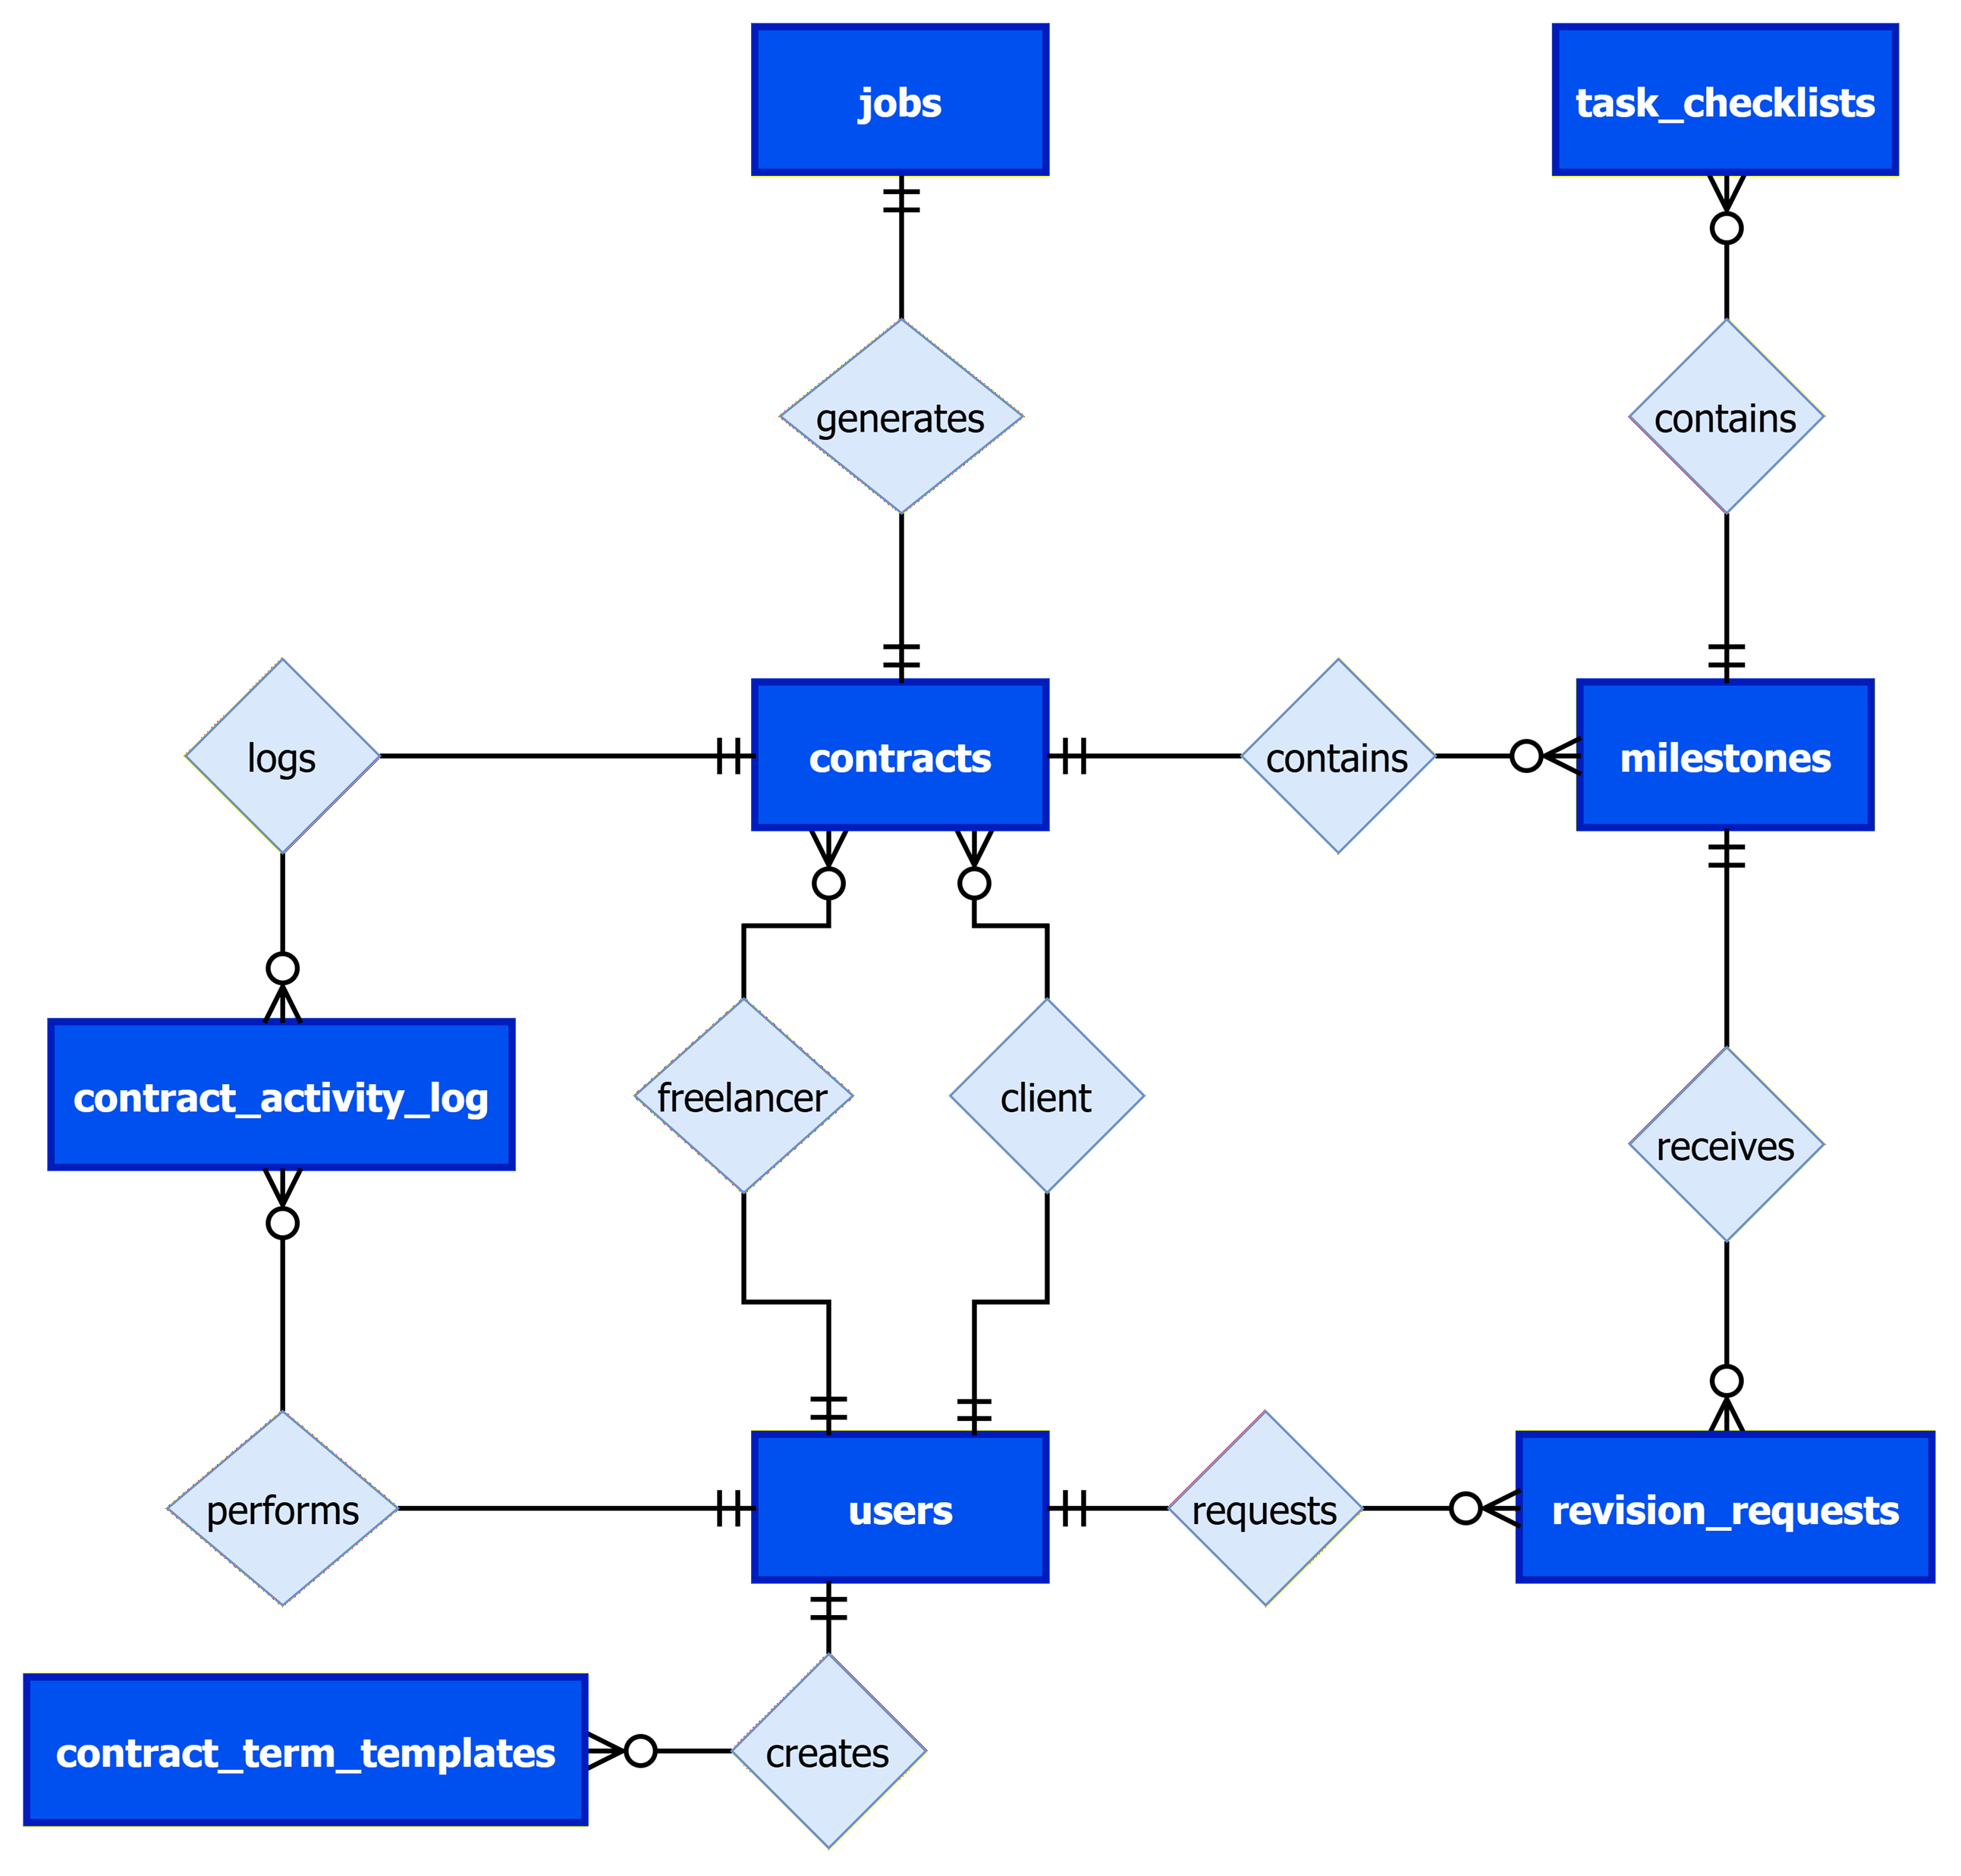
\includegraphics[width=0.95\textwidth]{image/ERD/ERD6.png}
    \caption{Manage Contract ERD}
    \label{fig:manage-contract}
\end{figure}

% ===============================================
% ERD7
% ===============================================
\paragraph{Escrow, Payments \& Dispute Resolution}
\begin{figure}[H]
    \centering
    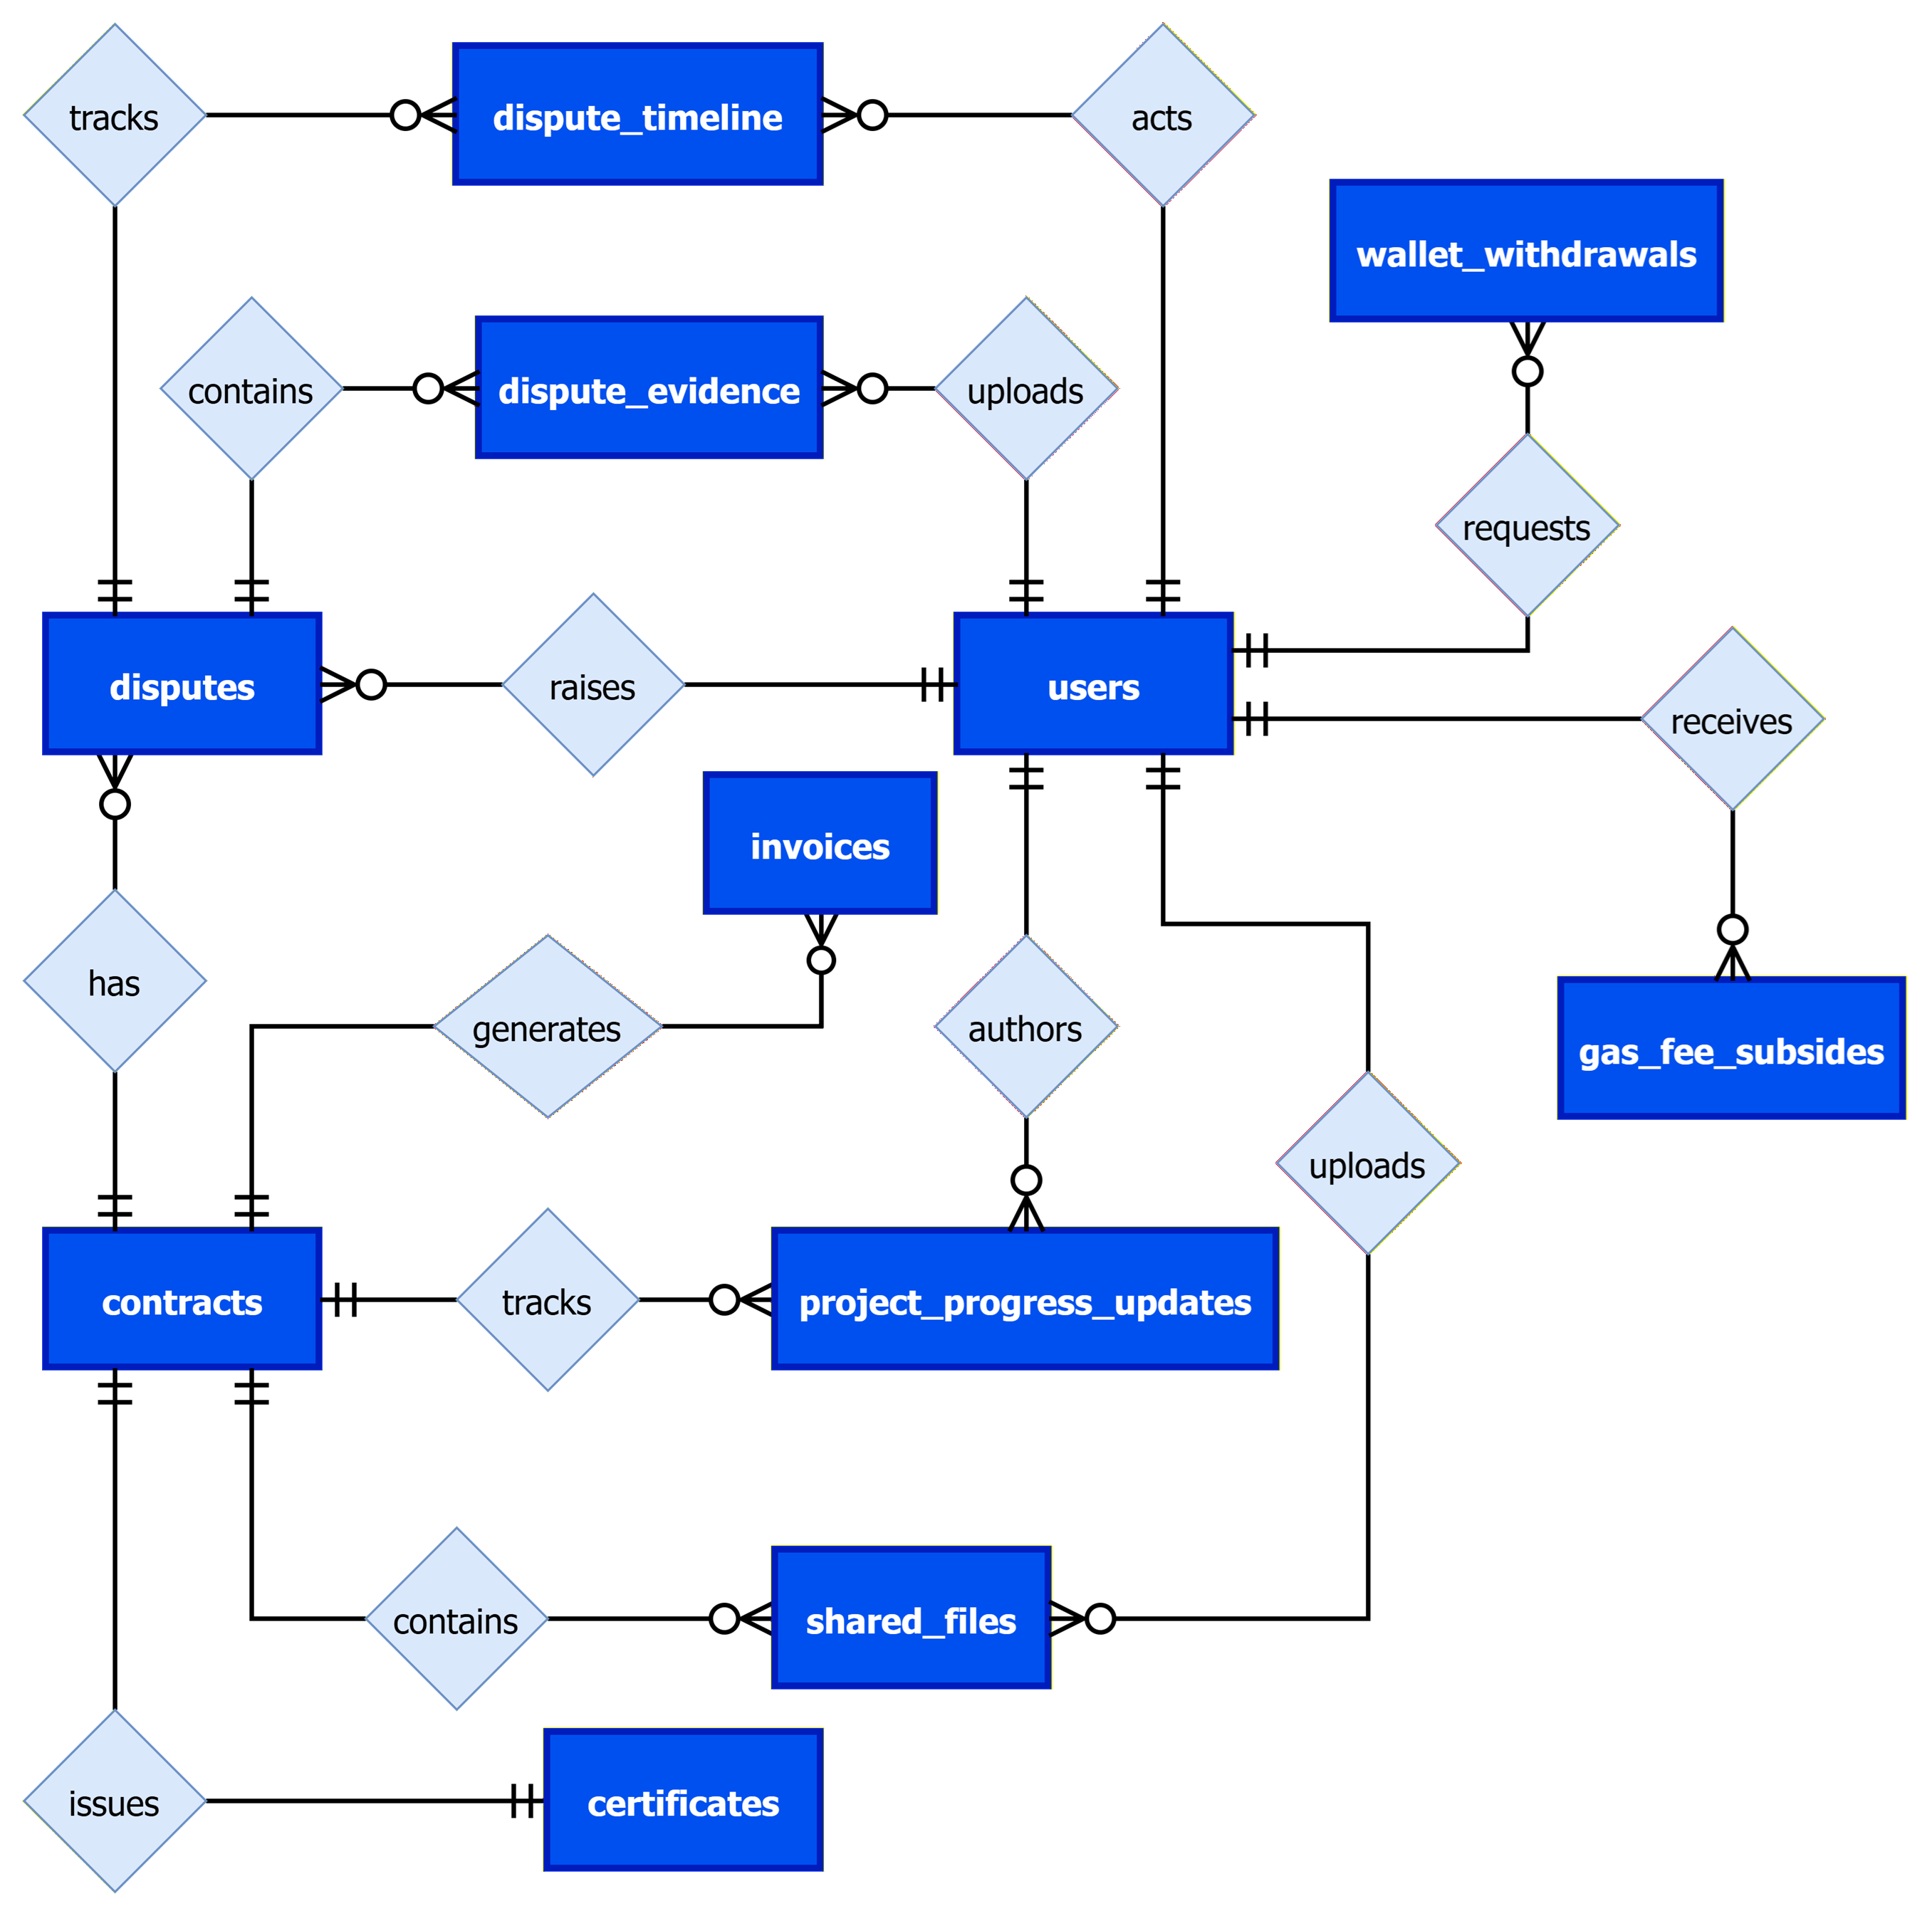
\includegraphics[width=0.95\textwidth]{image/ERD/ERD7.png}
    \caption{Escrow, Payments \& Dispute Resolution ERD}
    \label{fig:escrow-payments-dispute-resolutiont}
\end{figure}

% ===============================================
% ERD8
% ===============================================
\paragraph{Reviews \& Reputation System}
\begin{figure}[H]
    \centering
    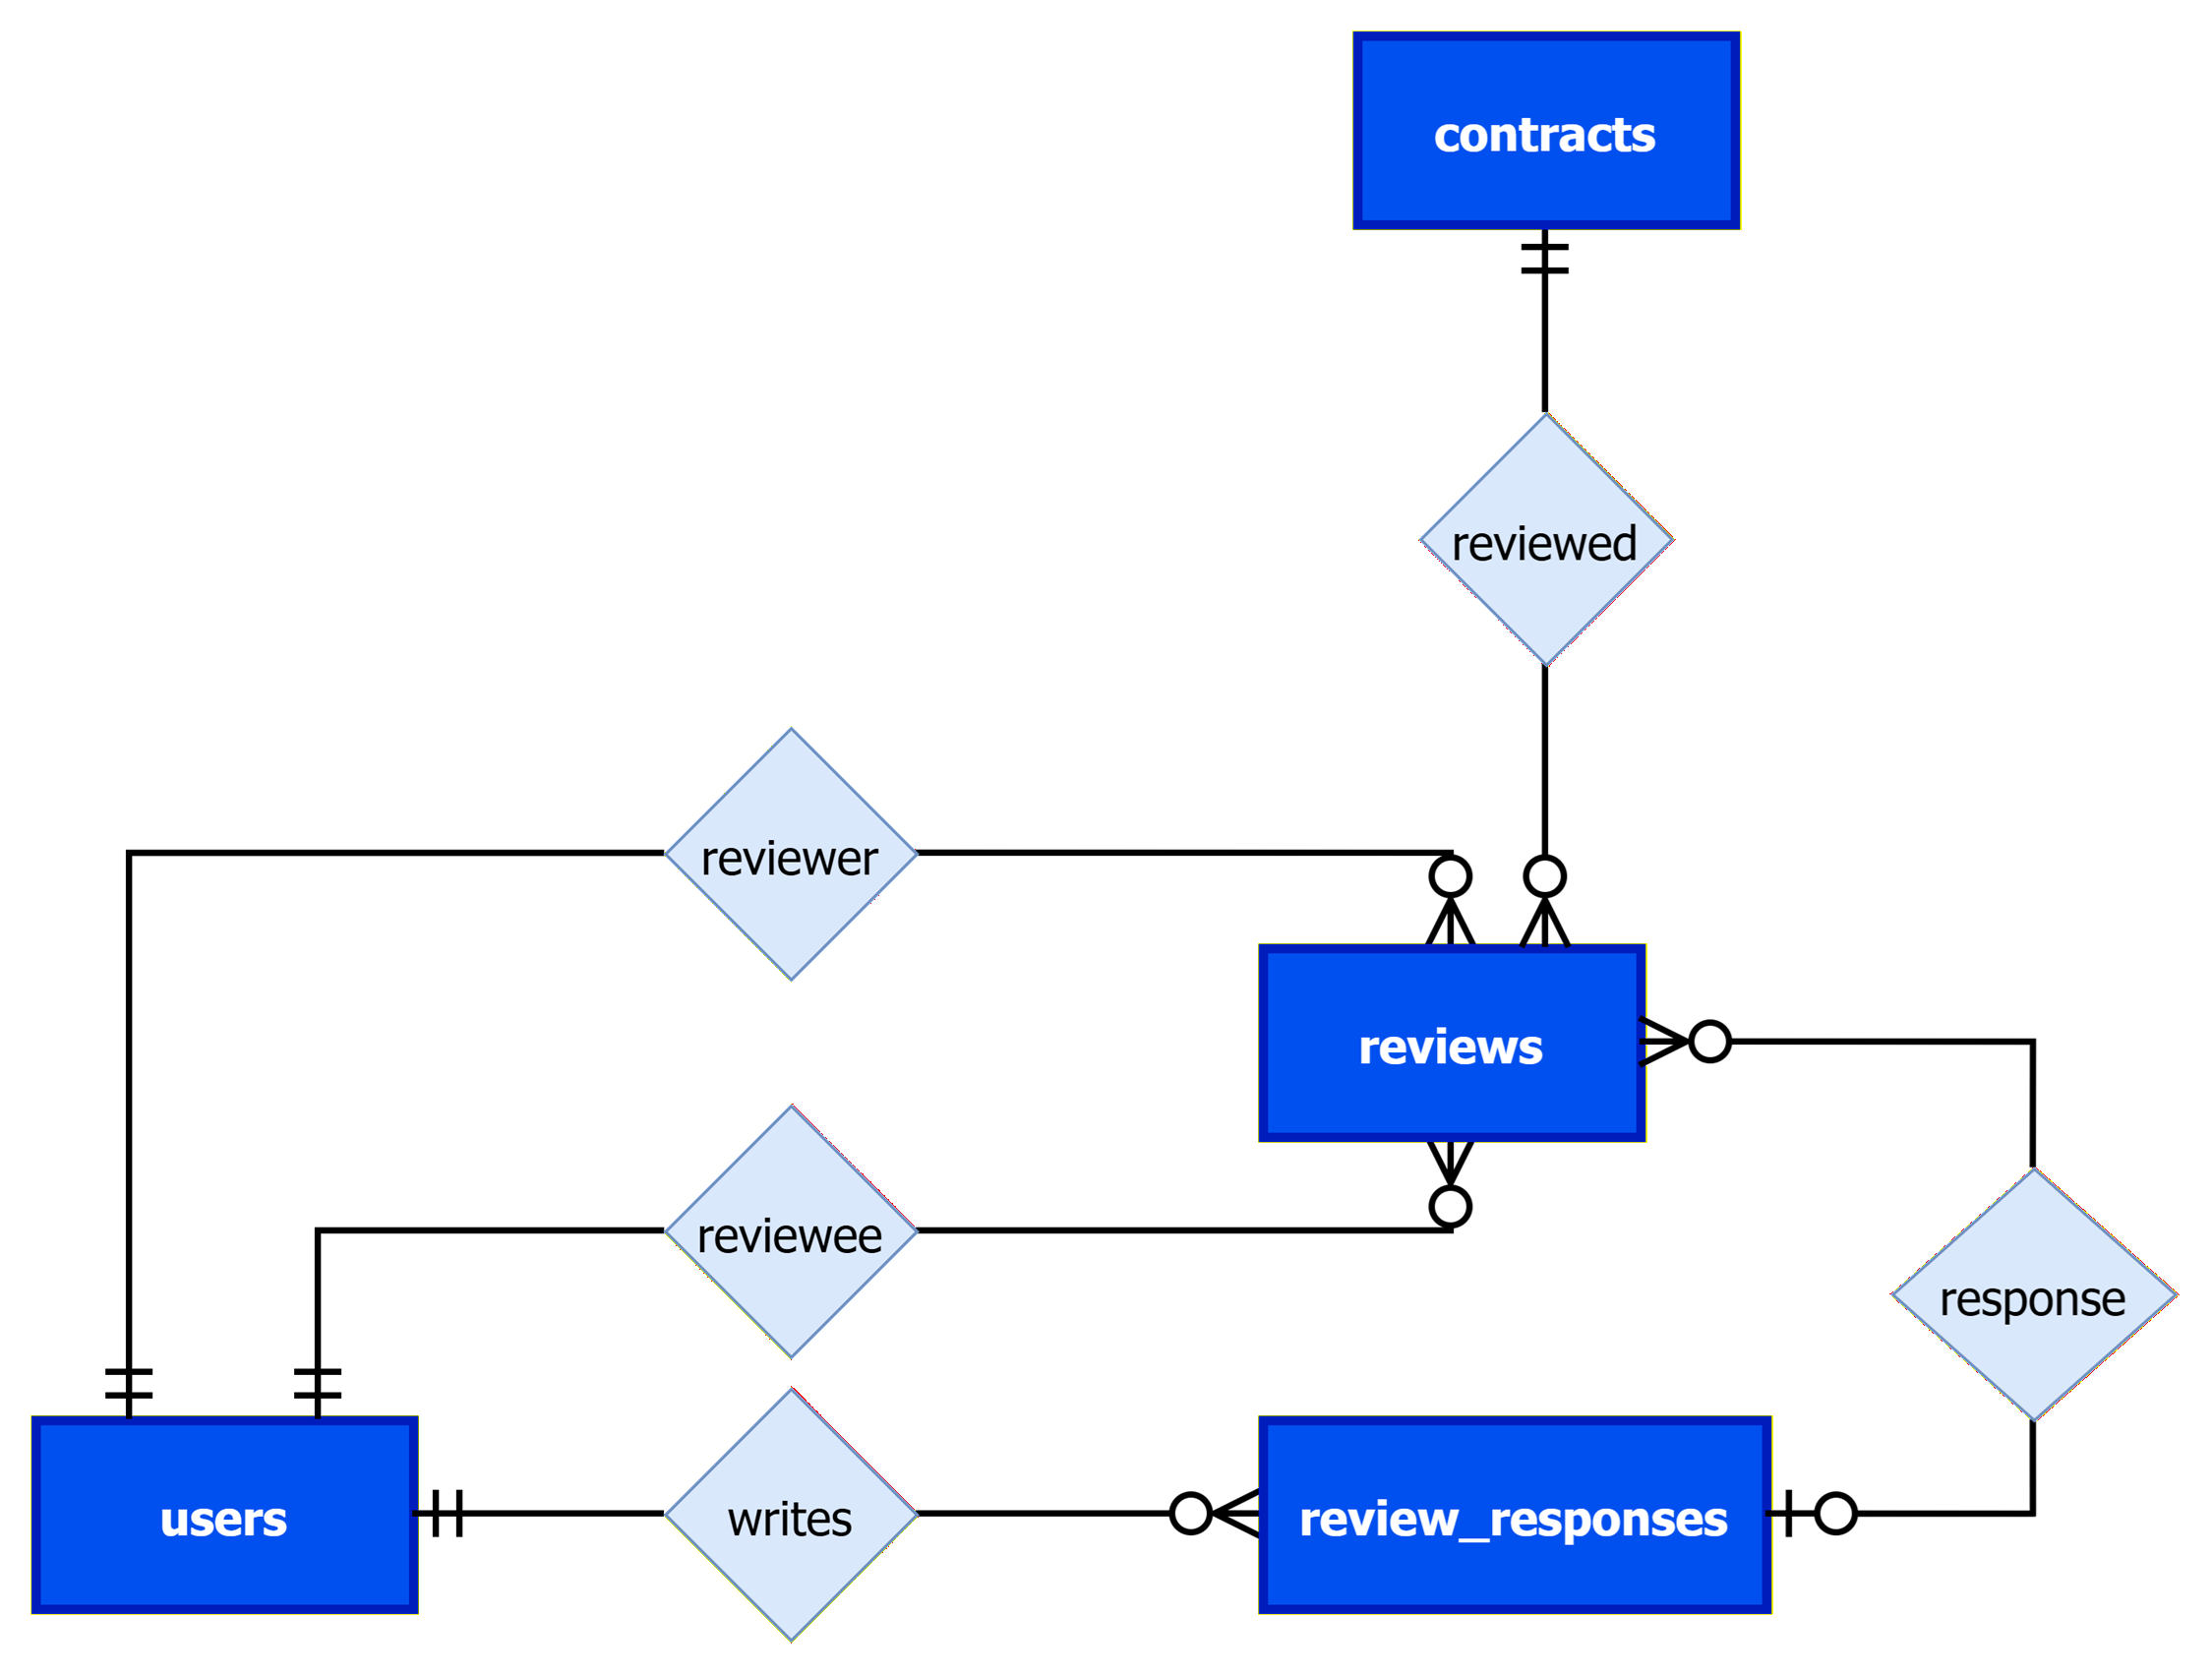
\includegraphics[width=0.95\textwidth]{image/ERD/ERD8.png}
    \caption{Reviews \& Reputation SystemERD}
    \label{fig:reviews-reputation-ystem}
\end{figure}

% ===============================================
% ERD9
% ===============================================
\paragraph{Forum \& Community}
\begin{figure}[H]
    \centering
    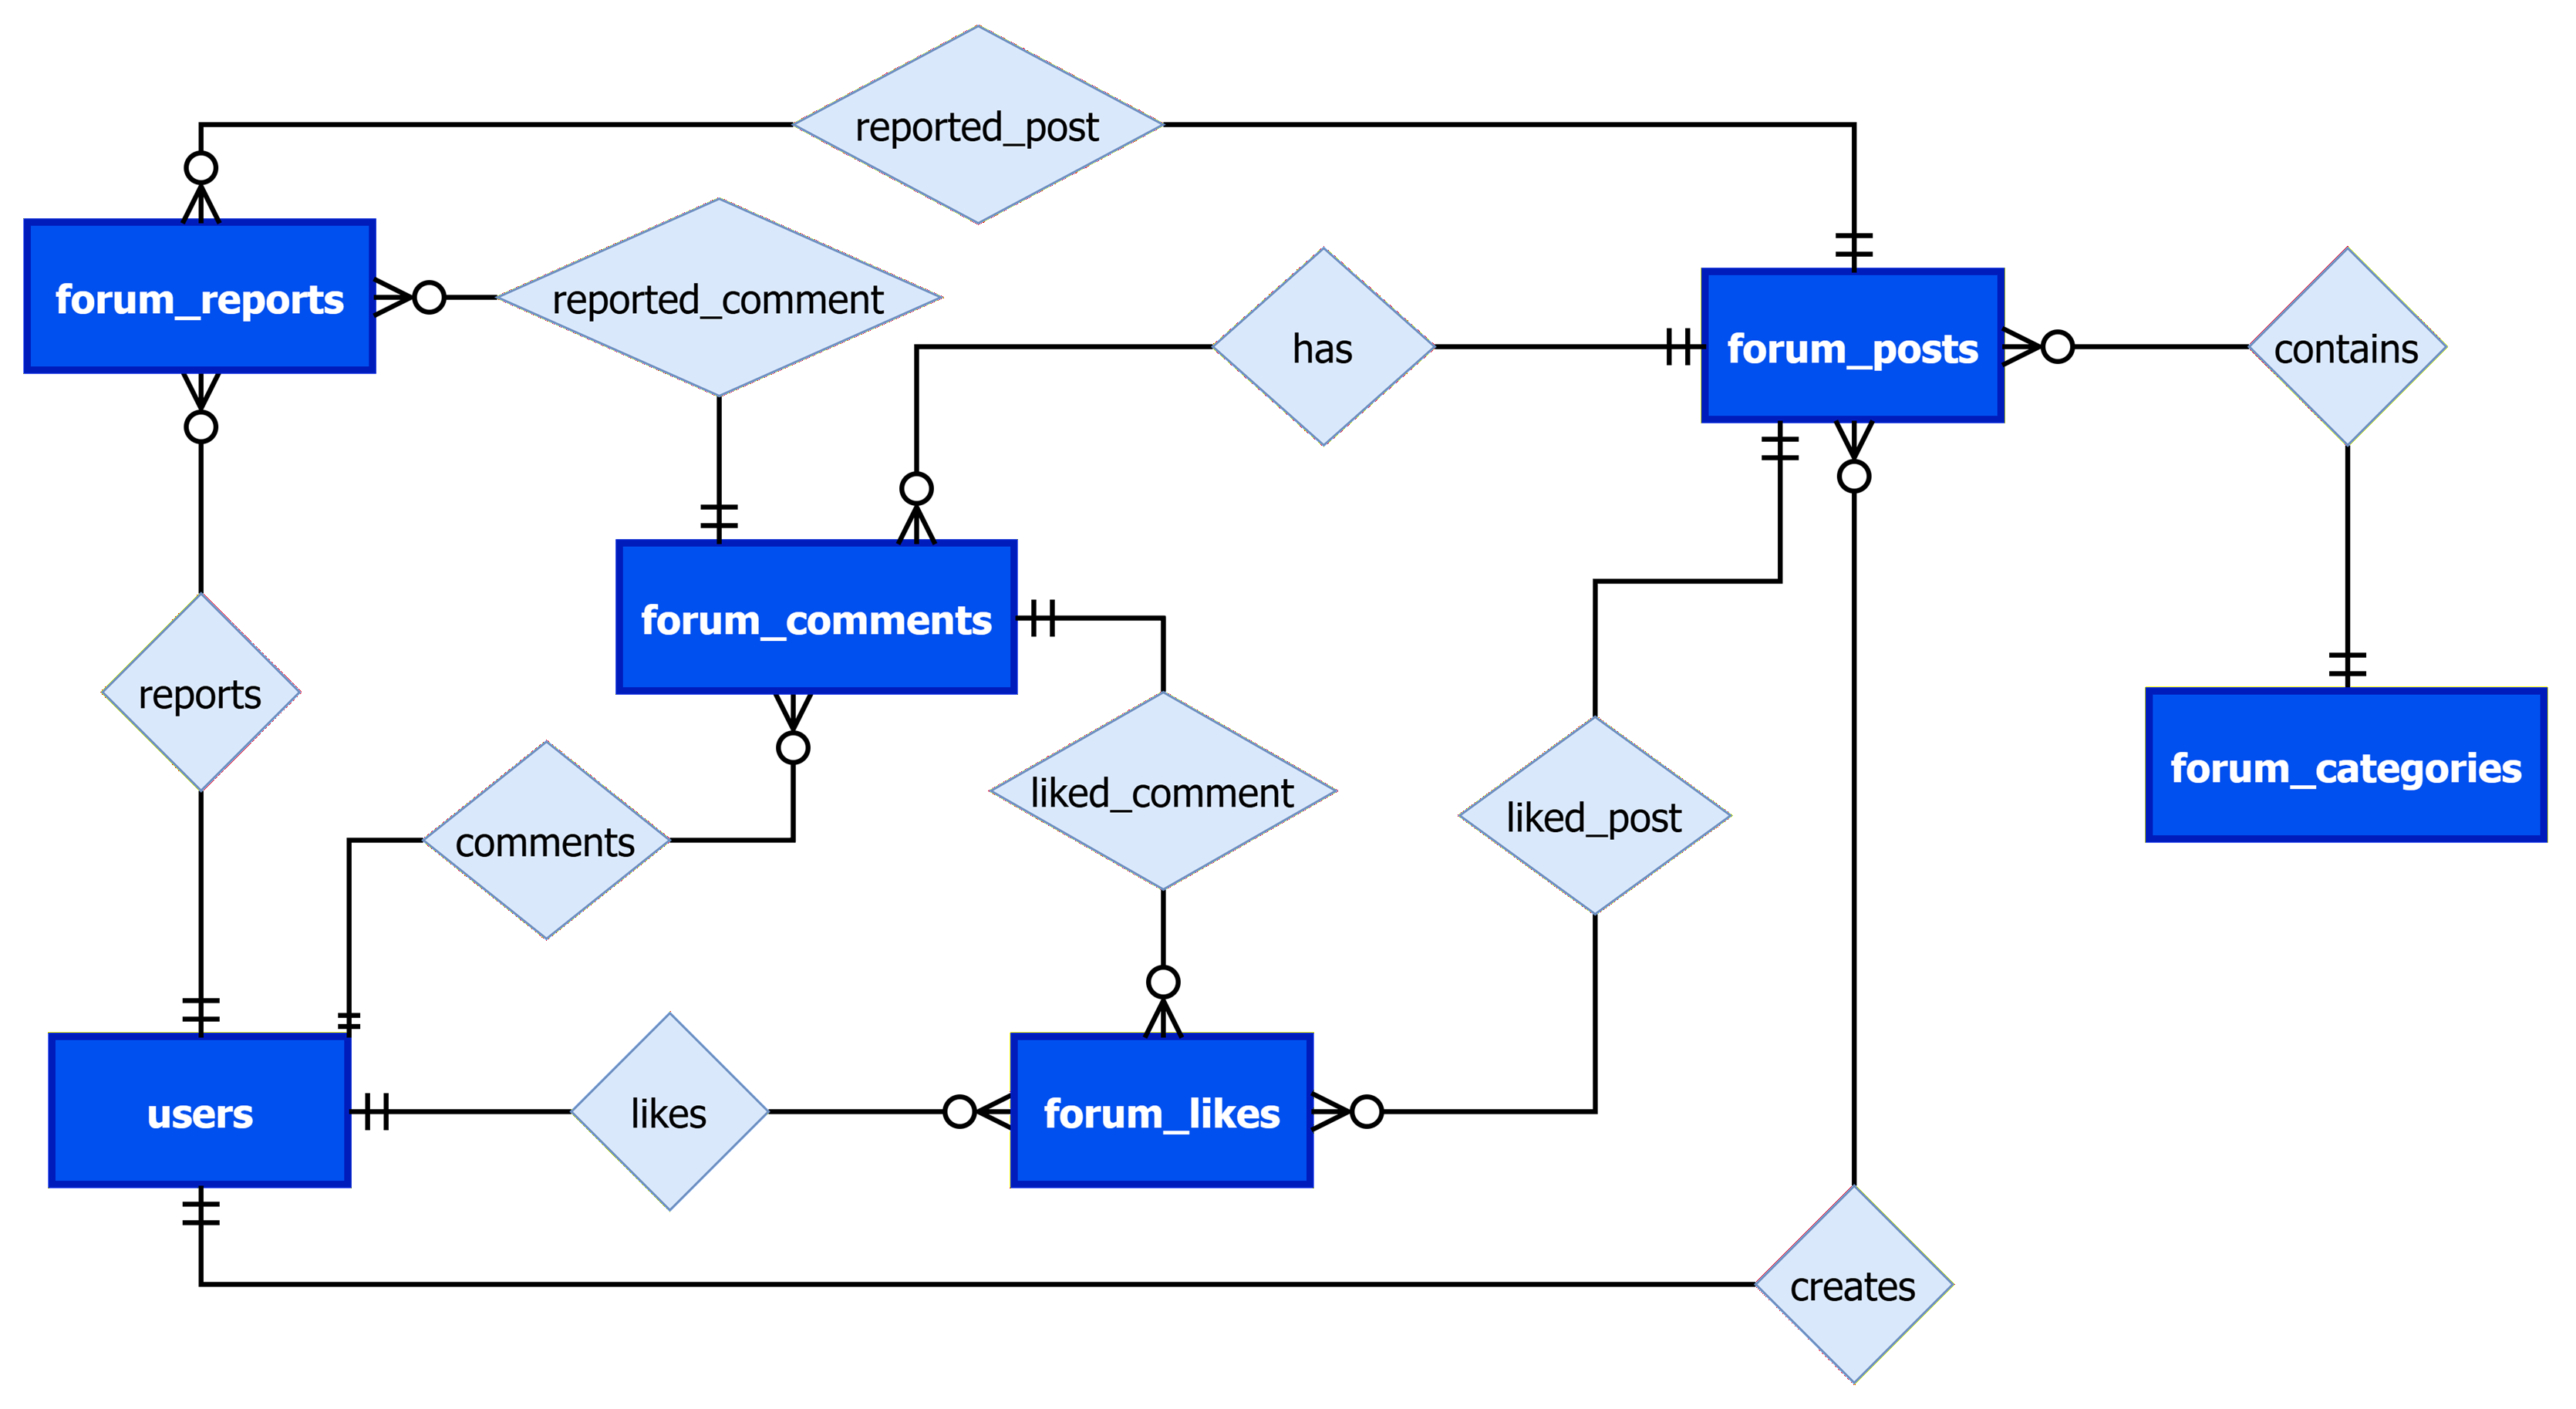
\includegraphics[width=0.95\textwidth]{image/ERD/ERD9.png}
    \caption{Forum \& Community ERD}
    \label{fig:forum-community}
\end{figure}

% ===============================================
% ERD10
% ===============================================
\paragraph{Messaging \& Notifications}
\begin{figure}[H]
    \centering
    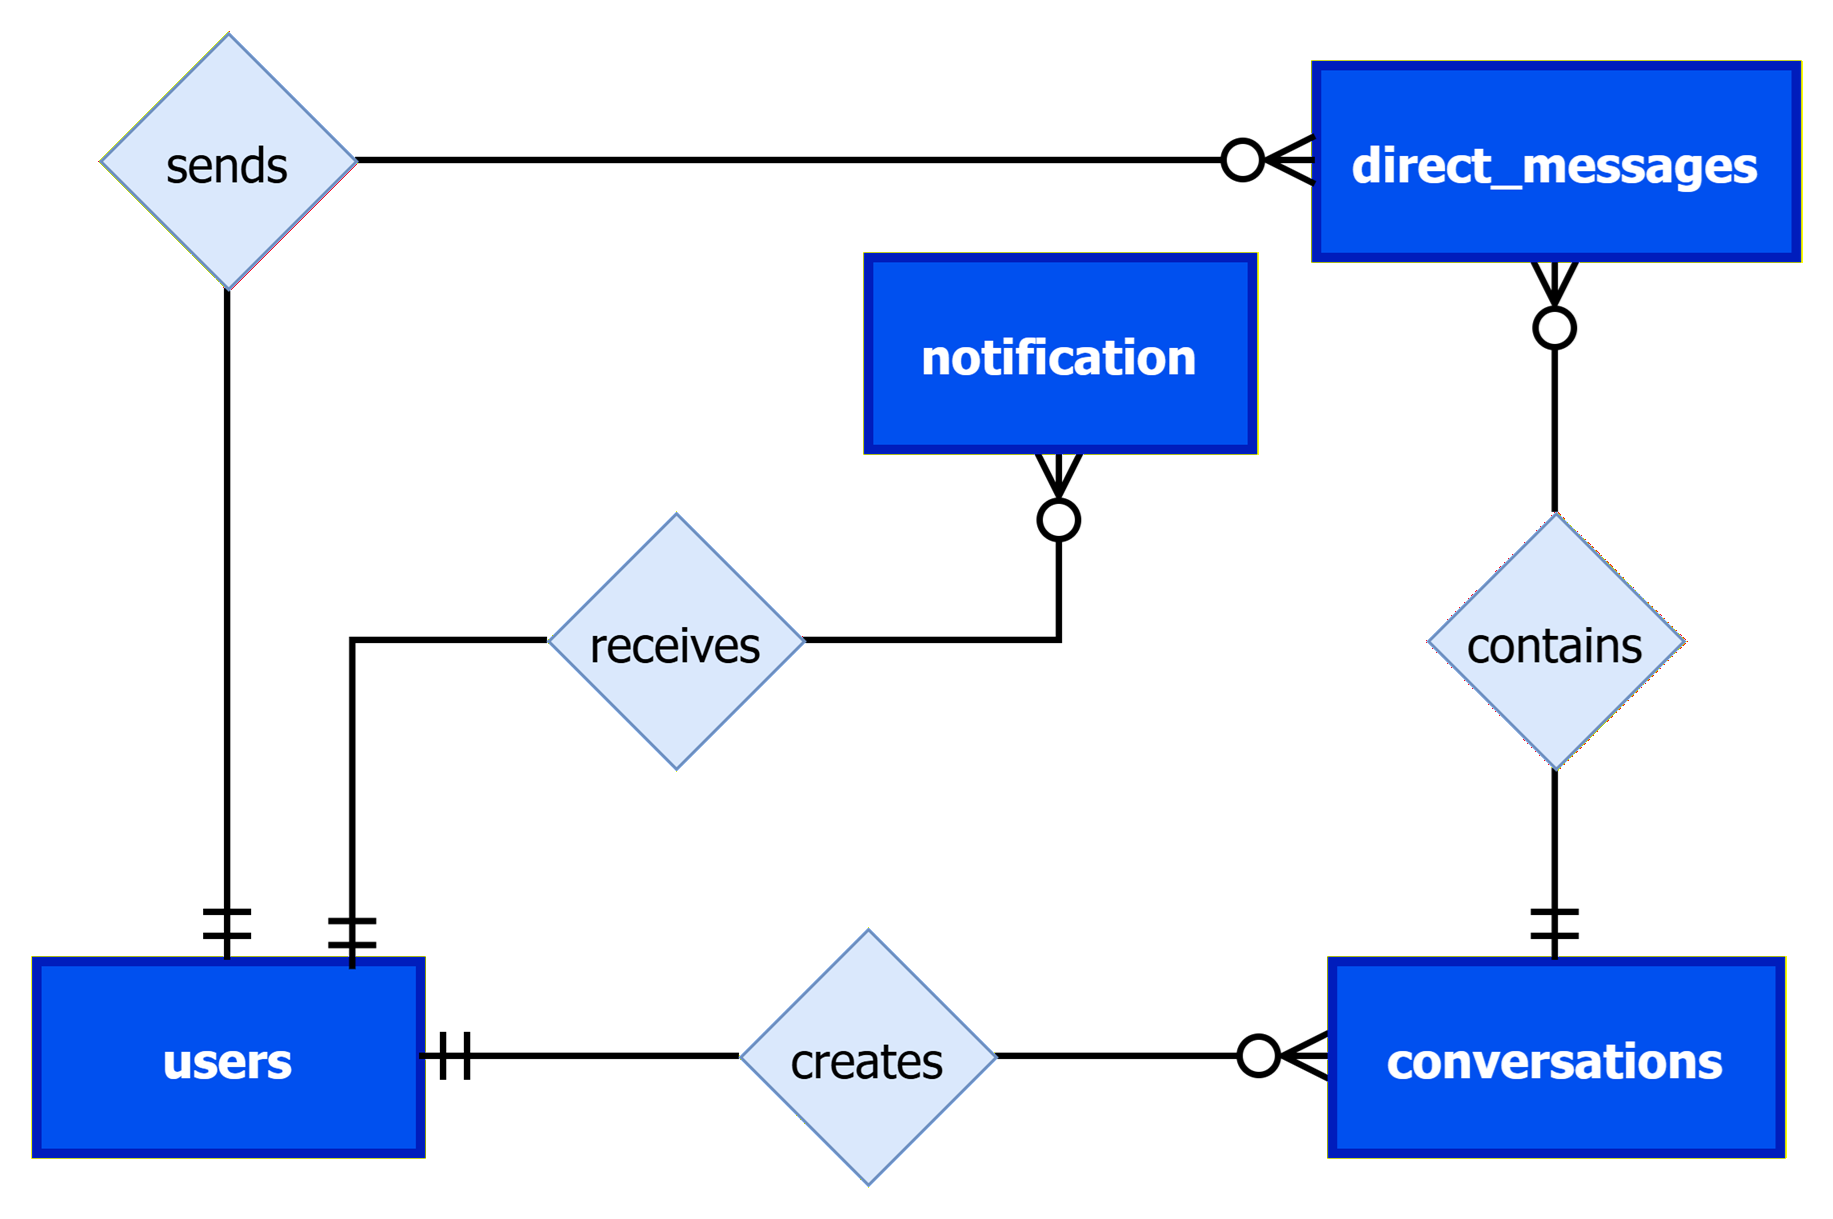
\includegraphics[width=0.95\textwidth]{image/ERD/ERD10.png}
    \caption{Messaging \& Notifications ERD}
    \label{fig:mesaging-}
\end{figure}

% ===============================================
% ERD11
% ===============================================
\paragraph{Administration \& Moderation}
\begin{figure}[H]
    \centering
    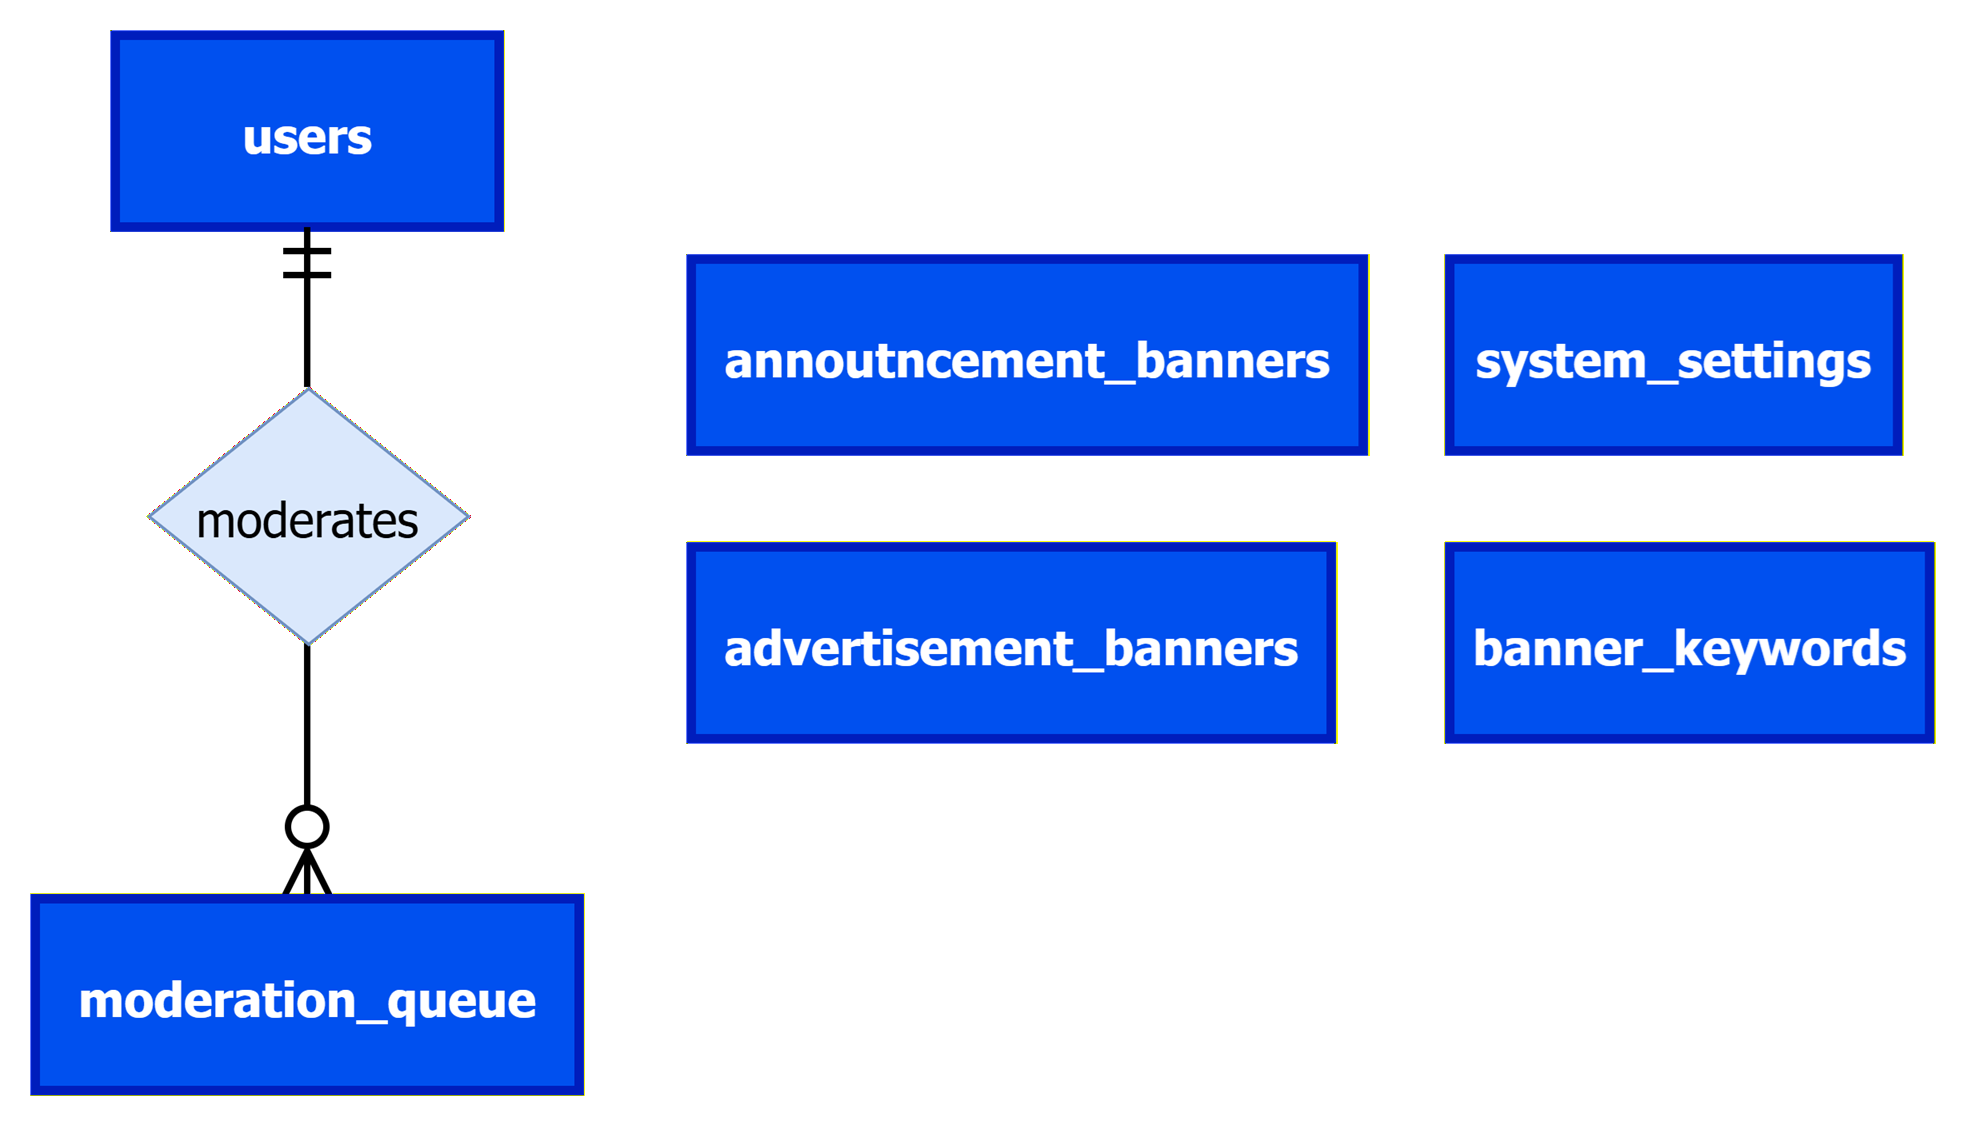
\includegraphics[width=0.95\textwidth]{image/ERD/ERD11.png}
    \caption{Administration \& Moderation ERD}
    \label{fig:administration-moderration}
\end{figure}

% ===================
% Sprint1
% ===================

% \subsection{Authentication}
% \input{sections/4.Subsections/sprint1/4.2.Authentication}

% \subsection{Manage Role}
% \input{sections/4.Subsections/sprint1/4.3.Role_Management}

% \subsection{Manage Freelancer Profile}
% \input{sections/4.Subsections/sprint1/4.4.Profile_Management}

% \subsection{Manage Freelancer Skills}
% \paragraph{Manage Freelancer Skills}
% =================================================================
% UC-05.3 Get List Freelancer Skill
% =================================================================
\subparagraph{UC-05.3 Get List Freelancer Skill}

\begin{longtable}{|L{3.2cm}|L{4.1cm}|L{2.7cm}|L{4.1cm}|}
\hline
UC ID and Name & \multicolumn{3}{l|}{UC-05.3 Get List Freelancer Skill} \\ \hline

Created By: & HuyNLN & Date Created: & DD/MM/YYYY \\ \hline

Primary Actor: & Client, Freelancer, Guest & Secondary Actors: & N/A \\ \hline

Trigger: & \multicolumn{3}{L{11.1cm}|}{When a user views a freelancer's profile or when the freelancer accesses their skills section.} \\ \hline

Description: & \multicolumn{3}{L{11.1cm}|}{Allows users to retrieve and view the complete list of skills added by a specific freelancer, including their proficiency levels.} \\ \hline

Preconditions: & \multicolumn{3}{L{11.1cm}|}{
\textbf{PRE-1} The system is connected to the database. \newline
\textbf{PRE-2} The freelancer profile exists.
} \\ \hline

Post-conditions: & \multicolumn{3}{L{11.1cm}|}{
\textbf{POST-1} The list of skills and corresponding proficiency levels associated with the freelancer is displayed.
} \\ \hline

Normal Flow: & \multicolumn{3}{L{11.1cm}|}{
\textbf{1.0 Get List Freelancer Skill} \newline
1. User accesses the freelancer's profile or skills section. \newline
2. The system queries the database to retrieve all skills associated with the freelancer's ID. \newline
3. The system loads the skill names and their respective proficiency levels. \newline
4. The system displays the list of skills to the user.
} \\ \hline

Alternative Flows: & \multicolumn{3}{L{11.1cm}|}{N/A} \\ \hline

Exceptions: & \multicolumn{3}{L{11.1cm}|}{
\textbf{1.2a No Skills Found} \newline
If the freelancer has not added any skills yet (detected at Step 2), the system displays the message: ``No skills added yet.'' \newline
Return Step 1. \newline

\textbf{1.2b Database Connection Failure} \newline
If the system cannot retrieve the skills list (detected at Step 2), it displays the message: ``Unable to load skills. Please try again later.'' \newline
Return Step 1.
} \\ \hline

Priority: & \multicolumn{3{L{11.1cm}|}{Medium} \\ \hline

Frequency of Use: & \multicolumn{3}{L{11.1cm}|}{High} \\ \hline

Business Rules: & \multicolumn{3}{L{11.1cm}|}{
BR-SKILL-01: All skills belonging to the freelancer must be displayed along with their proficiency level.
} \\ \hline

Other Information: & \multicolumn{3}{L{11.1cm}|}{N/A} \\ \hline

Assumptions: & \multicolumn{3}{L{11.1cm}|}{Skills are properly linked to the freelancer's ID in the database.} \\ \hline

\end{longtable}

% =================================================================
% UC-05.4 Add Freelancer Skill
% =================================================================

\subparagraph{UC-05.4 Add Freelancer Skill}

\begin{longtable}{|L{3.2cm}|L{4.1cm}|L{2.7cm}|L{4.1cm}|}
\hline

UC ID and Name & \multicolumn{3}{l|}{UC-05.4 Add Freelancer Skill} \\ \hline

Created By: & HuyNLN & Date Created: & DD/MM/YYYY \\ \hline

Primary Actor: & Freelancer & Secondary Actors: & N/A \\ \hline

Trigger: & \multicolumn{3}{L{11.1cm}|}{When the freelancer clicks the ``Add Skill'' button in their skills management section.} \\ \hline

Description: & \multicolumn{3}{L{11.1cm}|}{Allows an authenticated freelancer to add a new skill to their profile along with an indicating proficiency level.} \\ \hline

Preconditions: & \multicolumn{3}{L{11.1cm}|}{
\textbf{PRE-1} The freelancer is authenticated and logged in. \newline
\textbf{PRE-2} The freelancer is on their profile/skills management page.
} \\ \hline

Post-conditions: & \multicolumn{3}{L{11.1cm}|}{
\textbf{POST-1} A new skill record is created and associated with the freelancer. \newline
\textbf{POST-2} The newly added skill is displayed in the freelancer's skill list.
} \\ \hline

Normal Flow: & \multicolumn{3}{L{11.1cm}|}{
\textbf{1.0 Add Freelancer Skill} \newline
1. Freelancer clicks the ``Add Skill'' button. \newline
2. The system displays a form to input the skill. \newline
3. Freelancer enters/selects a skill name and selects a proficiency level. \newline
4. Freelancer clicks the ``Save'' button. \newline
5. The system validates the selected skill and proficiency level. \newline
6. The system checks if the skill already exists in the freelancer's profile. \newline
7. The system inserts the new skill record into the database. \newline
8. The system updates the displayed list of skills and shows a success message.
} \\ \hline

Alternative Flows: & \multicolumn{3}{L{11.1cm}|}{
\textbf{1.4 Cancel Addition} \newline
1. Freelancer clicks the ``Cancel'' button. \newline
2. The system discards the input. \newline
3. The system closes the form without making any changes.
} \\ \hline

Exceptions: & \multicolumn{3}{L{11.1cm}|}{
\textbf{1.3a Missing Required Information} \newline
If the skill name or proficiency level is not provided (entered at Step 3), the system displays the message: ``Please select a skill and a proficiency level.'' \newline
Return Step 3. \newline

\textbf{1.3b Skill Already Exists} \newline
If the freelancer tries to add a duplicate skill (entered at Step 3), the system displays: ``This skill has already been added to your profile.'' \newline
Return Step 3. \newline

\textbf{1.7 Database Connection Failure} \newline
If the system cannot save the new skill (occurs at Step 7), it displays: ``Unable to add skill. Please try again later.'' \newline
Return Step 4.
} \\ \hline

Priority: & \multicolumn{3}{L{11.1cm}|}{High} \\ \hline

Frequency of Use: & \multicolumn{3}{L{11.1cm}|}{Medium} \\ \hline

Business Rules: & \multicolumn{3}{L{11.1cm}|}{
BR-SKILL-02: A freelancer cannot add duplicate skills. \newline
BR-SKILL-03: Both skill name and proficiency level are required.
} \\ \hline

Other Information: & \multicolumn{3}{L{11.1cm}|}{Proficiency levels are typically predefined (e.g., Beginner, Intermediate, Expert).} \\ \hline

Assumptions: & \multicolumn{3}{L{11.1cm}|}{The system provides a standardized list of skills.} \\ \hline

\end{longtable}

% =================================================================
% UC-05.5 Delete Freelancer Skill
% =================================================================

\subparagraph{UC-05.5 Delete Freelancer Skill}

\begin{longtable}{|L{3.2cm}|L{4.1cm}|L{2.7cm}|L{4.1cm}|}
\hline

UC ID and Name & \multicolumn{3}{l|}{UC-05.5 Delete Freelancer Skill} \\ \hline

Created By: & HuyNLN & Date Created: & DD/MM/YYYY \\ \hline

Primary Actor: & Freelancer & Secondary Actors: & N/A \\ \hline

Trigger: & \multicolumn{3}{L{11.1cm}|}{When the freelancer clicks the ``Delete'' option next to a specific skill on their profile.} \\ \hline

Description: & \multicolumn{3}{L{11.1cm}|}{Allows a freelancer to permanently remove (hard delete) a skill from their profile.} \\ \hline

Preconditions: & \multicolumn{3}{L{11.1cm}|}{
\textbf{PRE-1} The freelancer is authenticated and logged in. \newline
\textbf{PRE-2} The skill to be deleted currently exists in the freelancer's profile.
} \\ \hline

Post-conditions: & \multicolumn{3}{L{11.1cm}|}{
\textbf{POST-1} The specific skill record is permanently deleted from the database. \newline
\textbf{POST-2} The skill is removed from the freelancer's displayed skill list.
} \\ \hline

Normal Flow: & \multicolumn{3}{L{11.1cm}|}{
\textbf{1.0 Delete Freelancer Skill} \newline
1. Freelancer clicks the ``Delete'' option for a specific skill. \newline
2. The system prompts a confirmation dialog. \newline
3. Freelancer confirms the deletion. \newline
4. The system executes a hard delete operation on the database. \newline
5. The system refreshes the skill list. \newline
6. The system displays a success message: ``Skill removed successfully.''
} \\ \hline

Alternative Flows: & \multicolumn{3}{L{11.1cm}|}{
\textbf{1.3 Cancel Deletion} \newline
1. Freelancer clicks the ``Cancel'' button in the confirmation dialog. \newline
2. The system closes the dialog. \newline
3. The skill remains on the profile.
} \\ \hline

Exceptions: & \multicolumn{3}{L{11.1cm}|}{
\textbf{1.1a Skill Not Found} \newline
If the skill record does not exist or has already been removed (triggered at Step 1), the system displays the message: ``Skill not found or already deleted.'' \newline
Return Step 1. \newline

\textbf{1.4 Database Connection Failure} \newline
If the system cannot delete the skill (occurs at Step 4), it displays the message: ``Unable to remove skill. Please try again later.'' \newline
Return Step 3.
} \\ \hline

Priority: & \multicolumn{3}{L{11.1cm}|}{Medium} \\ \hline

Frequency of Use: & \multicolumn{3}{L{11.1cm}|}{Low} \\ \hline

Business Rules: & \multicolumn{3}{L{11.1cm}|}{
BR-SKILL-04: Skill deletion must be a hard delete operation. \newline
BR-SKILL-05: Only the owning freelancer can delete a skill from their profile.
} \\ \hline

Other Information: & \multicolumn{3}{L{11.1cm}|}{N/A} \\ \hline

Assumptions: & \multicolumn{3}{L{11.1cm}|}{Deleting a skill from a freelancer's profile does not delete the core skill definition from the system's global master list.} \\ \hline

\end{longtable}

% \subsection{Manage Freelancer Portfolio}
% \input{sections/4.Subsections/sprint1/4.6.Portfolio_Management}

% \subsection{Browse Jobs}
% \input{sections/4.Subsections/sprint1/4.7.Job_Browsing}

% \subsection{Manage Job}
% % =================================================================
% UC-06.1 View List Job
% =================================================================

\subparagraph*{4.8.1 UC-06.1 View List Job}

\begin{longtable}{|L{3.2cm}|L{4.1cm}|L{2.7cm}|L{4.1cm}|}
\hline
UC ID and Name & \multicolumn{3}{l|}{UC-06.1 View List Job} \\ \hline

Created By: & Nguyen Lu Nhat Huy & Date Created: & 20/06/2026 \\ \hline

Primary Actor: & Client & Secondary Actors: & N/A \\ \hline

Trigger: & \multicolumn{3}{L{11.1cm}|}{When a client accesses the My Jobs section from the navigation menu.} \\ \hline

Description: & \multicolumn{3}{L{11.1cm}|}{As a client, I want to view a list of all jobs I have posted so that I can manage their status, review proposals, and track hiring progress.} \\ \hline

Preconditions: & \multicolumn{3}{L{11.1cm}|}{\textbf{PRE-1} The system is connected to the database. \newline \textbf{PRE-2} The client is logged in and authenticated.} \\ \hline

Post-conditions: & \multicolumn{3}{L{11.1cm}|}{\textbf{POST-1} The list of the client's own posted jobs is retrieved and displayed. \newline \textbf{POST-2} The client can select a job to view its details or proposals.} \\ \hline

Normal Flow: & \multicolumn{3}{L{11.1cm}|}{\textbf{1.0 View Own Job List} \newline 1. Client navigates to the ``My Jobs'' page. \newline 2. The system retrieves all job postings associated with the client's account ID from the \texttt{jobs} table. \newline 3. The system displays each job showing: Title, date posted, status, and the number of received proposals. \newline 4. Client selects a specific job to view details.} \\ \hline

Alternative Flows: & \multicolumn{3}{L{11.1cm}|}{N/A} \\ \hline

Exceptions: & \multicolumn{3}{L{11.1cm}|}{\textbf{1.1a No Posted Jobs Found} \newline If the client has not posted any jobs, the system displays: ``You have not posted any jobs yet.'' \newline \textbf{1.1b Database Connection Failure} \newline If the system cannot fetch data, it displays: ``Unable to load job list. Please try again later.''} \\ \hline

Priority: & \multicolumn{3}{L{11.1cm}|}{High} \\ \hline

Frequency of Use: & \multicolumn{3}{L{11.1cm}|}{High} \\ \hline

Business Rules: & \multicolumn{3}{L{11.1cm}|}{BR-JOB-01: Only jobs with client\_id equal to the authenticated user's ID shall be displayed.} \\ \hline

Other Information: & \multicolumn{3}{L{11.1cm}|}{N/A} \\ \hline

Assumptions: & \multicolumn{3}{L{11.1cm}|}{N/A} \\ \hline

\end{longtable}

% =================================================================
% UC-06.2 Post New Job
% =================================================================

\subparagraph*{4.8.2 UC-06.2 Post New Job}

\begin{longtable}{|L{3.2cm}|L{4.1cm}|L{2.7cm}|L{4.1cm}|}
\hline
UC ID and Name & \multicolumn{3}{l|}{UC-06.2 Post New Job} \\ \hline

Created By: & Nguyen Lu Nhat Huy & Date Created: & 20/06/2026 \\ \hline

Primary Actor: & Client & Secondary Actors: & N/A \\ \hline

Trigger: & \multicolumn{3}{L{11.1cm}|}{When a client clicks the ``Create Job'' button on the job listing page.} \\ \hline

Description: & \multicolumn{3}{L{11.1cm}|}{As a client, I want to create and publish a new job posting so that freelancers can apply for it.} \\ \hline

Preconditions: & \multicolumn{3}{L{11.1cm}|}{\textbf{PRE-1} The client is logged in and verified. \newline \textbf{PRE-2} The system is connected to the database.} \\ \hline

Post-conditions: & \multicolumn{3}{L{11.1cm}|}{\textbf{POST-1} A new job record is inserted with ``Active'' status in the database. \newline \textbf{POST-2} The job details are displayed on the public marketplace.} \\ \hline

Normal Flow: & \multicolumn{3}{L{11.1cm}|}{\textbf{1.0 Create and Publish Job} \newline 1. Client clicks ``Create Job'' button. \newline 2. System displays the job creation form. \newline 3. Client inputs details: Title, description, budget, required skills, and deadline. \newline 4. Client clicks ``Publish''. \newline 5. System validates inputs. \newline 6. System inserts a new record into the \texttt{jobs} table with status = 'Active'. \newline 7. System redirects the client to the Job Detail page.} \\ \hline

Alternative Flows: & \multicolumn{3}{L{11.1cm}|}{\textbf{1.3 Save as Draft} \newline 1. Client selects ``Save as Draft'' instead of ``Publish''. \newline 2. System inserts a new record into the \texttt{jobs} table with status = 'Draft'. \newline 3. System returns the client to the My Jobs list page.} \\ \hline

Exceptions: & \multicolumn{3}{L{11.1cm}|}{\textbf{1.5a Invalid Budget Input} \newline If the entered budget is lower than the minimum allowed value, the system displays: ``Budget must be greater than the minimum threshold.'' \newline \textbf{1.5b Invalid Deadline Input} \newline If the entered deadline is less than 24 hours from the current time, the system displays: ``Deadline must be at least 24 hours in the future.''} \\ \hline

Priority: & \multicolumn{3}{L{11.1cm}|}{High} \\ \hline

Frequency of Use: & \multicolumn{3}{L{11.1cm}|}{Medium} \\ \hline

Business Rules: & \multicolumn{3}{L{11.1cm}|}{BR-JOB-02: Only verified Client accounts can publish jobs. \newline BR-JOB-03: Budget must meet the system minimum threshold. \newline BR-JOB-04: Deadline must be at least 24 hours from creation.} \\ \hline

Other Information: & \multicolumn{3}{L{11.1cm}|}{N/A} \\ \hline

Assumptions: & \multicolumn{3}{L{11.1cm}|}{N/A} \\ \hline

\end{longtable}

% =================================================================
% UC-06.3 Edit Job
% =================================================================

\subparagraph*{4.8.3 UC-06.3 Edit Job}

\begin{longtable}{|L{3.2cm}|L{4.1cm}|L{2.7cm}|L{4.1cm}|}
\hline
UC ID and Name & \multicolumn{3}{l|}{UC-06.3 Edit Job} \\ \hline

Created By: & Nguyen Lu Nhat Huy & Date Created: & 20/06/2026 \\ \hline

Primary Actor: & Client & Secondary Actors: & N/A \\ \hline

Trigger: & \multicolumn{3}{L{11.1cm}|}{When a client clicks the ``Edit'' button on their job detail page.} \\ \hline

Description: & \multicolumn{3}{L{11.1cm}|}{As a client, I want to edit the details of an existing active job posting to update requirements or budget.} \\ \hline

Preconditions: & \multicolumn{3}{L{11.1cm}|}{\textbf{PRE-1} The job belongs to the logged-in client. \newline \textbf{PRE-2} The job is in ``Active'' or ``Draft'' status. \newline \textbf{PRE-3} No proposals have been accepted for this job.} \\ \hline

Post-conditions: & \multicolumn{3}{L{11.1cm}|}{\textbf{POST-1} The job record is updated in the database. \newline \textbf{POST-2} The updated details are displayed to users.} \\ \hline

Normal Flow: & \multicolumn{3}{L{11.1cm}|}{\textbf{1.0 Edit Job Details} \newline 1. Client selects a job and clicks ``Edit''. \newline 2. System displays the form pre-populated with current details. \newline 3. Client modifies the fields and clicks ``Save''. \newline 4. System validates inputs. \newline 5. System updates the record in the \texttt{jobs} table. \newline 6. System redirects the client to the updated Job Detail page.} \\ \hline

Alternative Flows: & \multicolumn{3}{L{11.1cm}|}{N/A} \\ \hline

Exceptions: & \multicolumn{3}{L{11.1cm}|}{\textbf{1.4a Edit Restricted} \newline If the job status is already ``In Progress'' or ``Closed'', the system displays: ``This job cannot be edited because a contract has been signed.''} \\ \hline

Priority: & \multicolumn{3}{L{11.1cm}|}{Medium} \\ \hline

Frequency of Use: & \multicolumn{3}{L{11.1cm}|}{Low} \\ \hline

Business Rules: & \multicolumn{3}{L{11.1cm}|}{BR-JOB-05: Editing is restricted if there are accepted proposals or signed contracts.} \\ \hline

Other Information: & \multicolumn{3}{L{11.1cm}|}{N/A} \\ \hline

Assumptions: & \multicolumn{3}{L{11.1cm}|}{N/A} \\ \hline

\end{longtable}

% =================================================================
% UC-06.4 Delete Job
% =================================================================

\subparagraph*{4.8.4 UC-06.4 Delete Job}

\begin{longtable}{|L{3.2cm}|L{4.1cm}|L{2.7cm}|L{4.1cm}|}
\hline
UC ID and Name & \multicolumn{3}{l|}{UC-06.4 Delete Job} \\ \hline

Created By: & Nguyen Lu Nhat Huy & Date Created: & 20/06/2026 \\ \hline

Primary Actor: & Client & Secondary Actors: & N/A \\ \hline

Trigger: & \multicolumn{3}{L{11.1cm}|}{When a client clicks the ``Delete'' button on their job listing or detail page.} \\ \hline

Description: & \multicolumn{3}{L{11.1cm}|}{As a client, I want to delete a job posting so that it is removed from the public marketplace.} \\ \hline

Preconditions: & \multicolumn{3}{L{11.1cm}|}{\textbf{PRE-1} The job belongs to the logged-in client. \newline \textbf{PRE-2} The database is active.} \\ \hline

Post-conditions: & \multicolumn{3}{L{11.1cm}|}{\textbf{POST-1} The job status is updated to ``Deleted'' in the database. \newline \textbf{POST-2} The job is removed from public marketplace view.} \\ \hline

Normal Flow: & \multicolumn{3}{L{11.1cm}|}{\textbf{1.0 Delete Job Posting} \newline 1. Client clicks ``Delete'' icon/button. \newline 2. System displays a confirmation dialog. \newline 3. Client clicks ``Confirm''. \newline 4. System updates the status of the job in the \texttt{jobs} table to 'Deleted'. \newline 5. System refreshes the job list and shows a success toast.} \\ \hline

Alternative Flows: & \multicolumn{3}{L{11.1cm}|}{N/A} \\ \hline

Exceptions: & \multicolumn{3}{L{11.1cm}|}{N/A} \\ \hline

Priority: & \multicolumn{3}{L{11.1cm}|}{High} \\ \hline

Frequency of Use: & \multicolumn{3}{L{11.1cm}|}{Low} \\ \hline

Business Rules: & \multicolumn{3}{L{11.1cm}|}{BR-JOB-06: Deleted jobs remain in the database for auditing and dispute history but are hidden from the marketplace.} \\ \hline

Other Information: & \multicolumn{3}{L{11.1cm}|}{N/A} \\ \hline

Assumptions: & \multicolumn{3}{L{11.1cm}|}{N/A} \\ \hline

\end{longtable}

% =================================================================
% UC-06.5 Change Job Status
% =================================================================

\subparagraph*{4.8.5 UC-06.5 Change Job Status}

\begin{longtable}{|L{3.2cm}|L{4.1cm}|L{2.7cm}|L{4.1cm}|}
\hline
UC ID and Name & \multicolumn{3}{l|}{UC-06.5 Change Job Status} \\ \hline

Created By: & Nguyen Lu Nhat Huy & Date Created: & 20/06/2026 \\ \hline

Primary Actor: & Client & Secondary Actors: & N/A \\ \hline

Trigger: & \multicolumn{3}{L{11.1cm}|}{When a client clicks the toggle or status dropdown (e.g. Pause, Reopen, Close) on their job detail page.} \\ \hline

Description: & \multicolumn{3}{L{11.1cm}|}{As a client, I want to change the status of a job posting to control proposal submissions.} \\ \hline

Preconditions: & \multicolumn{3}{L{11.1cm}|}{\textbf{PRE-1} The job belongs to the logged-in client. \newline \textbf{PRE-2} The job is active.} \\ \hline

Post-conditions: & \multicolumn{3}{L{11.1cm}|}{\textbf{POST-1} The job status is updated in the database. \newline \textbf{POST-2} Users see the updated status on the job details screen.} \\ \hline

Normal Flow: & \multicolumn{3}{L{11.1cm}|}{\textbf{1.0 Toggle Status} \newline 1. Client selects a new status (e.g. 'Paused') from the dropdown on the Job Detail page. \newline 2. The system updates the status of the job in the \texttt{jobs} table. \newline 3. The page refreshes, and the new status is displayed.} \\ \hline

Alternative Flows: & \multicolumn{3}{L{11.1cm}|}{N/A} \\ \hline

Exceptions: & \multicolumn{3}{L{11.1cm}|}{N/A} \\ \hline

Priority: & \multicolumn{3}{L{11.1cm}|}{Medium} \\ \hline

Frequency of Use: & \multicolumn{3}{L{11.1cm}|}{Medium} \\ \hline

Business Rules: & \multicolumn{3}{L{11.1cm}|}{BR-JOB-07: Paused or Closed jobs do not accept new proposal submissions.} \\ \hline

Other Information: & \multicolumn{3}{L{11.1cm}|}{N/A} \\ \hline

Assumptions: & \multicolumn{3}{L{11.1cm}|}{N/A} \\ \hline

\end{longtable}



% \subsection{Manage Contract}
% \input{sections/4.Subsections/sprint1/4.9.Contract_Management}

% \subsection{Manage Forum}
% \input{sections/4.Subsections/sprint1/4.10.Forum_Management}

% ===================
% Sprint2
% ===================
\section{Non-Functional Requirement}
This section describes the non-functional requirements of the Frevia platform, covering performance, security, availability, usability, and Web3-specific requirements.

\subsection{Performance \& Scalability}
\begin{itemize}
    \item \textbf{Response Time:} The system's API read operations must respond within 200ms under normal load (up to 500 concurrent requests). Write/update operations, excluding blockchain transactions, must complete within 500ms.
    \item \textbf{Page Load Time:} The web application must achieve a Largest Contentful Paint (LCP) of less than 2.5 seconds, adhering to Google's Core Web Vitals guidelines.
    \item \textbf{Concurrency:} The system backend must support at least 1,000 concurrent active users and handle a database connection pool efficiently.
    \item \textbf{Search and Filtering Efficiency:} The job search page must employ debouncing (300ms delay) and pagination (default 10 items per page) to optimize query performance and reduce server load.
\end{itemize}

\subsection{Security \& Privacy}
\begin{itemize}
    \item \textbf{Authentication and Authorization:} All network communications must be encrypted using HTTPS/TLS 1.3. User passwords must be hashed using bcrypt with a work factor of 12.
    \item \textbf{Session Management:} JWT Access Tokens must have a short lifespan (e.g., 15 minutes) and be stored in memory. Refresh Tokens must have a longer lifespan (e.g., 7 days), be stored in HTTP-only, Secure, and SameSite=Strict cookies, and be invalidated in the database upon user logout.
    \item \textbf{Role-Based Access Control (RBAC):} The system must strictly enforce role boundaries (Guest, Freelancer, Client, Admin). Administrative features, such as changing smart contract addresses or viewing audit logs, must be blocked by a server-side gateway for non-admin accounts.
    \item \textbf{Web3 Wallet and Transaction Safety:} Input wallet addresses must be verified on the client and server side to conform to the standard EVM format (starts with \texttt{0x} followed by 40 hexadecimal characters).
\end{itemize}

\subsection{Availability \& Reliability}
\begin{itemize}
    \item \textbf{System Uptime:} The system core services must maintain a 99.9\% monthly uptime, excluding scheduled maintenance.
    \item \textbf{Blockchain Fault Tolerance:} In case of RPC node connection failures, the platform must gracefully fall back to backup RPC endpoints within 3 seconds to avoid breaking the wallet balance display or transaction signing flows.
    \item \textbf{Escrow Reliability:} Funds locked in the Escrow Smart Contracts must be secure. Contracts must be verified on Etherscan/BscScan and use standard libraries (e.g., OpenZeppelin) to prevent vulnerabilities.
\end{itemize}

\subsection{Usability \& User Experience}
\begin{itemize}
    \item \textbf{Responsive Design:} The user interface must be fully responsive, supporting mobile devices, tablets, and desktop viewports (minimum width 320px).
    \item \textbf{Toast Notification System:} Interactive toast notifications (success, warning, error) must have the highest z-index to overlay all content, auto-dismiss after 3000ms, and must not freeze or block other user interactions.
    \item \textbf{Client-side Image Processing:} The avatar cropping tool must handle images locally before upload. The system must restrict upload sizes to under 5MB and validate formats (.jpg, .jpeg, .png, .webp) before initiating API requests.
\end{itemize}

\end{document}